\documentclass{ou-report}

% Dit template is gemaakt door P.J. Molijn in het kader van zijn afstuderen aan de OU in 2014.
% Waarvoor hartelijk dank.
% Minieme maar belangrijke wijzigingen zijn aangebracht door E.M. van Doorn
% Het template is versimpeld door Sylvia Stuurman, 2019.
% Het template is van extra aanwijzingen voorzien door Sylvia Stuurman, 2021.


%\hypersetup{
%pdfsubject={Master Thesis <Titel>, <author>},
%pdfkeywords={keyword1, keyword2}
%}

\setlist{nosep}

\begin{document}
\newcommand{\todo}[1]{{\color{red} #1}}
\pagestyle{plain}
\title{Browser-based port scanning}
\author{ing. Bas van de Louw}
%Title of the thesis
%\title[Subtitle]{Title}
%\author{author}
%\affiliation{
%\begin{tabular}{ll}
%Student: & studentnumber \\
%Date:    & DD/MM/YYY \\
%\end{tabular}
%}
%
%%\coverimage{cover/cover.jpg}
%%            ===============
%\makecover[frontboxwidth=4.6in]
\begin{titlepage}

\begin{center}

%% Insert the OU logo at the bottom of the page.
\begin{tikzpicture}[remember picture,overlay]
    \node at (current page.south)[anchor=south,inner sep=0pt]{
        
\includegraphics[scale=0.7]{cover/logo}
    };
\end{tikzpicture}

%% Extra whitespace at the top.
\vspace*{2\bigskipamount}

%% Print the title in specific color.
{\makeatletter
%\titlestyle\color{ou-cyan}\Huge\@title
\titlestyle\color{red}\Huge\@title{}
\makeatother}

%% Print the optional subtitle in black.
{\makeatletter
\ifx\@subtitle\undefined\else
    \bigskip
    \titlefont\titleshape\LARGE\@subtitle{}
\fi
\makeatother}

\bigskip
\bigskip

by
%door

\bigskip
\bigskip

%% Print the name of the author.
{\makeatletter
\titlefont\Large\bfseries\@author{}
\makeatother}

\vfill

in partial fulfillment of the requirements for the degree of
%in overeenstemming met de vereisten voor het verkrijgen van de graad van

\bigskip
\bigskip

{\bfseries Master of Science}

in Software Engineering

\bigskip
\bigskip

at the Open University, faculty of Management, Science and Technology \\
Master Software Engineering
%aan de Open Universiteit Nederland,

to be defended publicly on Day Month DD, YYYY at HH:00 PM.\@
%in het openbaar te verdedigen op dinsdag 9 september om 15:00 uur.

\vfill

\begin{tabular}{lll}
%% Add additional information here, per faculty requirements, e.g
    Student number: & student number \\
    Course code: & IMA0002\\
    Thesis committee:
        & titles and name of the chairman (chairman), & Open University \\
        & titles and name of the supervisor (supervisor), & Open University
\end{tabular}

%% Only include the following lines if confidentiality is applicable.
\bigskip


\bigskip

\end{center}

\end{titlepage} 


%% Use Roman numerals for the page numbers of the title pages and table of
%% contents.
\pagenumbering{roman}
%% Include an optional title page.

\frontmatter 


\let\cleardoublepage\clearpage

% Optional Dedication, Acknowledgement
%\input{dedication}

%\input{acknowledgement}


%Optional: list of figures, list of tables
%\listoffigures

%\listoftables

%% Include an optional summary page.
%\chapter*{Abstract}

This paper presents a study on browser-based port scanning, a technique that allows for the detection of open ports on a target system through the use of a web browser. The research investigates the optimal strategy for browser-based port scanning, the feasibility of using port scanning to identify specific programs running on a user's system, and the uniqueness of browser-based port scanning fingerprints.

The study demonstrates that browser-based port scanning can serve as an effective alternative to traditional port scanning techniques. The results suggest that browser-based port scanning can accurately identify specific programs running on a user's system. This has concerning implications because browser-based port scanning is a client-side, local operation on the user's system, unlike regular port scanning, which might be leveraged to bypass intrusion detection systems, such as a firewall.

Furthermore, the study estimates the uniqueness of browser-based port scanning fingerprints, which has significant implications for user privacy and internet anonymity. The study reveals that browser-based port scanning fingerprints are distinct enough to be employed as a means of tracking users across various websites, highlighting the need for enhanced privacy measures by modern web browsers.  
%\input{Summary/samenvatting}


\pagenumbering{arabic}

\chapter*{Acknowledgements}

If you would like to, you can thank people here
\chapter*{Abstract}

This paper presents a study on browser-based port scanning, a technique that allows for the detection of open ports on a target system through the use of a web browser. The research investigates the optimal strategy for browser-based port scanning, the feasibility of using port scanning to identify specific programs running on a user's system, and the uniqueness of browser-based port scanning fingerprints.

The study demonstrates that browser-based port scanning can serve as an effective alternative to traditional port scanning techniques. The results suggest that browser-based port scanning can accurately identify specific programs running on a user's system. This has concerning implications because browser-based port scanning is a client-side, local operation on the user's system, unlike regular port scanning, which might be leveraged to bypass intrusion detection systems, such as a firewall.

Furthermore, the study estimates the uniqueness of browser-based port scanning fingerprints, which has significant implications for user privacy and internet anonymity. The study reveals that browser-based port scanning fingerprints are distinct enough to be employed as a means of tracking users across various websites, highlighting the need for enhanced privacy measures by modern web browsers.  

\tableofcontents

\mainmatter{}

\chapter{Introduction}
% You can start your report by copying the introduction from your VAF. The advice is to rewrite the introduction \emph{after} you did write the remainder of the thesis.

% In the introduction, you:

% \begin{itemize}
% 	\item motivate why this research is important. You can bring forward motivation with respect to society, or show that your research is scientifically interesting; preferably both
% 	\item give some background information
% 	\item describe the goal of your research
% 	\item give the reader an overview of the structure of the remainder of your thesis.
% \end{itemize}

% This sentence is only here to show you how to refer to a source~\citep{Dijkstra-1968}.

% \begin{table}[h!tbp]
% \begin{tabular}{l | r | r| c}
% kolom 1 & kolom 2 & kolom 3 & kolom 4 \\
% \hline
% zon & maan & ster & meteoor\\
% gras & graan & groen & grauw\\
% \end{tabular}
% \caption{Example table}
% \label{table-example}
% \end{table}

% Table~\ref{table-example} shows how to include a table. Note that the first column is left-justified, the right column is centered, and the other two columns are right-justified (because of the \texttt{\{l | r | r | c\}}). More information: \url{https://en.wikibooks.org/wiki/LaTeX/Tables}. 

% \texttt{[h!tb]} means: preferably place the table \emph{h}ere, and if that is not possible, at the \emph{t}op of the page, at the \emph{b}ottom, or on a separate \emph{page}. The same positioning advice can be used in figures. Figure~\ref{fig-example} is an example.

% \begin{figure}[h!tbp]
% 
\includegraphics[scale=0.5]{LaTeX.png}
% \caption{LaTeX}
% \label{fig-example}
% \end{figure}

% The following chapters are an example of how you could structure your thesis. Do not hesitate to use a different structure!

As the world becomes more digitized, online privacy and user tracking have become major concerns. Websites are collecting vast amounts of data about their visitors, including sensitive information about their devices and browsing behavior. Websites often collect user data, such as search queries, IP addresses, and click behavior, through tracking technologies like cookies and web beacons. The collection of this data can be used for various purposes, such as targeted advertising, personalization, and user profiling.
 
Several studies have explored the implications of user tracking and privacy. Acar et al.~\citescientific{acar2014} found that a significant number of websites are capable of tracking users across multiple visits, posing a potential threat to user privacy. In a similar vein, Mayer and \\ Mitchell~\citescientific{mayer2012} have examined the privacy implications of third-party tracking on the web and have proposed measures for policymakers and developers to address these concerns.

Furthermore, the privacy risks associated with personalized advertising have been analyzed by Komanduri et al.~\citescientific{komanduri2011}, who argue that the collection of user data for this purpose can result in significant privacy risks, since users are often unaware of what data is being collected and how it is being used. Similarly, McDonald et al.~\citescientific{mcdonald2009} have investigated the effectiveness of privacy notices and have found that users frequently do not comprehend the information presented in these notices or the implications of data collection and sharing. These studies and others highlight the importance of protecting user privacy in the context of user tracking and data collection on the web.

Seemingly harmless information, such as browsing habits or search queries, can reveal personal details like interests, location, and even sensitive information like health conditions or financial status. This data is often used for targeted advertising, personalized content, and profiling individuals. However, uncontrolled data collection raises ethical concerns, such as lack of transparency and user control over personal information. Moreover, some tracking techniques may be unlawful in certain countries, violating data protection and privacy laws that impose legal obligations on organizations. Dismissing privacy concerns with the argument `it does not matter' is flawed, as it ignores the potential risks and consequences associated with unregulated data collection and use by online entities. Prioritizing user privacy, promoting transparency, and complying with applicable laws are imperative in safeguarding individuals' privacy on the web.

One popular technique used for user tracking and profiling is browser fingerprinting. It involves collecting various information from a user's browser, such as the user agent string, screen resolution, installed fonts, and plugins. This information can be used to create a unique identifier or \emph{fingerprint} of the user's browser, which can then be used to track the user across different websites and browsing sessions. Cookies, along with browser fingerprinting, are commonly utilized for tracking purposes and are a widely used method for monitoring user activities. They are explicitly referenced in the General Data Protection Regulation (GDPR), which is Europe's largest privacy law~\citeregulatory{gdpr}.

A browser tracking technique that has not been extensively researched is port scanning. Port scanning is commonly used as a network security technique that involves scanning a network for open ports to identify potential vulnerabilities. While not commonly used for user tracking, port scanning can potentially reveal information about a user's device, operating system, and running programs. An important distinction to make with cookies, is that port scanning does not require user consent and is therefore a less transparent tracking technique.

In a high-profile case in 2020~\citearticle{forbes_ebay,ebay_port_scans}, popular ecommerce website eBay used port scanning as a security measure to identify remote access tools on users' systems. Many users were infected with malware at the time, and attackers were using compromised computers to make purchases on the website. eBay used port scanning to detect these remote access tools and prevent malicious users from making purchases. However, security and privacy experts were critical of this security implementation, as scanning the local network has implications for both security and privacy.

The focus of this research will be on port scanning via the browser. There are 65,536 ports provided by the TCP/IP protocol for an IP address in the computer. Among them, the range of well known ports is from 0 to 1023, the range of registered ports is from 1024 to 49,151, and the range of dynamic ports is from 49,152 to 65,535~\citescientific{yuan2020}.
This wide range of ports makes it an interesting topic for research, as each port can reveal sensitive information about a system. Browser-based port scanning has the potential to enhance existing browser fingerprinting methods.

% xprobe2\footnote{\url{https://github.com/binarytrails/xprobe2}},

It is important to differentiate between port scanning in general and port scanning through a browser. 
Scanning ports through a browser is less intrusive and more difficult to detect by intrusion detection systems. This is because port scanning through a browser involves making regular network requests, rather than directly sending probes at the protocol level. Furthermore, a website can passively perform port scanning without requiring user privileges to do so.
Many port scanners have been developed, such as Advanced Port Scanner~\citescientific{el2011}, SATAN~\citescientific{arce2008}, Angry IP Scanner~\citescientific{el2011}, and the most popular open source solution, Nmap~\citescientific{orebaugh201}. However, all of these port scanners focus on port scanning at the protocol level, and they are not limited by abstraction layers that exist in a browser environment. JavaScript APIs do not have access to TCP sockets directly, unlike scanning tools such as Nmap. This severely limits the techniques that can be used to detect open ports. Consequently, the methods used for local port scanning from a browser environment are significantly different from those used by regular scanning tools.

Despite the clear distinction between browser-based port scanning and regular scanning tools, there is limited research on the former. The difference is not just technical, but also relates to the target audience for the scans. Regular scanning tools like Nmap are proactive, whereas websites could use port scanning to passively target their visitors. For instance, a website targeting specific users could scan for particular ports that might reveal sensitive information about this type of user.

Port scanning from the browser can have both positive and negative purposes. It can be used as a security measure to identify remote access tools, or used with malicious intent to gather information about users. However, due to its potential impact on online privacy and security, it remains an essential area for research, especially because these port scans can be done without the consent of the users.

The field of browser-based port scanning has received limited attention in the literature, leaving many intriguing questions regarding its potential impact on privacy. This research focuses on the unexplored use of browser-based port scanning as a browser tracking technique and evaluating its potential implications for user privacy. 

The research has three major contributions:
\begin{itemize}
    \item Estimating the most effective and efficient scanning technique: Before we can assess the privacy risks of browser-based port scanning, it is important to find the most effective scanning technique, efficiency is also a crucial consideration, as port scanning is a time-intensive process. Finding the optimal balance between efficiency and efficacy is critical.
    \item What information browser-based port scanning can reveal about a user: Here we dive into the potential privacy risks of browser-based port scanning, and investigate what information can be revealed through browser-based port scanning.
    \item Estimating the uniqueness of browser-based port scanning fingerprints: Lastly, we estimate the entropy of browser-based port scanning. This contributes to existing browser fingerprinting research by estimating the risk to user anonymity on the internet. 
\end{itemize}

\subsubsection{Thesis overview}

This paper is structured as follows. Firstly, the research questions are discussed, with the primary research question being: \emph{What information can websites extract from clients via browser-based port scanning?} 

Following that, the background chapter explains the basics of port scanning and its ethical and legal implications. Chapter 4 describes related work and  provides an overview of existing literature on browser fingerprinting techniques, as well as related port scanning research.

Subsequently, the study investigates the optimal strategy for browser-based port scanning in Chapter 5, considering efficacy and efficiency. Furthermore, Chapter 6 focuses on the feasibility of using port scanning to identify specific programs running on a user's system, analyzing the privacy implications of this approach, and assessing its effectiveness as a means of tracking users. 
Chapter 7 estimates the uniqueness of browser-based port scanning fingerprints.
Lastly, Chapter 8 concludes the research based on the answers to the research questions, as well as discussing future work.

\chapter{Research Questions}

While there has been extensive research on browser fingerprinting, research on browser-based port scanning is lagging behind. Scanning for open ports may take user-tracking to a new level, as individual applications can be detected by a website, leading to specific user profiles and thereby several privacy implications. Therefore, this paper aims to explore the subject of browser-based port scanning as a user-tracking technique, with the following main research question:

\begin{quote}
\textbf{What information can websites extract from clients via browser-based port scanning?}
\end{quote}

% Start by copying everything about your research questions from your VAF. Always rewrite this chapter after you have finished your research results. Often, you will find that you did answer slightly different questions than you thought out before.

% In the introduction, you described the overall goal of your research.
% Here, you formulate your research questions, and you explain them.

% Note that your research questions must be formulated in such a way that you will be able to give meaningful answers in the conclusions of your thesis. The results you have produced must contain the answers to these questions.

% In most cases, one main research question with several subquestions works best.


To answer the main research question, the following sub-questions have been formulated:

\begin{enumerate}[RQ1.]

\item \textbf{How to choose the optimal port-scanning technique for a specific victim client in combination with a specific attack goal?}

The aim of this research question is to compare the efficacy and efficiency of different browser-based port scanning techniques, such as the JavaScript Fetch API, WebSocket API, and XHR API, across multiple browsers and operating systems. 

Different JavaScript APIs may have access to distinct error messages or network responses that could be useful during port scanning. Additionally, the WebRTC API may have access to UDP ports, while the WebSocket API does not. Moreover, certain browsers may block specific port scanning types, while others may have varying levels of security or functionality that could impact the scan's success. 

Furthermore, different scanning techniques may be more useful depending on the attack goal, such as scanning for specific ports, versus enumerating the entire port range. A port scanner application should adapt to the victim's client by detecting the OS and browser, and applying the most effective scanning technique.

Therefore, these techniques will be tested on different browsers and operating systems to identify the most effective methods for browser-based port scanning. This research question will provide a significant scientific contribution, since browser-based port scanning techniques have not been explored in-depth before. There is little research available on scanning techniques, and it is therefore unknown what the limitations and potential of browser-based port scanning is. Furthermore, the scans must be efficient to be a realistic attack vector in practice, and finding the balance between efficiency and effectiveness is a crucial aspect to consider. The outcome of this study will serve as a starting point for future research and will also lay the groundwork for RQ2 and RQ3.

\item \textbf{What information can browser-based port scanning reveal about the underlying operating system?}
The objective of this research question is to investigate what information can be obtained about the underlying operating system (OS) through browser-based port scanning. The results of a port scan can reveal which ports are open or closed, and this information can be used to infer certain details about the system. For instance, the open ports may correspond to specific services running on the system, and this information can be used to determine the OS or potentially even specific versions of software that is being used. 

Additionally, the responses to specific port scans may reveal clues about the configuration of the system, such as the firewall rules or security settings that are in place. By analyzing the results of the port scan, this research will identify what type of information can be learned about the underlying operating system through browser-based port scanning. This research question will add to the existing research on browser fingerprinting techniques.

\item \textbf{What information can browser-based port scanning reveal about specific programs running locally on a user's system?} The purpose of this research question is to collect data using the most effective techniques identified from RQ1 to identify applications running locally on a user's system. Certain applications might listen on specific ports, and by scanning for those ports, a website might be able to identify which applications are running on the user's system.

By collecting this data, the research will be able to identify which applications can be detected using browser-based port scanning. Additionally, different application states will be tested to see if port scanning can be used to detect specific application states. For example, a video chat application will open a port to chat with other participants, and this might be detectable through port scanning. The scientific contribution of this research is to explore a more comprehensive user-tracking technique that has the potential to take user-tracking to a new level by identifying running applications and even specific application states.

\item \textbf{How unique are browser-based port scanning fingerprints?}
While previous research has extensively examined the uniqueness of browser fingerprints, the specific context of browser-based port scanning has not been considered within these analyses. This research question seeks to expand upon the existing body of literature by evaluating the uniqueness of browser-based port scanning fingerprints.

Fingerprints, in the context of web browsing, possess the potential to be highly unique, posing a direct threat to user anonymity and privacy on the internet. Consequently, it is crucial to estimate the true level of distinctiveness that browser fingerprints can exhibit, which we argue has not been fully researched to this day, as the inclusion of browser-based port scanning fingerprints has never been included within these assessments, even though there are 65535 ports on an IP address that can be either open or closed.
\end{enumerate}


% \section{Limitations}

% There are some limitations to consider. One of the limitations is the focus solely on desktop devices rather than other devices, such as mobile devices. This is mainly due to time constraints and the complexity involved in studying multiple device types. However, it is important to note that there may be differences in how port scanning behaves on different devices, and future research could explore this further. While the research plans to explore the differences between different operating systems, such as Windows, Linux and macOS, testing on different hardware configurations will be limited.

% Another limitation to consider is that the research does not focus on potential security risks associated with local port scanning. While it is possible that port scanning could be used for malicious purposes, the primary focus of this research is on privacy concerns. Ethics and legality are not a primary focus of this research either. While it is important to consider the ethical and legal implications of any research study, the primary focus of this research is on user privacy and the behavior of browser-based port scanning. Finally, the study does not examine how often browser-based port scanning occurs in practice, as this has already been researched by Kuchal and Li~\cite{kuchhal2021}. 

% The research questions have focused on the information that can be obtained through browser-based port scanning, such as exploring various scanning techniques, identifying fingerprinting possibilities, and detecting running applications. However, the study has not yet validated the research in a real-world setting. Therefore, a potential topic for future research involves conducting a large-scale user study to assess the effectiveness and potential for user-tracking.

% \section{Research method}


% Here, you describe the method that you used to find answers to your questions. 

% In general, it works well when you describe the method you use for each subquestion.  Therefore, you could opt for an alternative structure, by having subsections for each question, with the method described there as well.

% \section{Validation}
% You should not only describe how you find answers to your research questions, but also how you validate your work: how you will (try to) prove that your answers are indeed answers to your questions.

% Again, you can explain that for each subquestion, or here, in a separate section.


\chapter{Background}

\section{Port scanning}

Among the various techniques used for port scanning, the most common one is scanning for open TCP ports. TCP (Transmission Control Protocol) is a connection-oriented protocol utilized for reliable data transmission between two devices, requiring two sockets representing the endpoints of the connection. During the establishment of a TCP connection, a three-way handshake is performed, in which SYN (synchronize) and ACK (acknowledge) packets are exchanged between the two devices to establish the connection~\cite{de1999}.

Port scanners take advantage of the three-way handshake to identify open ports on a target system. The scanner sends a SYN packet to the target system and waits for a response. If the port is open, the target system responds with a SYN-ACK (synchronize-acknowledge) packet. The scanner then responds with an ACK packet to establish the connection. If the port is closed, the target system responds with a RST (reset) packet. This process is depicted in Figure~\ref{fig:open-vs-closed}.

\begin{figure}[h]
    \centering
    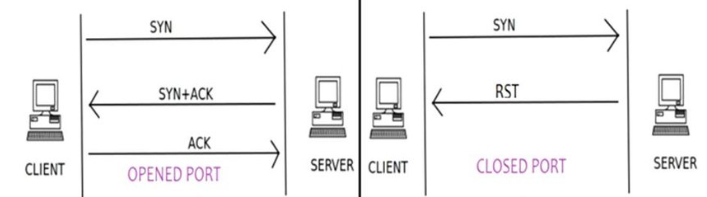
\includegraphics[width=15cm, height=15cm, keepaspectratio]{background/img/open_vs_closed_port.png}
    \caption{Open vs. closed port TCP connection~\cite{Elijla2013}}
    \label{fig:open-vs-closed}
\end{figure}

 Although other TCP header flags, such as FIN (finish), URG (urgent), and PSH (push), can also be utilized by port scanners to identify open ports, SYN scan is the most commonly used technique. This is because it is faster and less likely to be detected by intrusion detection systems (IDS) than other methods. 

\section{Browser-based port scanning vs. Regular Port scanning}

As this paper is focussed on browser-based port scanning, it is important to explain why we make the distinction between regular port scanning and browser-based port scanning. 
There are two major differences, being the type of port scan attacks that we can do, as well as the difference in attack methodology that we employ. 

Regular port scanning is a lot more common, and there are many different types of attacks. The main distinction is that regular port scanning can perform protocol level scans. These type of scans can be very powerful, as small implementation differences at the OS level can be enough to establish a unique fingerprint of a system. In contrast, the scope of browser-based port scanning is defined by the functionality accessible through the abstraction layers of the JavaScript APIs, imposing limitations on its capabilities.

For instance, client-side JavaScript code using the WebSocket protocol cannot create UDP connections, and plain TCP connections cannot be opened either. In order to perform browser-based port scanning, we have to use the abstraction layers that are built on top of the TCP protocol, and leverage JavaScript APIs to send network requests. Figure~\ref{fig:js-network-stack} illustrates this, with the top (blue) layer representing the JavaScript APIs.

\begin{figure}[h]
    \centering
    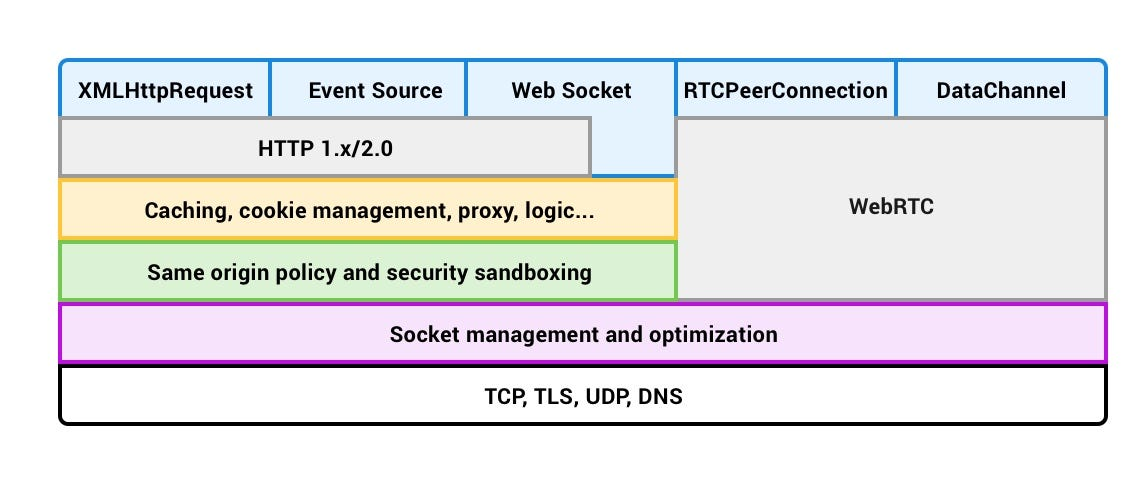
\includegraphics[width=15cm, height=15cm, keepaspectratio]{background/img/js_network_stack.jpg}
    \caption{JavaScript network layer~\cite{medium_js_networking}}
    \label{fig:js-network-stack}
\end{figure}


Aside from the technical scanning capabilities, the attack methodology is different, and this is what makes browser-based port scanning an interesting topic for research. 
Unlike regular port scanning, which embodies an active stance, browser-based port scanning adopts a passive stance. A website can discretely target its visitors without actively probing IPs or initiating network requests. The onus of initiating the attack rests on the user's act of visiting the website. 

The crucial difference between browser-based port scanning and regular port scanning is that a browser-based port scan is executed locally on the user's machine, as opposed to originating from a server. This makes the attack a lot less intrusive, and not as easily detectable by intrusion detection systems. 

The main area of research for browser-based port scanning is the fingerprinting capabilities. 
Browser-based port scanning is limited compared to regular port scanning, and security vulnerabilities are therefore unlikely, as it necessitates a breach of the browser's sandbox environment. For this reason, this paper focuses on privacy vulnerabilities, as ports can reveal a lot of information about the underlying system, and therefore enhance the capabilities of establishing a unique fingerprint.


\section{Ethics and Legality}
Port scanning is a technique that has raised ethical and legal concerns in the past~\cite{jamieson2001}. While some consider it a malicious activity, professionals often use it to identify network problems and detect vulnerabilities in their own network. In the majority of cases, port scanning does not harm the target system, and courts have typically ruled in favor of \\ it~\cite{Lyon2009}.

Recently, the Brandenburg Commissioner for Data Protection (DPA) examined the legality of port scans under GDPR regulations~\cite{gdpr}. In this particular case, port scans were used as a safeguarding mechanism to detect remote access tools such as AnyDesk, Remote Desktop Protocol, and TeamViewer. The DPA ruled in favor of port scanning, deeming it reasonable and understandable with no data protection concerns. This ruling establishes a precedent suggesting that port scanning is permissible under certain circumstances, even though enumerating the entire port range may not be lawful under GDPR~\cite{edpb_decision}.

While cookie consent is commonplace due to GDPR regulations, consenting to a local network search is not. Privacy experts criticized eBay when it was discovered that they had used port scans on the local network of their website visitors. This raises concerns about the lack of consent and transparency surrounding the use of port scanning in such circumstances~\cite{ebay_port_scans}~\cite{forbes_ebay}.

Overall, while port scanning remains a controversial issue, the ruling by the Brandenburg DPA suggests that it can be lawful under certain circumstances. However, it is essential to ensure that individuals are aware of and understand the implications of such scans, particularly when performed without their consent.

\chapter{Related Work}
% You should find out what other researchers have found out about the problem that you will work on. You do that by searching for scientific sources that relate to the problem that you will work on. Often, the chapter in which you wrote your findings is called `Related Work'. Of course, you can choose another title.

% You may conclude this chapter with a subsection in which you show how what you intend to do differs from what has been researched.

% Try to structure this chapter around \emph{subjects} (instead of naming the different authors or articles that you found sequentially). The idea is that you (and your readers) get a clear view on what is known, and what is still unknown with respect to the problem.

% You can, again, start by copying the related work section from your VAF to this chapter. After having done your research (and often during your research) add what you find.


\section{Browser Fingerprinting}
\label{browser-fingerprinting}

Browser fingerprinting is a well-known technique that has garnered significant attention, thanks to Eckersley's pioneering work in bringing the issue to the forefront~\cite{eckersley2010}. Eckersley developed an algorithm capable of identifying a browser fingerprint with an accuracy of 83.6\%, and it could also detect changes in the fingerprint with 99.1\% accuracy. Subsequent studies have focused on exploring various properties that can be utilized for re-identification, including IP address and user-agent~\cite{yen2012}, fingerprinting the HTML5 canvas~\cite{mowery2012}, detection of installed fonts, time zone, and screen resolution~\cite{boda2012}, as well as measuring the timing of the JavaScript engine execution~\cite{mowery2011}~\cite{rokicki2021}, among others.

Nikiforakis et al.~\cite{nikiforakis2013}, Laperdrix et al.~\cite{laperdrix2016} and Gomez et al.~\cite{gomez2018} have further investigated the practical usage of these techniques, showcasing that this is a real threat to user privacy on the internet. Building upon this research, our paper aims to introduce a fingerprinting technique through browser-based port scanning, focusing on an area with limited existing literature.

\section{Fingerprinting running services and the local network}
% Port scanning in general
Aforementioned browser fingerprinting techniques are lacking research when it comes to fingerprinting the local network. Scanning for open ports on the local network can yield promising results, such as revealing running applications on a system.
Port scanning in general is a well-known technique that is widely used due to its utility for network administrators and its potential use by attackers.
% \footnote{\url{https://nmap.org/book/osdetect-methods.html##:~:text=Nmap\%20OS\%20fingerprinting\%20works\%20by,Then\%20Nmap\%20listens\%20for\%20responses}}
Several tools have been developed to scan ports. Nmap~\cite{orebaugh201} is the most popular tool, and the most relevant for this study, because it can fingerprint systems based on port scanning. 

Nmap is a network scanning tool commonly used by network administrators and both ethical and malicious hackers. It comes preinstalled on Kali Linux, a specialized operating system designed for penetration testing. The tool is able to generate a fingerprint of a target system by sending probes to several ports. Nmap uses TCP, UDP and ICMP probes to directly scan for open ports at the protocol level. Various ambiguities in the standard protocol RFC can
then be exploited due to small implementation differences.
Nmap utilizes an extensive fingerprint database to compare the resulting fingerprint with reference fingerprints. See an example reference fingerprint in Figure~\ref{fig:nmap-fingerprint}. 

\begin{figure}[H]
    \begin{verbatim}
    Fingerprint Apple Mac OS X Server 10.2.8 (Jaguar) (Darwin 6.8, PowerPC)
    Class Apple | Mac OS X | 10.2.X | general purpose
    CPE cpe:/o:apple:mac_os_x:10.2.8
    SEQ(SP=FB-111%GCD=1-6%ISR=104-10E%TI=I%II=I%SS=S%TS=1)
    OPS(O1=M5B4NW0NNT11%O2=M5B4NW0NNT11%O3=
    M5B4NW0NNT11%O4=M5B4NW0NNT11%O5=M5B4NW0NNT11%O6=M5B4NNT11)
    WIN(W1=8218%W2=8220%W3=8204%W4=80E8%W5=80F4%W6=807A)
    ECN(R=Y%DF=Y%T=3B-45%TG=40%W=832C%O=M5B4NW0%CC=N%Q=)
    T1(R=Y%DF=Y%T=3B-45%TG=40%S=O%A=S+%F=AS%RD=0%Q=)
    T2(R=N)
    T3(R=Y%DF=Y%T=3B-45%TG=40%W=807A%S=O%A=S+%F=AS%O=M5B4NW0NNT11%RD=0%Q=)
    T4(R=Y%DF=Y%T=3B-45%TG=40%W=0%S=A%A=Z%F=R%O=%RD=0%Q=)
    T5(R=Y%DF=N%T=3B-45%TG=40%W=0%S=Z%A=S+%F=AR%O=%RD=0%Q=)
    T6(R=Y%DF=Y%T=3B-45%TG=40%W=0%S=A%A=Z%F=R%O=%RD=0%Q=)
    T7(R=Y%DF=N%T=3B-45%TG=40%W=0%S=Z%A=S%F=AR%O=%RD=0%Q=)
    U1(DF=N%T=3B-45%TG=40%IPL=38%UN=0%RIPL=G%RID=G%RIPCK=G%RUCK=0%RUD=G)
    IE(DFI=S%T=3B-45%TG=40%CD=S)
    \end{verbatim}
    \caption{Typical Nmap reference fingerprint~\cite{Lyon2009}}
    \label{fig:nmap-fingerprint}
\end{figure}

The example reference fingerprint provides information about an Apple Mac OS X Server 10.2.8 (Jaguar) operating system running on a PowerPC architecture. It includes details about the OS version (10.2.8), the Darwin version (6.8), and the CPE (Common Platform Enumeration) identifier. It also provides information about various scan results, such as open ports (OPS), window size (WIN), ECN (Explicit Congestion Notification) status, and TCP flags (T1-T7). Additionally, it includes details about the IP ID generation (U1) and ICMP error generation (IE) behavior of the system. This technique enables Nmap to detect specific operating systems and versions, including those for embedded systems such as printers running on custom operating systems.

\section{Identifying web automation bots}
As we aim to detect running programs and services on the local network, it is essential to look at existing research on fingerprinting running services. 

Web automation bots such as Selenium~\cite{selenium} are frequently used for large-scale data collection. These bots are susceptible to being detected via fingerprinting techniques, and can be shown different results compared to the original web page. Detecting these bots is a common research topic in browser fingerprinting techniques. Bot detection often involves multiple browser fingerprinting techniques, making it an interesting area of research. 
% Kuchal and Li~\cite{kuchhal2021} show that browser-based port scanning has been used for bot detection in practice. 
Jonker et al.~\cite{jonker2019} reverse engineered a commercial bot detector and discovered several techniques employed in detecting these bots.

\begin{itemize}
    \item Behavior-based web automation bot detection: Multiple event handlers were added to JavaScript events, such as clicks, mouse movements, a device's orientation, motion, keyboard and touch events.
    \item Code injection routines: Frequent communication with the first party server was found. Within this traffic, fingerprinting information was found. This would allow the server to carry out additional server-side bot detection. After identification, bot-specific code can be injected.
    \item DOM properties: Multiple built-in objects and functions were accessed via JavaScript. Additionally, code was found to scan for bot-only properties, such as the \\\verb|document.$cdc_asdjflasutopfhvcZLmcfl_| property --- a property specific to the ChromeDriver.
    This is known by the Chromium team, but currently marked as a \emph{won't fix} issue, stating that if a website owner wants to block automation tools, they respect their decision~\cite{chromedriver_bug}.
    Vlot~\cite{vlot2018} has done extensive research on this, finding several bot-related properties in obfuscated JavaScript files. 
\end{itemize}

Building on top of this research, Krumnow et al.~\cite{krumnow2022} zoomed in on a specific web automation framework, OpenWPM. OpenWPM is a web privacy measurement framework which makes it easy to collect data for privacy studies on a scale of thousands to millions of websites~\cite{openwpm_github}. The research found that OpenWPM was easily detectable and even found OpenWPM detectors in practice. The results indicate that bot detectors are becoming more prevalent, and data obtained through automation frameworks may not be reliable.

% \subsubsection{Website cloaking}
% Cloaking is a technique where different content is presented to different browsers or bots. While it can serve useful purposes such as providing a more accessible version of a website to users with disabilities, it can also be used for unethical practices like hiding negative reviews or for search engine optimization. However, when detected by search engines, this behavior can result in lower rankings and penalties~\cite{cafarella2004}. Furthermore, malicious websites such as phishing sites may use cloaking to avoid detection.



% It is important to distinguish between port scanning in general and port scanning via the browser, because websites may use browser-based scanning to gather information about a user's system without their consent. Although cookie consent is common due to GDPR~\cite{gdpr} regulations, local network search consent is not, and while less common, scanning the local network does occur.

\section{Port scanning via the browser}

Literature on port scanning via the browser is limited. Kuchal and Li~\cite{kuchhal2021} researched how often websites communicate over the local network. They investigated 100k top domains and 145k malware, phishing and abuse websites. The research discovered that hundreds of websites generate requests to the internal network, including websites in the top 10k domains. While not widespread, it is also not trivial. The study found extensive use of WebSockets, in order to bypass the Same-Origin~\cite{w3c_same_origin_policy} policy.

The study identified four primary reasons for local port scanning: fraud detection, bot detection, native application communication, and developer errors. These causes provide insight into the potential of browser-based port scanning and why it is a crucial research topic. Port scanning may be utilized for various purposes, such as fingerprinting for bot and OS detection, preventing remote access tools for fraud detection, and identifying particular application states for native application communication. Native application communication and detecting remote access tools sets browser-based port scanning apart from other fingerprinting methods, because detecting running programs and potentially even specific application states is not possible with regular fingerprinting techniques. Browser-based port scanning may therefore have the ability to take user-tracking to a new level, by profiling users' running programs on their systems. Additionally, port scanning may contribute to existing browser fingerprinting research as it can be used for detecting bots. 

% WEBSOCKET SCANNING: https://incolumitas.com/2021/01/10/browser-based-port-scanning/
% WEBRTC SCANNING: https://medium.com/tenable-techblog/using-webrtc-ice-servers-for-port-scanning-in-chrome-ce17b19dd474

% Web bot detection techniques.

% Website cloaking.

% Fingerprint-detection scanners.

% Port scanning

% \templateinfo{
% You should find out what other researchers have found out about the problem that you will work on. You do that by searching for scientific sources that relate to the problem that you will work on. Often, the section in which you wrote your findings is called `Related Work'. Of course, you can choose another title.

% You may conclude this section with a subsection in which you show how what you intend to do differs from what has been researched.

% Try to structure this section around \emph{subjects} (instead of naming the different authors or articles that you found sequentially). The idea is that you (and your readers) get a clear view on what is known, and what is still unknown with respect to the problem.
% }

% ==========================================================================
\chapter{Estimating the optimal port scanning technique}
\label{chapter:scanning-techniques-experiment}
% ==========================================================================

In this chapter, we present the results of three experiments that were conducted to estimate the most effective browser-based port scanning strategy for several combinations of operating system and browser. 
The first experiment focuses on estimating the optimal socket timeout setting, this experiment focuses on finding a balance between efficacy and efficiency.
The second experiment focuses on estimating the most effective scanning technique, this experiment focuses on the capability of JavaScript APIs to detect open ports.
The third experiment focuses on estimating the most efficient scanning technique, this experiment focuses on parallel connections.

\section{Definitions}

In order to address RQ1 effectively, it is crucial to establish clear definitions for attack goals, efficiency, and efficacy.

\subsubsection{Attack goals}

Attack goals refer to the specific objectives that an attacker aims to achieve by scanning ports. Generally, there are two common attack goals:

\begin{enumerate}[label=\alph*.]
    \item Enumerating the entire port range: This goal involves scanning all available ports on a target system to gather comprehensive information about its open and closed ports. It allows the attacker to obtain a broad understanding of the target's network services and potential vulnerabilities.
    
    \item Scanning for a specific number of ports: In this case, the attacker focuses on scanning a limited number of ports that are of particular interest. This targeted approach enables them to gather specific information related to those ports or services. It represents a trade-off between scanning for precise information and maximizing the amount of information gathered.
\end{enumerate}

It is worth noting that certain scanning techniques may be required to detect specific ports effectively, depending on the attack goals.

\subsubsection{Efficacy}

Efficacy is closely tied to the attack goal. 
It signifies the degree to which a scan successfully accomplishes its intended objective. 
The efficacy of a scan depends on whether the desired information can be obtained from one or more targeted ports.

For instance, if the attacker is scanning for a specific port, they may employ techniques tailored to detecting that port accurately. If the desired information can be retrieved from the scanned port(s), the scan is considered efficacious.

\subsubsection{Efficiency}

Efficiency is determined by various factors that impact the time and resources required to complete a scan. These factors include:

\begin{enumerate}[label=\alph*.]
    \item Number of parallel sockets: The number of parallel sockets running simultaneously during the scan affects how many ports can be scanned concurrently. Increasing the number of parallel sockets generally improves scan speed.
    
    \item Socket timeouts: Socket timeouts determine the duration for which the scanning tool waits for a response from each port. Optimal timeout settings balance the time required for accurate detection against minimizing delays.
    
    \item Number of scans to be executed: The number of scans an attacker intends to perform can impact efficiency. Performing multiple scans may be necessary to gather comprehensive information or increase the chances of successfully detecting specific ports.
    
    \item Additional overhead: Various factors such as browser, operating system, and hardware configurations can introduce overhead during the scanning process. These should be taken into account when evaluating efficiency.
\end{enumerate}

Efficiency is commonly assessed based on the time required to complete a scan. The faster a scan can be accomplished without compromising the desired efficacy, the more efficient it is considered. 


\section{Background}

This section provides an overview of potential scanning techniques that were considered for the experiment. Due to the constraints imposed by the abstraction layers provided by JavaScript APIs, the options are limited, every available JavaScript API capable of performing network requests was considered.

\subsection{Scanning techniques overview}
\subsubsection{Fetch API}

The Fetch API is a modern JavaScript API that provides an interface for making asynchronous HTTP requests. It allows us to send HTTP(S) requests to a specified URL and handle the responses. The Fetch API offers a more powerful and flexible alternative to the traditional XMLHttpRequest (XHR) approach.

\subsubsection{XMLHttpRequest (XHR)}

XMLHttpRequest is a JavaScript API that has been widely used for making asynchronous HTTP requests. It provides a way to send HTTP(S) requests to a server and receive responses. Although Fetch API is gaining popularity, XHR is still supported in most browsers and can be used for network requests.

\subsubsection{WebSocket}

WebSocket is a communication protocol that provides full-duplex communication channels over a single TCP connection. It enables real-time, bidirectional communication between a client and a server. WebSocket API in JavaScript allows establishing WebSocket connections and exchanging data between the client and the server.

% Below scanning techniques were considered, but deemed to be impossible to be used as a port scanning technique after conducting some experiments. These techniques can \emph{send} a stream of data over the network, but do not necessarily expect a response. It is therefore impossible to detect if a service might be running on a port using these scanning techniques.

\subsubsection{WebRTC}

WebRTC (Web Real-Time Communication) is a collection of communication protocols and APIs that enables peer-to-peer audio, video, and data sharing between browsers. It allows direct communication between browsers without the need for intermediate servers. WebRTC API provides methods to establish connections, exchange data, and control media streams.
WebRTC used to be a viable port scanning technique in the past, due to the \texttt{RTCPeerConnection.onicecandidateerror} event handler emitting useful error information about the status of the connection. However, after being exploited by Baines~\citearticle{baines2019} in 2019, 
this functionality has been removed for local connections~\citeartifact{webrtc}, and therefore scanning the local network via WebRTC is not possible anymore.

\subsubsection{Beacon API}

The Beacon API is a lightweight and efficient API for sending small amounts of data to a server asynchronously. It is designed for sending analytics data or other non-critical information without delaying or blocking the loading of the next page. The Beacon API is designed so that it can only \emph{send} data to a server, but not retrieve any. Therefore, we cannot use this API to determine the status of a port.

\subsubsection{Server-Sent Events}

Server-Sent Events (SSE) is a server push technology that enables continuous updates from the server to the client over a single HTTP(S) connection. However, SSE cannot be used for port scanning purposes due to its inherent design limitations. SSE operates on an event-driven model, where the server sends events to the client asynchronously. As SSE only allows data to flow from the server to the client and does not support client-initiated requests, it lacks the necessary functionality for conducting port scanning.

% ==========================================================================
\subsubsection{Scanning techniques comparison}
% ==========================================================================

The aforementioned JavaScript APIs leaves us with three possible APIs to perform browser-based port scanning: Fetch, XHR and WebSockets. As all three APIs are built on top of the TCP protocol, this limits the potential results that may be achieved, as the status of UDP ports will remain undetectable. 

While Fetch and XHR are similar in functionality, WebSockets are not built on top of the HTTP protocol, and could therefore achieve different results. WebSocket and HTTP are separate protocols that operate at layer 7 in the OSI model~\citescientific{kumar2014} and rely on TCP at layer 4. However, despite their differences, RFC 6455~\citetechnical{fette2011} specifies that WebSocket `is intended to be compatible with HTTP-based server-side software and intermediaries'. This compatibility is achieved through the WebSocket handshake, which utilizes the HTTP Upgrade header to transition from the HTTP protocol to the WebSocket protocol.
% This suggests that the WebSocket API could be the most effective scanning technique, as it is able to make requests over both the WebSocket and the HTTP protocol.

% ==========================================================================
\section{Experiment Setup}
% ==========================================================================

Having established the availability of three scanning techniques via the XHR, Fetch, and WebSocket APIs, we created an experiment to compare these techniques based on several metrics.

\subsection{Application design}
\label{section:port-scanner-application}

A client-side TypeScript web application was developed to facilitate a comparative analysis of these three JavaScript APIs. The application's design was guided by specific considerations outlined below, aimed at optimizing its functionality and applicability for forthcoming chapters.

Central to the application's design is the incorporation of configurability features. These features encompass essential parameters such as socket timeout, parallel socket connections, and the scanning technique. The rationale behind this emphasis on configurability lies in the necessity to ensure uniformity and consistency across various scans during the experiment. By maintaining consistent settings, the application enables accurate and meaningful comparisons between different scanning approaches.

These settings can be passed to the application using query parameters, as depicted in Figure~\ref{fig:initiate-scan}. 

\begin{figure}[ht]
    \centering
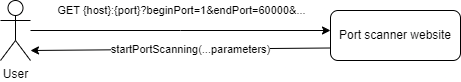
\includegraphics[width=10cm, height=10cm, keepaspectratio]{port_scanning_techniques/img/initiate_port_scan.png}
    \caption{User initiating port scan}
    \label{fig:initiate-scan}
\end{figure}

Upon requesting the webpage, a JavaScript file will be returned which initiates a scan on the localhost IP address. The available query parameters are listed in Table~\ref{tab:port-scan-params}. This solution was chosen to make the scans scriptable and therefore easily useable with automation frameworks such as Selenium.

\begin{table}[htbp]
\footnotesize
\centering
% \begin{adjustwidth}{-0.5cm}{}
\begin{tabular}{p{3cm} p{10cm}}
    \toprule
    Parameter & Description \\
    \midrule
    beginPort & The starting port for the scanning range. \\
    endPort & The final port for the scanning range. Scanning will be performed within the range from beginPort to endPort. \\
    nScans & The number of scan iterations for each individual port. For example, if nScans=10, each port within the specified range will be scanned 10 times. \\
    nSockets & The maximum number of sockets used for concurrent parallel scanning. \\
    socketTimeout & The time limit for a single scan attempt on a port. If the scan doesn't complete within this timeframe, the scanner aborts the scan and moves to the next port. \\
    scanningTechnique & The selected method for performing scans, such as fetch, xhr, or websockets. \\
    \bottomrule
\end{tabular}
% \end{adjustwidth}{}
\caption{Port scanner application available query parameters}
\label{tab:port-scan-params}
\end{table}

Existing client-side port scanning applications often share a common limitation known as batch-job scanning. In this approach, a predefined range of ports, such as ports 1-50, is scanned concurrently based on a configured parallel sockets count (referred to as "nSockets" in Table~\ref{tab:port-scan-params}). All ports within this designated range are scanned simultaneously within a batch. After completing the entire batch, the scanning process proceeds to the subsequent batch. However, this method suffers from inefficiencies due to variations in the time it takes to scan different ports. Consequently, there's a reduced number of parallel sockets, typically less than 50, actively operating at any given time. This limitation hampers the overall efficiency of the scanning process.

To overcome this limitation, we have created a queuing mechanism designed to eliminate this limitation and ensure optimal utilization of parallel sockets throughout the scanning process. This queuing system operates on the principle of promptly dequeuing a scanning job once the scan of a port is completed. By adopting this approach, our application guarantees a consistent and maximum utilization of parallel sockets throughout the entire scanning operation. This queuing mechanism optimally distributes scanning tasks, minimizing idle periods, and thereby significantly enhancing the efficiency of the scanning process.

This improvement is illustrated by comparing the two techniques in Figures~\ref{fig:batch-job} and~\ref{fig:queue-job}. The comparison visually demonstrates port scans on six ports, with three scans concurrently executed in parallel. In this hypothetical scenario, a reduction of 100ms in scanning time is simulated. While this incremental gain might seem minor when scanning a limited number of ports, say 1000, its impact becomes notably significant when extending the scope of the scan to encompass the entire port range, spanning from 0 to 65536.

\begin{figure}[htbp]
    \centering
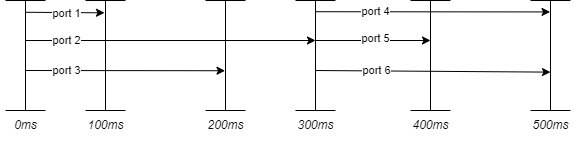
\includegraphics[width=10cm, height=10cm, keepaspectratio]{port_scanning_techniques/img/batch-job.jpg}
    \caption{Batch-job scanning}
    \label{fig:batch-job}
\end{figure}

\begin{figure}[htbp]
    \centering
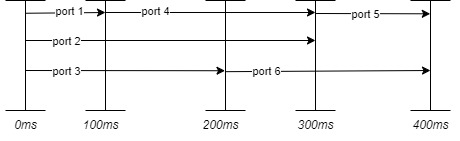
\includegraphics[width=10cm, height=10cm, keepaspectratio]{port_scanning_techniques/img/queue-job.jpg}
    \caption{Queueing jobs concurrently}
    \label{fig:queue-job}
\end{figure}

By adopting the queuing mechanism, our approach mitigates the inefficiencies inherent in batch-job scanning, leading to a substantial improvement in the efficiency and speed of port scanning, particularly when dealing with a larger range of ports.

When all ports have finished scanning, the results of the scan are posted back to the server for post-scan analysis. The implementation of the full application can be found on GitHub~\citeartifact{bvdl2023}

\subsection{Docker Containerization}
\label{section:experiment-setup}

In order to conduct our experiments systematically and ensure reproducibility, we employed a fully automated approach utilizing Docker containers. This approach encapsulated the entire experiment, maintaining consistency and facilitating the ability to replicate the experiments precisely. The setup was designed to be repeatable by others and consisted of the following key components:

We employed Docker containers to establish a self-contained and isolated environment for conducting our experiments. This approach effectively eliminated potential issues that could arise from variations in the underlying host systems.

The use of Docker containers provided us with the capability to define and manage various experiment parameters, including operating systems, web browsers, socket settings, and scanning techniques, all through Dockerfiles. This ensured that the experiment environment remained consistent and reproducible across multiple runs.

Within these Docker containers, we included servers that served as potential attack targets. Among them, there is a server that hosts an implementation of the browser-based port scanning application, simulating a website running browser-based port scanning attacks. Furthermore, our Docker containers also contain a client-side Selenium application responsible for initiating and interacting with the browser-based port scanning application during the experiments, utilizing headless browsers.

\subsubsection{Automated Scripting}

We developed automated scripts to orchestrate and execute the experiments within the Docker containers. These scripts facilitated the setup and execution of the scans, with precise control over the scanning parameters.
The automation enabled us to easily run multiple experiments in a scripted manner, ensuring accurate and reproducible results.

\subsubsection{Data Collection Metrics}

Throughout the experiments, we systematically gathered data with a focus on two key metrics: efficacy and efficiency.

\begin{itemize}
    \item \textbf{Efficacy} was defined by the count of accurately identified open ports.
    \item \textbf{Efficiency} was evaluated by analyzing the speed of the scanning process while ensuring that the efficacy of port detection remained uncompromised.
    \item For each scan, we collected the following metrics:
    \begin{itemize}
        \item A timestamp indicating when the scan started and ended.
        \item The port number and its status (open/closed).
        \item Start and end times of each individual port scanned.
    \end{itemize}
    \item Additionally, post-scan analysis was employed to determine port status via timing measurements.
\end{itemize}

\subsubsection{Experiment Reproducibility}
\begin{itemize}
    \item To ensure the reproducibility of the experiments, we shared Docker images and scripts used for the experiments, allowing other researchers to replicate our setup easily.
    \item The encapsulation and isolation provided by Docker containers guaranteed a consistent experiment environment, irrespective of the host system's variations.
\end{itemize}

The utilization of Docker containers for our experiments effectively addressed the challenges related to reproducibility in scientific research. The experimental setup is visually represented in Figure~\ref{fig:experiment}.

\begin{figure}[tbh]
    \centering
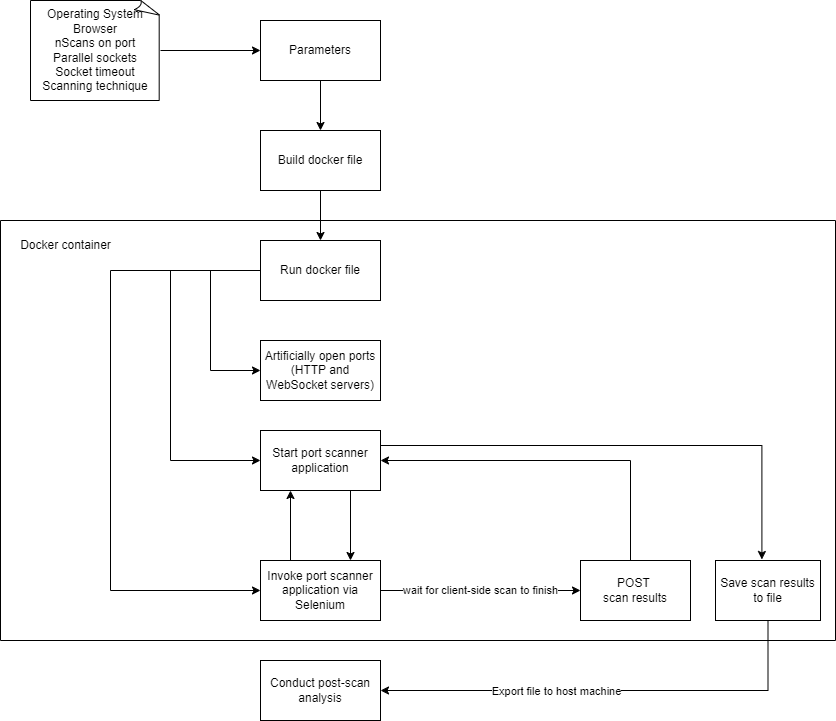
\includegraphics[width=15cm, height=15cm, keepaspectratio]{port_scanning_techniques/img/portscan_experiment.png}
    \caption{Experiment setup}
    \label{fig:experiment}
\end{figure}


% Besides this queueing mechanism, we implemented an abstraction layer which enables us to pass a different scanning function (XHR, Fetch, WebSocket) without having to make functional changes to the underlying logic. The only difference in logic is the scanning technique implementation. The implementation of the port scanner application can be found on GitHub~\cite{bvdl2023}

% \section{Experiments}

% Three experiments were conducted to estimate the optimal browser-based port scanning. The overarching objective of these experiments was to discern the most suitable port scanning technique for each unique combination of operating system and browser. This discernment serves as a foundation for subsequent chapters, wherein deeper exploration into the capabilities of browser-based port scanning is undertaken.

\section{Experiment 1: Estimating the optimal socket timeout setting}
\label{section:socket-timeout-setting}

In the context of browser-based port scanning, there are two key motivations for considering the adjustment of the socket timeout setting:
\subsection{Motivation}
\subsubsection{Enhancing Scan Efficiency}

One primary motivation for altering the socket timeout setting is to improve the efficiency of the port scanning process. This involves two key aspects:

\begin{itemize}
  \item \textbf{Faster Scanning}: By lowering the socket timeout, the scanner spends less time waiting for responses from each port. Consequently, this leads to quicker scans, as the scanner can move on to the next port faster.

  \item \textbf{Efficiency Gains}: Ultimately, the objective is to achieve higher overall efficiency, enabling the scanning of more ports within a shorter time frame. This is particularly important when conducting large-scale or time-sensitive scans.
\end{itemize}

\subsubsection{Balancing Efficacy and Speed}

While efficiency gains are desirable, there is an inherent trade-off between scan speed and efficacy when adjusting the socket timeout setting:

\begin{itemize}
  \item \textbf{Efficacy Concerns}: Setting the socket timeout too low might result in inaccurate scan results. In such cases, the scanner may not wait long enough to receive a response from the target port, potentially leading to false negatives.

  \item \textbf{Finding the Optimal Balance}: Therefore, it becomes crucial to strike a balance between efficacy and efficiency. The challenge lies in identifying the lowest socket timeout value that maintains efficacy without sacrificing scan efficiency.
\end{itemize}

\subsection{Experiment Target}

In order to address the motivations outlined above, the experiment targets the following objectives:

\subsubsection{Determining the Optimal Socket Timeout}

\begin{itemize}
  \item \textbf{Objective}: The primary objective of the experiment is to identify the socket timeout value that strikes the ideal balance between scan speed and efficacy.
  
  \item \textbf{Analysis of Results}: Data collected during the experiment is analyzed comprehensively to determine which socket timeout setting achieves this balance most effectively.
  
  \item \textbf{Validation}: The identified optimal socket timeout value is further validated by conducting additional scans on different target systems. This validation step ensures that the selected setting is applicable and reliable across various scanning scenarios, providing a robust solution for future port scanning endeavors.
\end{itemize}

\subsubsection{Socket Timeout Adjustment}

\begin{itemize}
  \item \textbf{Socket Timeout Setting}: The primary variable under investigation in this experiment is the socket timeout setting.
  
  \item \textbf{Range of Values}: The experiment involves testing a range of socket timeout values, spanning from very low settings to moderate values.
  
  \item \textbf{Measurement of Efficiency}: Efficiency in this context is quantified by measuring the time taken to complete the port scan for each tested socket timeout value.
  
  \item \textbf{Measurement of Efficacy}: To assess efficacy, the scan results are compared against a reference set of known open and closed ports.
\end{itemize}

The parameters for the experiments can be found in Appendix~\ref{appendix:expirement-parameters}. 
We chose not to include MacOS in the list of Operating Systems because of compatibility issues with Docker.


% \subsection{Experiment Setup}

% The automated setup as outlined in Section~\ref{section:experiment-setup} was used for the experiment. Several Docker images were created using different operating systems, browsers, and socket timeout settings. These parameters are listed in Appendix~\ref{appendix:expirement-parameters}.

\subsection{Experiment Results}

In this experiment, we investigated the impact of varying socket timeout settings on the efficacy and efficiency of port scanning using different web browsers and operating systems. The key findings are summarized below:

\subsubsection{Socket Timeout Settings and Efficacy}

We observed that the choice of socket timeout setting significantly affected the efficacy of port scanning, particularly for the Chrome and Firefox browsers. Specifically:

\begin{itemize}
    \item \textbf{Chrome Browser}:
    \begin{itemize}
        \item Using a socket timeout of 100 milliseconds resulted in reduced efficacy, with 76 ports being detected rather than the configured 100 open ports.
        \item The efficacy reached 100\% when a socket timeout setting of 150ms was used.
    \end{itemize}
    
    \item \textbf{Firefox Browser}:
    \begin{itemize}
        \item Similar outcomes were measured for Firefox, with a timeout of 100 milliseconds resulting in only 21 detected ports.
        \item The efficacy reached 100\% when a socket timeout setting of 150ms was used.
    \end{itemize}
\end{itemize}

The raw results can be found in Appendix A, Table~\ref{tab:socket-timeout-comparison}.

\subsubsection{Real-world Validation}

To ensure the reliability of our findings, we conducted real-world validation of the results obtained within our virtualized environment. The validation process revealed interesting insights:

\begin{itemize}
    \item \textbf{Chrome's Consistency}: After validating the results in a real-world scenario, Chrome's efficacy remained consistent at 100\% with a 150ms timeout, reinforcing the reliability of this setting.
    
    \item \textbf{Firefox's Variable Performance}: In contrast, Firefox's results were inconsistent until a timeout of 400ms was used in a real-world context. This variability highlights the importance of considering real-world scenarios in setting optimal socket timeouts.
\end{itemize}


\subsubsection{Socket Timeout Behavior in Different Operating Systems}
\label{section:socket-timeout-comparison}

In our experiments, we observed a notable difference in how socket timeout settings are handled by different operating systems.

\begin{itemize}
    \item \textbf{Windows Operating System}:
    \begin{itemize}
        \item Windows respects the configured socket timeout setting as defined in the scanning parameters.
        \item The efficacy and timing of port responses closely align with the specified timeout, making the socket timeout setting a critical factor in scan efficacy and efficiency on Windows.
    \end{itemize}
    
    \item \textbf{Ubuntu Operating System}:
    \begin{itemize}
        \item In contrast, Ubuntu exhibits a distinct behavior. The operating system ignores the configured timeout and automatically times out the request when possible.
        \item Ports generally respond within a range of 5--75 milliseconds on Ubuntu, irrespective of the configured socket timeout setting.
        \item This behavior makes socket timeout settings less critical on Ubuntu, as the automatic request timeout mechanism often results in responses occurring well within the specified timeout.
    \end{itemize}
\end{itemize}


\subsection{Analysis}

The socket timeout settings play a pivotal role in determining the efficacy and efficiency of browser-based port scanning.

\begin{enumerate}
    \item \textbf{Chrome Browser}: A socket timeout setting of 150ms consistently achieves 100\% efficacy in both virtualized and real-world environments. It strikes an optimal balance between efficacy and speed for Chrome.
    \item \textbf{Firefox Browser}: A longer timeout of 400ms is advised for Firefox, as we measured that the optimal socket timeout of 150ms during our testing was not accurate during real-world validation. This difference can be attributed to the headless Firefox browser used in our experiments, which is considerably more efficient than the regular browser used in real-world scanning scenarios.
    \item \textbf{Ubuntu Operating System}: Ubuntu's automatic request timeout mechanism minimizes the influence of socket timeout settings. Responses generally occur within 5-75ms, making precise tuning of the socket timeout setting less critical. 
    \item \textbf{Windows Operating System}: On Windows, socket timeout settings have a more pronounced impact. The operating system respects the configured socket timeout setting, leading to a loss of efficacy in the scan results when the socket timeout is too low. 
\end{enumerate}

\subsubsection{Conclusion}

In the context of browser-based port scanning, adjusting the socket timeout setting serves two key purposes:

\begin{enumerate}
    \item \textbf{Efficiency Improvement}: Lowering the socket timeout accelerates scanning, enhancing efficiency for large-scale or time-sensitive scans.
    \item \textbf{Balance between Efficacy and Efficiency}: Striking the right balance between efficacy and efficiency is crucial. An overly low timeout compromises efficacy, while a very high timeout compromises efficiency.
\end{enumerate}

Our experiments recommend a socket timeout of 150ms for Chrome and 400ms for Firefox. These settings ensure efficient scans on both Windows and Ubuntu while maintaining a 100\% detection rate of open ports. It is worth noting that Ubuntu's automatic request timeout mechanism minimizes the influence of socket timeout settings, making precise tuning less critical on this operating system.

\section{Experiment 2: Estimating the most effective scanning technique}

\subsection{Motivation}

\begin{itemize}
    \item \textbf{Efficacy}: The motivation behind this experiment is to identify the most effective scanning technique for browser-based port scanning.
    \item \textbf{Comparing scanning techniques}: The goal is to determine which of the three scanning technique -- Fetch, XHR (XMLHttpRequest), and WebSocket APIs -- offers the highest efficacy in detecting open ports.
\end{itemize}

\subsection{Experiment Target}

The experiment is designed to investigate and compare the efficacy of different scanning techniques, namely the Fetch, XHR and WebSocket APIs.

The experiment targets the following specific objectives:
\begin{itemize}
    \item Evaluate the efficacy of each scanning technique in detecting open ports using the intended functionality of the APIs.
    \item Evaluate the efficacy of each scanning technique in detecting open ports using a timing attack method.
\end{itemize}


% \subsection{Experiment Setup}

% The automated setup as outlined in Section~\ref{section:experiment-setup} was used for the experiment. Several Docker images were created using different operating systems, browsers, and different attack targets (servers representing attack objectives), These parameters are listed in Appendix A~\ref{appendix:experiment-parameters}.

\subsection{Experiment Results}

In this experiment, we evaluated the efficacy of three scanning techniques –- the Fetch, XHR, and WebSocket APIs –- with the optimal socket timeout setting determined in the previous experiment. The raw results can be found in Table~\ref{tab:scan-technique-comparison}.

\subsubsection{Fetch API Outperforms}

\begin{itemize}
    \item The Fetch API demonstrated superior performance, achieving a 100\% open port detection rate.
    \item This success can be attributed to its unique ability to operate in the \emph{no-cors} mode within JavaScript, allowing cross-domain requests, including requests to localhost, without CORS restrictions.
\end{itemize}

\subsubsection{XHR and WebSocket with Post-Scan Analysis}

\begin{itemize}
    \item Initially, both the XHR and the WebSocket APIs struggled to detect open ports and exhibited a 0\% detection rate using the intended functionality of the respective APIs.
    \item However, post-scan analysis revealed their potential by comparing response times between closed and open ports. Ports responding within less time than the configured socket timeout were consistently found to be open on the Windows operating system.
    \item The timing attack method was not applicable on the Ubuntu operating system due to response times being similar between open and closed ports.
\end{itemize}

Particularly on the Windows operating system, the XHR and WebSocket  detection capabilities were significantly enhanced when utilizing this timing attack method, enabling the XHR API to achieve a 100\% open port detection rate. This is depicted in Figures~\ref{fig:win-chrome-xhr} and~\ref{fig:win-firefox-xhr}.

\begin{figure}[ht]
\centering
\begin{minipage}{.45\textwidth}
  \centering
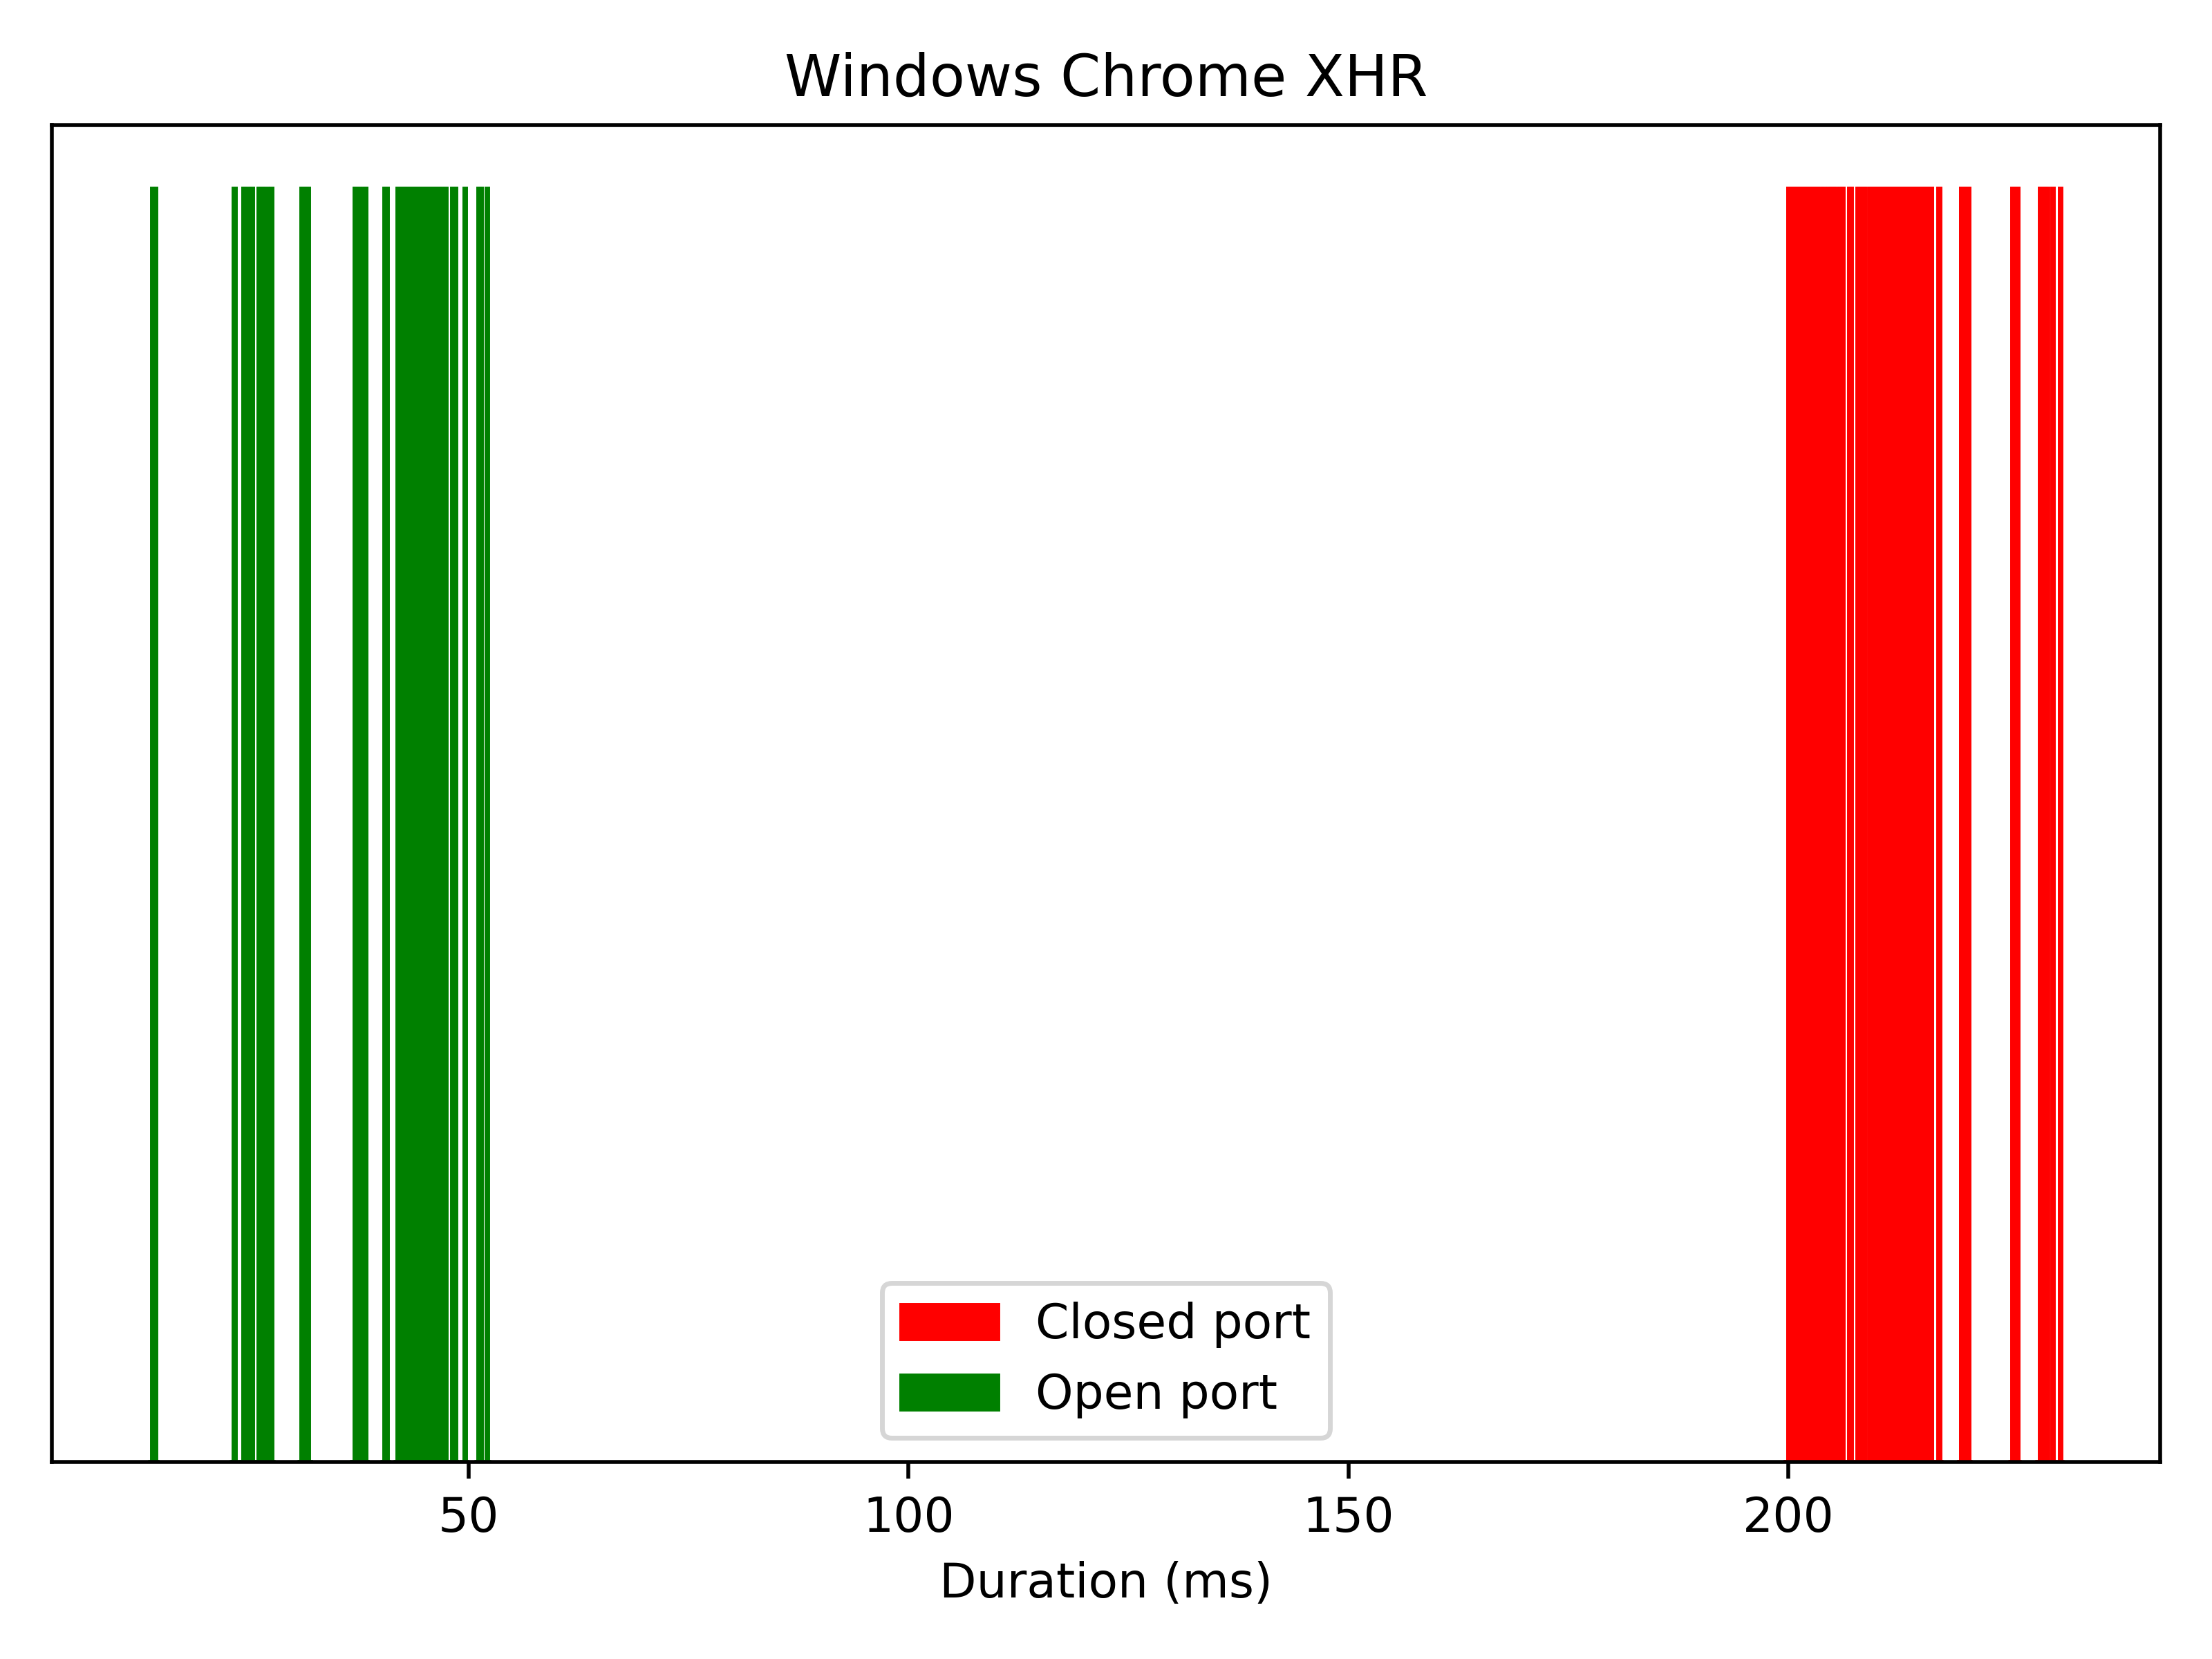
\includegraphics[width=10cm, height=5cm, keepaspectratio]{port_scanning_techniques/img/windows_chrome_efficacy_xhr.png}
    \caption{Windows/Chrome XHR API scan duration open vs closed ports}
    \label{fig:win-chrome-xhr}
\end{minipage}
\hspace{0.5cm} % Adjust the horizontal space between the two figures
\begin{minipage}{.45\textwidth}
\includegraphics[width=10cm, height=5cm, keepaspectratio]{port_scanning_techniques/img/windows_firefox_efficacy_xhr.png}
    \caption{Windows/Firefox XHR API scan duration open vs closed ports}
    \label{fig:win-firefox-xhr}
\end{minipage}
\end{figure}

The combination of WebSocket/Firefox also had an increased detection rate of 100\%, but WebSocket/Chrome remained unable to detect any of the open ports, this is depicted in Figures~\ref{fig:win-firefox-websocket} and~\ref{fig:win-chrome-websocket}. Further comparisons can be found in Appendix A, Section~\ref{appendix:scan-duration-comparison}

\begin{figure}[ht]
\centering
\begin{minipage}{.45\textwidth}
  \centering
\includegraphics[width=8cm, height=4cm, keepaspectratio]{port_scanning_techniques/img/windows_Firefox_efficacy_websocket.png}
    \caption{Windows/Firefox WebSocket API scan duration open vs closed ports}
    \label{fig:win-firefox-websocket}
\end{minipage}
\hspace{0.5cm} % Adjust the horizontal space between the two figures
\begin{minipage}{.45\textwidth}
  \centering
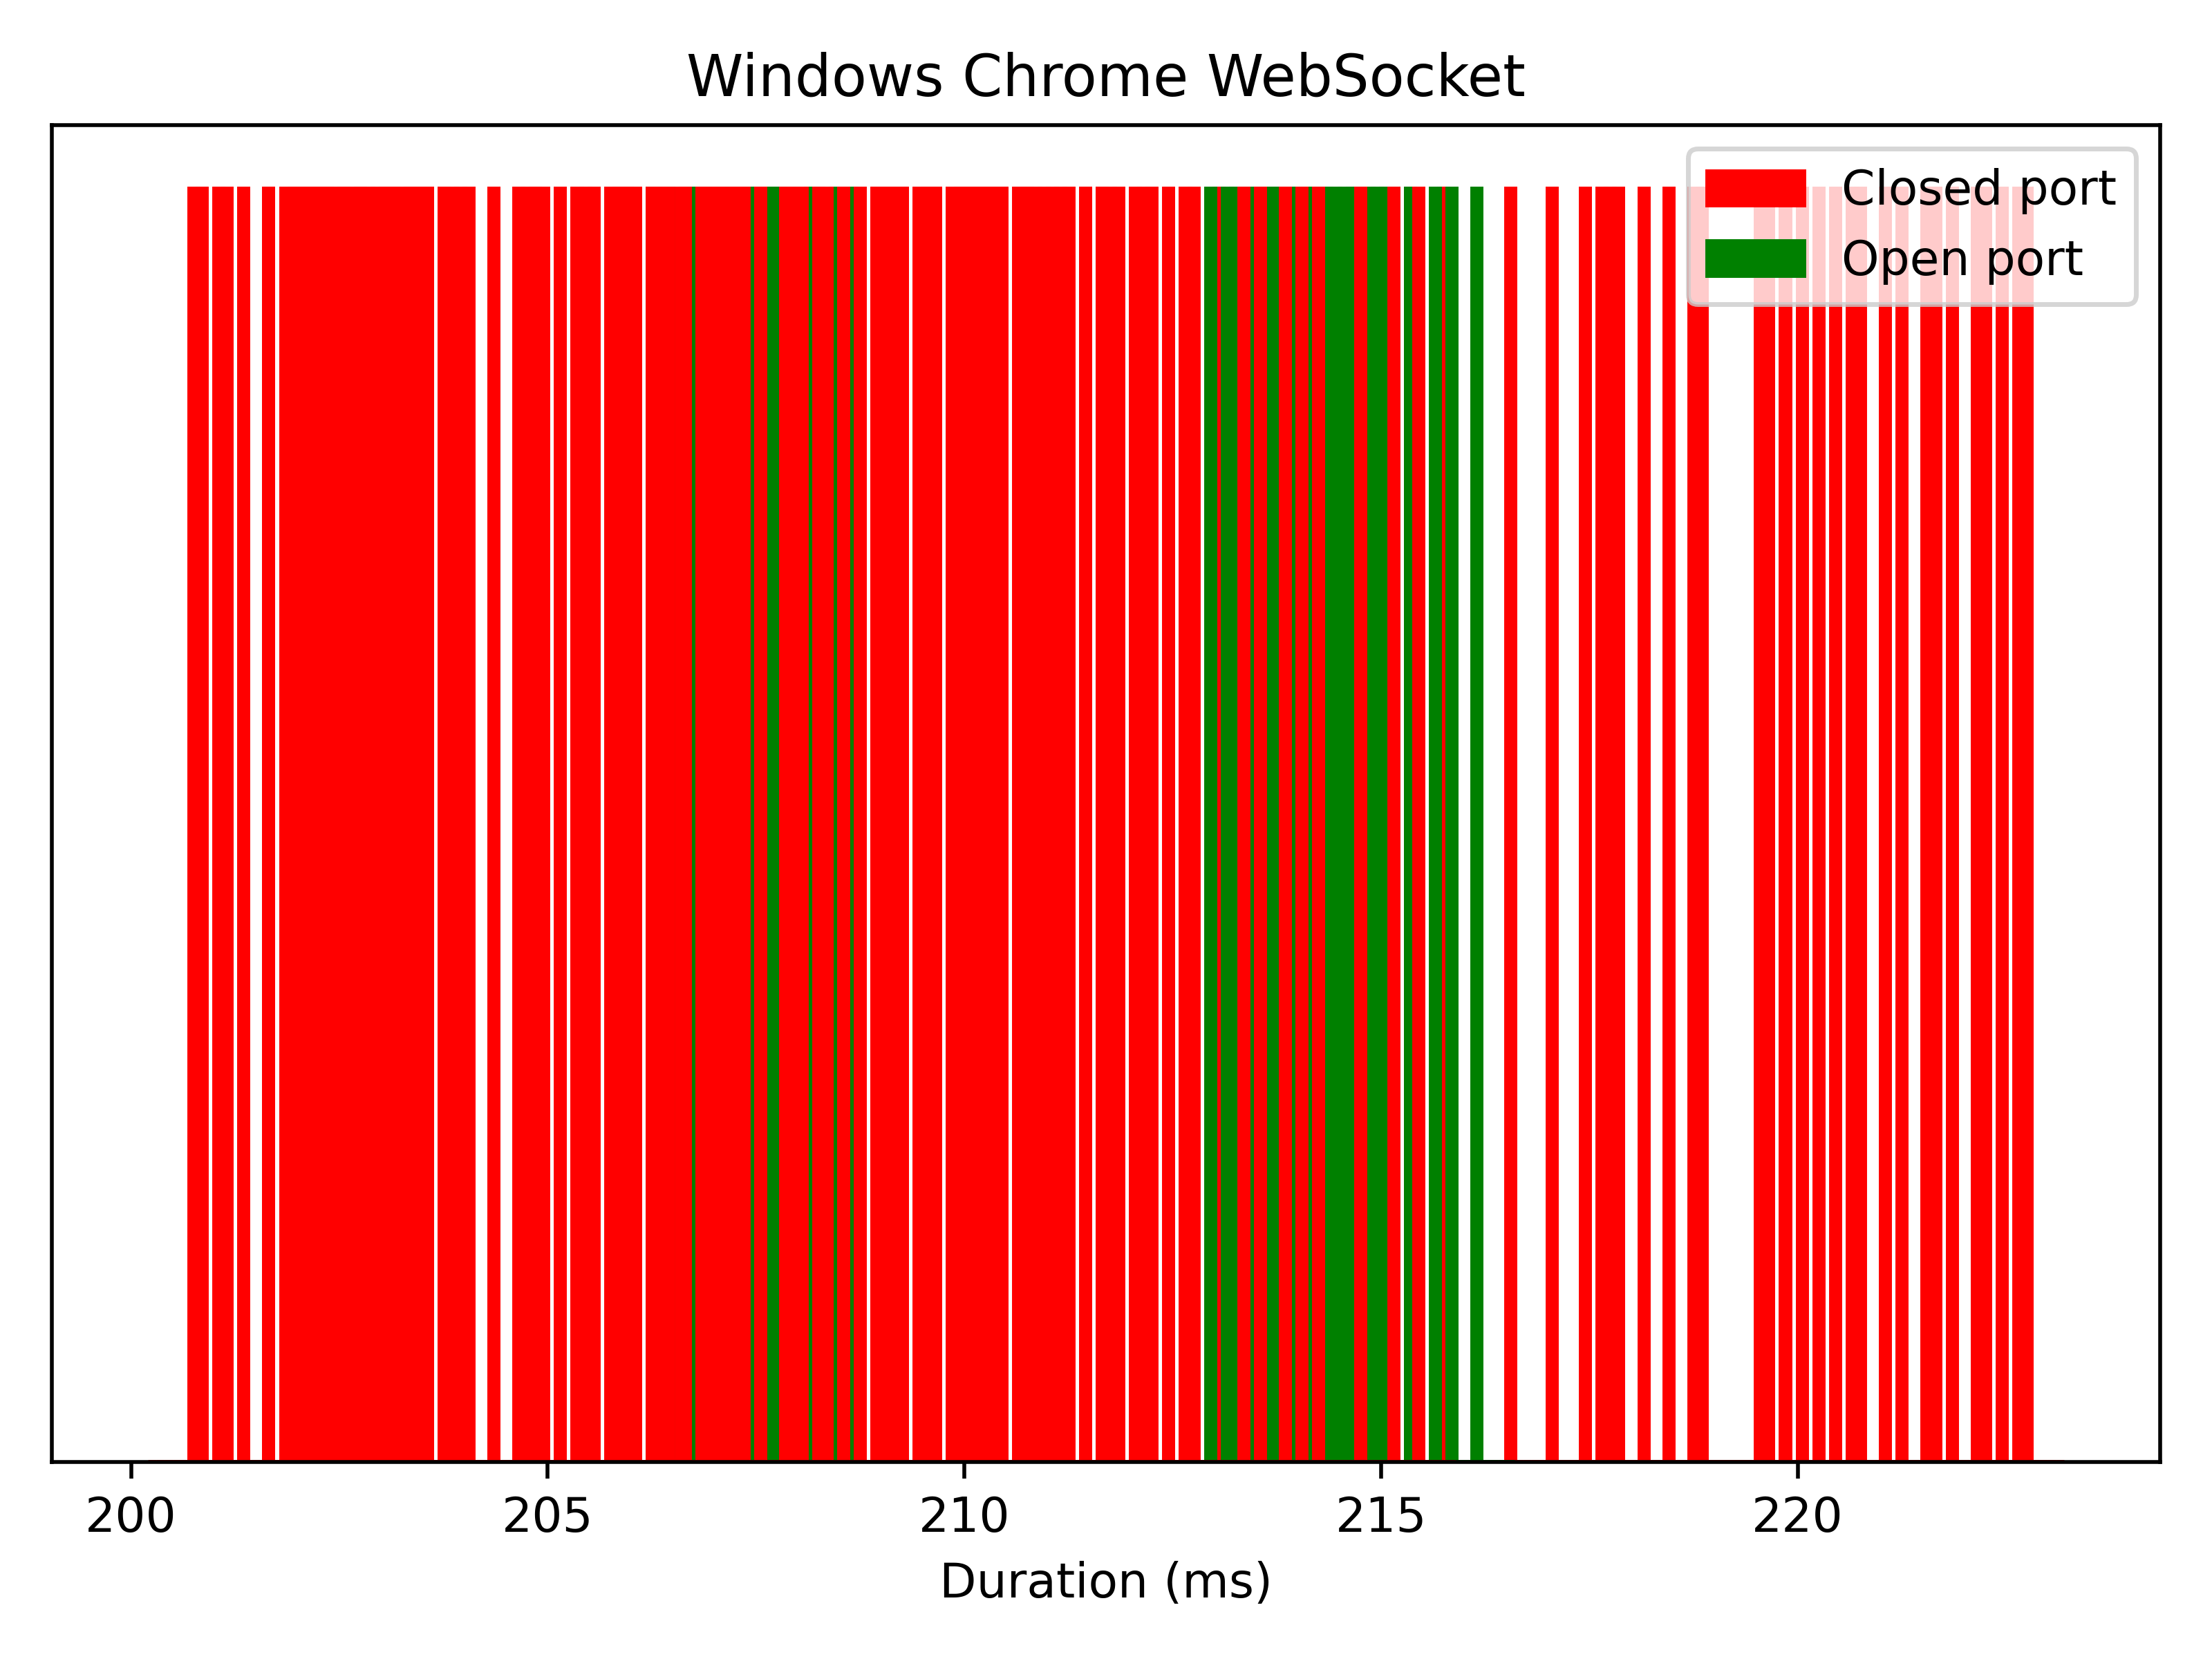
\includegraphics[width=8cm, height=4cm, keepaspectratio]{port_scanning_techniques/img/windows_chrome_efficacy_websocket.png}
    \caption{Windows/Chrome WebSocket API scan duration open vs closed ports}
    \label{fig:win-chrome-websocket}
\end{minipage}
\end{figure}

\subsection{Analysis}

\subsubsection{Fetch API Advantage}

\begin{itemize}
    \item The Fetch API's success lies in its \emph{no-cors} mode, allowing it to bypass CORS restrictions and reliably detect open ports.
    \item Despite limitations in this mode, such as restricted headers and inability to access response details, the Fetch API is able to reliably determine open HTTP ports using this method.
\end{itemize}


\subsubsection{XHR and WebSocket Potential}

\begin{itemize}
    \item While XHR and WebSocket APIs initially struggled to detect any open ports using their native API functionality, however, post-scan analysis utilizing response time measurements unveiled their potential.
    \item The timing attack method significantly enhanced their performance on Windows systems, achieving a 100\% open port detection rate.
    \item However, the absence of a clear response time distinction between open and closed ports on Ubuntu limits the applicability of this method.
\end{itemize}

\subsubsection{Consideration of Unsafe Ports}

The presence of \emph{unsafe} ports~\citetechnical{firefox_restricted_ports}\citeartifact{chrome_restricted_ports}, which cannot be reliably classified as open or closed, introduces complexity to port scanning.
Unsafe or restricted ports refer to a range of TCP/UDP ports that are reserved for system or administrative use and are not meant for normal application traffic. Browsers do not reveal information about these ports, so we cannot determine whether these ports are open or not. Unsafe ports were excluded from the results to prevent data pollution.


\subsubsection{Conclusion}

The motivation behind this experiment was to identify the most effective scanning technique for browser-based port scanning. We aimed to determine which of the three scanning techniques -- Fetch API, XHR, and WebSocket API -- offers the highest efficacy in detecting open ports.

Based on our analysis, it is evident that the Fetch API excels across all platforms (OS/Browser combinations) and stands as the superior choice for browser-based port scanning. 
This API enables us to scan for open ports and directly determine their status, eliminating the need for post-scan analysis or the use of timing attacks when scanning for ports running HTTP.


\section{Experiment 3: Estimating the most efficient scanning technique}

\subsection{Motivation}

\begin{itemize}
    \item \textbf{Efficiency}: This experiment focuses on optimizing the efficiency of port scanning. The primary aim is to explore how varying the number of parallel connections impacts scanning efficiency when scanning the entire port range (0-65536). 
    \item \textbf{Identifying the potential of a real world attack}: Without measuring efficiency, it is unclear how realistic a real world attack is, and how many ports can be scanned in practice.
\end{itemize}

\subsection{Experiment Target}

This experiment targets specific objectives related to efficiency and parallel connections:

\begin{itemize}
    \item \textbf{Evaluate Scanning Technique Efficiency}: Assess the efficiency of different scanning techniques when scanning the entire port range (0-65536).
    \item \textbf{Study the Impact of Parallel Connections}: Investigate how the number of parallel connections affects the scanning process.
    \item \textbf{Find Optimal Parallel Connections}: Identify the optimal number of parallel connections that maximizes scanning efficiency.
\end{itemize}

% \subsection{Experiment Setup}

% The automated setup as outlined in Section~\ref{section:experiment-setup} was used for the experiment. Several Docker images were created using different operating systems, browsers, and different number of parallel connections, These parameters are listed in Appendix A~\ref{appendix:experiment-parameters}.

\subsection{Experiment Results}

\begin{itemize}
  \item \textbf{Ubuntu vs. Windows:} Notable distinctions were observed between Ubuntu and Windows in terms of scanning efficiency using Fetch and XHR APIs. Ubuntu exhibited superior performance compared to Windows, which was partly attributed to Ubuntu's disregard for the configured socket timeout.

  \item \textbf{Parallel Connections on Ubuntu:} Increasing the number of parallel connections on Ubuntu did not provide significant performance benefits. Efficiency gains were marginal, and performance even slightly decreased with a larger number of connections. A configuration of around 10 parallel connections demonstrated the highest efficiency.

  \item \textbf{The most effective scanning techniques:} The three APIs exhibited similar behavior on Windows. On Ubuntu, the XHR and Fetch APIs significantly outperformed the WebSocket API.
  
  Ubuntu's behavior aligned with that of Windows when WebSockets were used. Fetch and XHR connections completed significantly faster on Ubuntu compared to WebSockets.

  \item \textbf{Scanning Time:} Ubuntu completed scanning the entire port range within 25 seconds, while Windows took 50 seconds even with the highest number of parallel connections (250).

\end{itemize}

These findings, illustrated in Figures~\ref{fig:windows_chrome_n_sockets} and~\ref{fig:ubuntu_chrome_n_sockets}, provide insights into the optimal scanning techniques for different operating systems and the impact of parallel connections on scanning efficiency. Further comparisons can be found in Appendix A, Section~\ref{appendix:efficiency-comparison}

\begin{figure}[ht]
\begin{adjustwidth}{-5cm}{-1cm}
\centering
\begin{minipage}{.45\textwidth}
  \centering
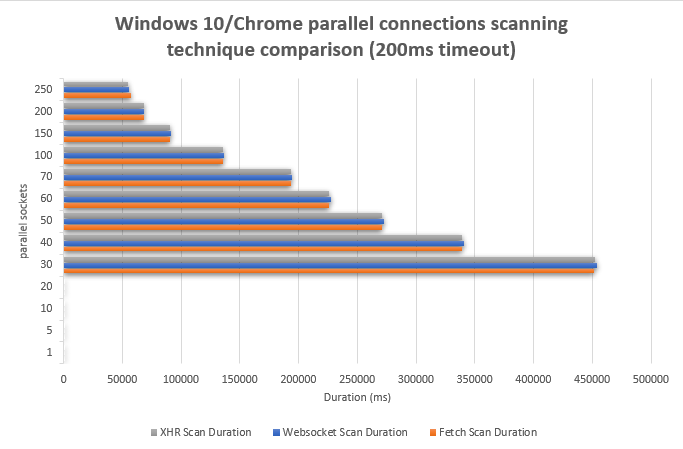
\includegraphics[width=10cm, height=7cm, keepaspectratio]{port_scanning_techniques/img/windows_chrome_scan_technique_comparison.png}
    \caption{Windows/Chrome Parallel sockets efficiency comparison}
    \label{fig:windows_chrome_n_sockets}
\end{minipage}
\hspace{2.6cm}
\begin{minipage}{.45\textwidth}
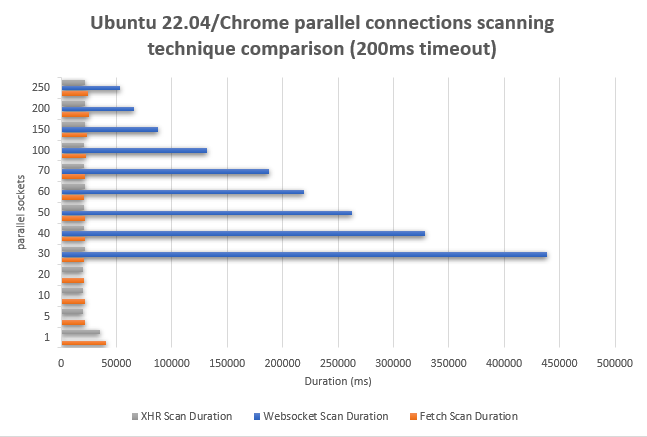
\includegraphics[width=10cm, height=7cm, keepaspectratio]{port_scanning_techniques/img/ubuntu_chrome_scan_technique_comparison.png}
    \caption{Ubuntu/Chrome Parallel sockets efficiency comparison}
    \label{fig:ubuntu_chrome_n_sockets}
\end{minipage}
\end{adjustwidth}
\end{figure}


\subsection{Analysis}

\begin{itemize}

\item \textbf{Optimal number of parallel connections:} We estimate the optimal number of parallel connections to be roughly 10 on Ubuntu, and as high as possible on Windows (250 during our testing). This distinction stems from the fact that Ubuntu does not respect the configured socket timeout, as described in Section~\ref{section:socket-timeout-comparison}. Windows does respect this timeout setting, and is therefore more efficient the more connections it can use. However, when increasing the number of parallel connections on Ubuntu, the socket timeout slowly increases, making the usage of more concurrent connections less efficient. For that reason, it is vital to strike a balance on Ubuntu, which we found to be roughly 10 concurrent connections. 
\item \textbf{Practical Considerations:} Using an excessively high number of parallel connections may seem beneficial in theory (i.e. 200+ parallel connections on Windows) but introduces severe delays and renders the webpage unusable for the user. This practical consideration underscores the irrelevance of establishing a theoretical limit for parallel connections in real-world scenarios.

\end{itemize}

\subsubsection{Conclusion}

The motivation behind this experiment was twofold. Firstly, we aimed to optimize the efficiency of port scanning, focusing on the impact of varying the number of parallel connections when scanning the entire port range (0-65536). Secondly, we sought to identify the potential of a real-world attack by measuring scanning efficiency, providing insights into the feasibility of such attacks.

The experiments have yielded the following findings:

\begin{itemize}
    \item \textbf{Ubuntu vs. Windows Efficiency}: Notable distinctions were observed between Ubuntu and Windows in terms of scanning efficiency. Ubuntu efficiently scanned the entire port range within 25 seconds, whereas Windows took 50 seconds, even with the highest number of parallel connections (250).

    \item \textbf{Balancing Parallel Connections and Timeouts}: Achieving optimal efficiency in port scanning involves striking a balance between the number of parallel connections and socket timeouts. Ubuntu's expedited socket timeouts were closely related to the number of parallel connections, with the most efficient setting observed at approximately 10 parallel connections.

    \item \textbf{Practicality in Real-World Attacks}: Although using a high number of parallel connections may seem theoretically advantageous, it introduces significant delays and renders webpages unusable for users. Therefore, establishing a theoretical limit for parallel connections, such as increasing the count to 256 instead of 250, was deemed irrelevant. In practice, both amounts are impractical for real-world port scan attacks on Windows.

\end{itemize}

In conclusion, this experiment has provided valuable insights into optimizing the efficiency of port scanning techniques. It has demonstrated that the efficiency of port scanning varies significantly between Ubuntu and Windows, with Ubuntu showcasing faster scan times due to its disregard for socket timeouts. The findings emphasize the importance of balancing parallel connections and timeouts to achieve optimal scanning efficiency. Moreover, it highlights the practicality of using browser-based port scanning in practice.



%%%%%%%%%%%%%%
% The second experiment was focused on finding the most effective scanning technique, by comparing the Fetch, XHR and WebSocket APIs. We determine effectiveness by the number of open ports accurately detected. 

% The third experiment focuses on efficiency. The different scanning techniques were used to scan the entire port range (0-65536) using different amounts of parallel connections. While it may seem logical that the highest possible number of parallel connections will result in the most efficient scan, this is not necessarily the case. 

% In order to conduct these experiments, several ports were artificially opened on each system, representing various attack objectives. These attack objectives are TCP ports hosting HTTP servers. 





%% \end{tabular}
%% \caption{Experiment parameters}
%% \end{figure}

% Narayan and Shmatikov~\cite{narayanan201233} found that 33 bits of entropy is enough information to uniquely identify a person. 

% \subsection{Experiment setup}

% Throughout all the experiments, data was systematically gathered with a focus on two key metrics: efficacy and efficiency. Efficacy, in this context, is defined by the count of accurately identified open ports. Efficiency is evaluated by analyzing the speed of the scanning process while ensuring that the efficacy of port detection remains uncompromised.

% The following metrics were collected for each scan:
% \begin{itemize}    % \itemsep-2em 
%     \item A timestamp when the scan started and ended.
%     \item The port number and its status (open/closed)
%     \item Start and end time of each \emph{individual} port scanned
% \end{itemize}

% A port status may also be determined via post-scan analysis through measuring timings, this will be made clear in the results.

% In order to ensure the reproducibility of the experiment, a fully automated approach was implemented using Docker containers. This allows us to encapsulate the entire experiment and maintain consistency throughout. Moreover, we can easily run multiple experiments in a scripted manner, ensuring accurate results.

% The key advantage of utilizing Docker containers is that they provide a self-contained environment, eliminating any potential issues associated with variations in the underlying systems. By specifying parameters through the Dockerfile, we can introduce variations such as operating systems, browsers, socket settings, and scanning techniques while maintaining overall consistency.

% By employing Docker containers for our experiment, we effectively address the challenges related to reproducibility in scientific research. The encapsulation and isolation provided by Docker ensure a consistent experiment environment, regardless of the host system. This, coupled with the ability to concurrently execute numerous experiments with parameter variations, significantly enhances the efficiency and reliability of our research. The setup is depicted in Figure~\ref{fig:experiment}, the parameters for the experiments are listed in Appendix~\ref{appendix:expirement-parameters}


% \clearpage

% \subsection{Results}

% This section presents the outcomes of the conducted experiments aimed at evaluating the effectiveness and efficiency of different scanning techniques for detecting open ports. The raw experimental data is provided in Appendix A.

% \subsubsection{Estimating the optimal socket timeout setting}

% We observed that employing a socket timeout of 100 milliseconds resulted in reduced accuracy for Chrome, with fewer than the intended 100 open ports being detected. The accuracy reached 100\% with a timeout setting of 150ms. Similar outcomes were noticed for Firefox, as outlined in Table~\ref{tab:socket-timeout-comparison}. However, upon validating the results outside the virtualized environment in a real-world scenario, Chrome's accuracy remained consistent at 100\% with a 150ms timeout, whereas Firefox's results were inconsistent until a timeout of 400ms was used.

% This discrepancy in results could be attributed to the more efficient execution of the browser in headless mode, as employed in our experiment. Consequently, after validating the results in a real-world context, we suggest that an optimal timeout setting of 150ms be used for Chrome, and 400ms for Firefox. Notably, these settings are less critical for Ubuntu, as the operating system's automatic request timeout mechanism renders the configured socket timeout less influential. It was observed that on Ubuntu, port responses generally occurred within 5--75ms, irrespective of the configured socket timeout setting.

% \subsubsection{Estimating the most effective scanning technique}

% With the aforementioned timeout settings, we proceeded to compare the Fetch, XHR, and WebSocket APIs to determine the most effective scanning technique. Initial analysis of raw results indicated that the Fetch API outperformed both WebSocket and XHR APIs, as summarized in Table~\ref{tab:scan-technique-comparison}. The Fetch API achieved a 100\% open port detection rate, whereas the XHR and WebSocket APIs failed to detect any open ports.

% This distinction stems from the exclusive capability of the Fetch API to operate in the \emph{no-cors} mode within JavaScript. This mode allows the Fetch API to make cross-domain requests (in our case, requests to localhost) without being hindered by CORS restrictions. However, it imposes significant limitations on the API's functionalities, including the removal of headers from the request, restrictions on Content-Type and request method, and most importantly, the inability to access the response body, status, and headers. Nevertheless, the Fetch API retains the ability to determine whether a port is open, even in the no-cors mode.

% However, this does not imply that the XHR and WebSocket APIs are incapable of detecting open ports. Post-scan analysis allowed us to perform a basic timing attack~\cite{Dhem2000}, which enabled a more comprehensive evaluation of their scanning abilities. By comparing response times between closed and open ports, additional open ports could be detected.

% When comparing response times between open and closed ports, we noticed that open ports always respond faster than the configured socket timeout of 200ms. Therefore, ports responding within <200ms could generally be classified as open. However,\emph{unsafe} ports are an exception to the rule. Unsafe ports will respond quickly, but that does not mean that they are open ports. 

% Unsafe or restricted ports refer to a range of TCP/UDP ports that are reserved for system or administrative use and are not meant for normal application traffic. Browsers do not reveal information about these ports, so we cannot determine whether these ports are open or not. Unsafe ports were excluded from the port scans in Table~\ref{tab:scan-technique-comparison} to prevent data pollution.

% Particularly on the Windows operating system, the XHR and WebSocket  detection capabilities were significantly enhanced when utilizing this timing attack method, enabling the XHR API, similar to the Fetch API, to achieve a 100\% open port detection rate. This is depicted in Figures~\ref{fig:win-chrome-xhr} and~\ref{fig:win-firefox-xhr}.

% \begin{figure}[h]
% \centering
% \begin{minipage}{.45\textwidth}
%   \centering
% 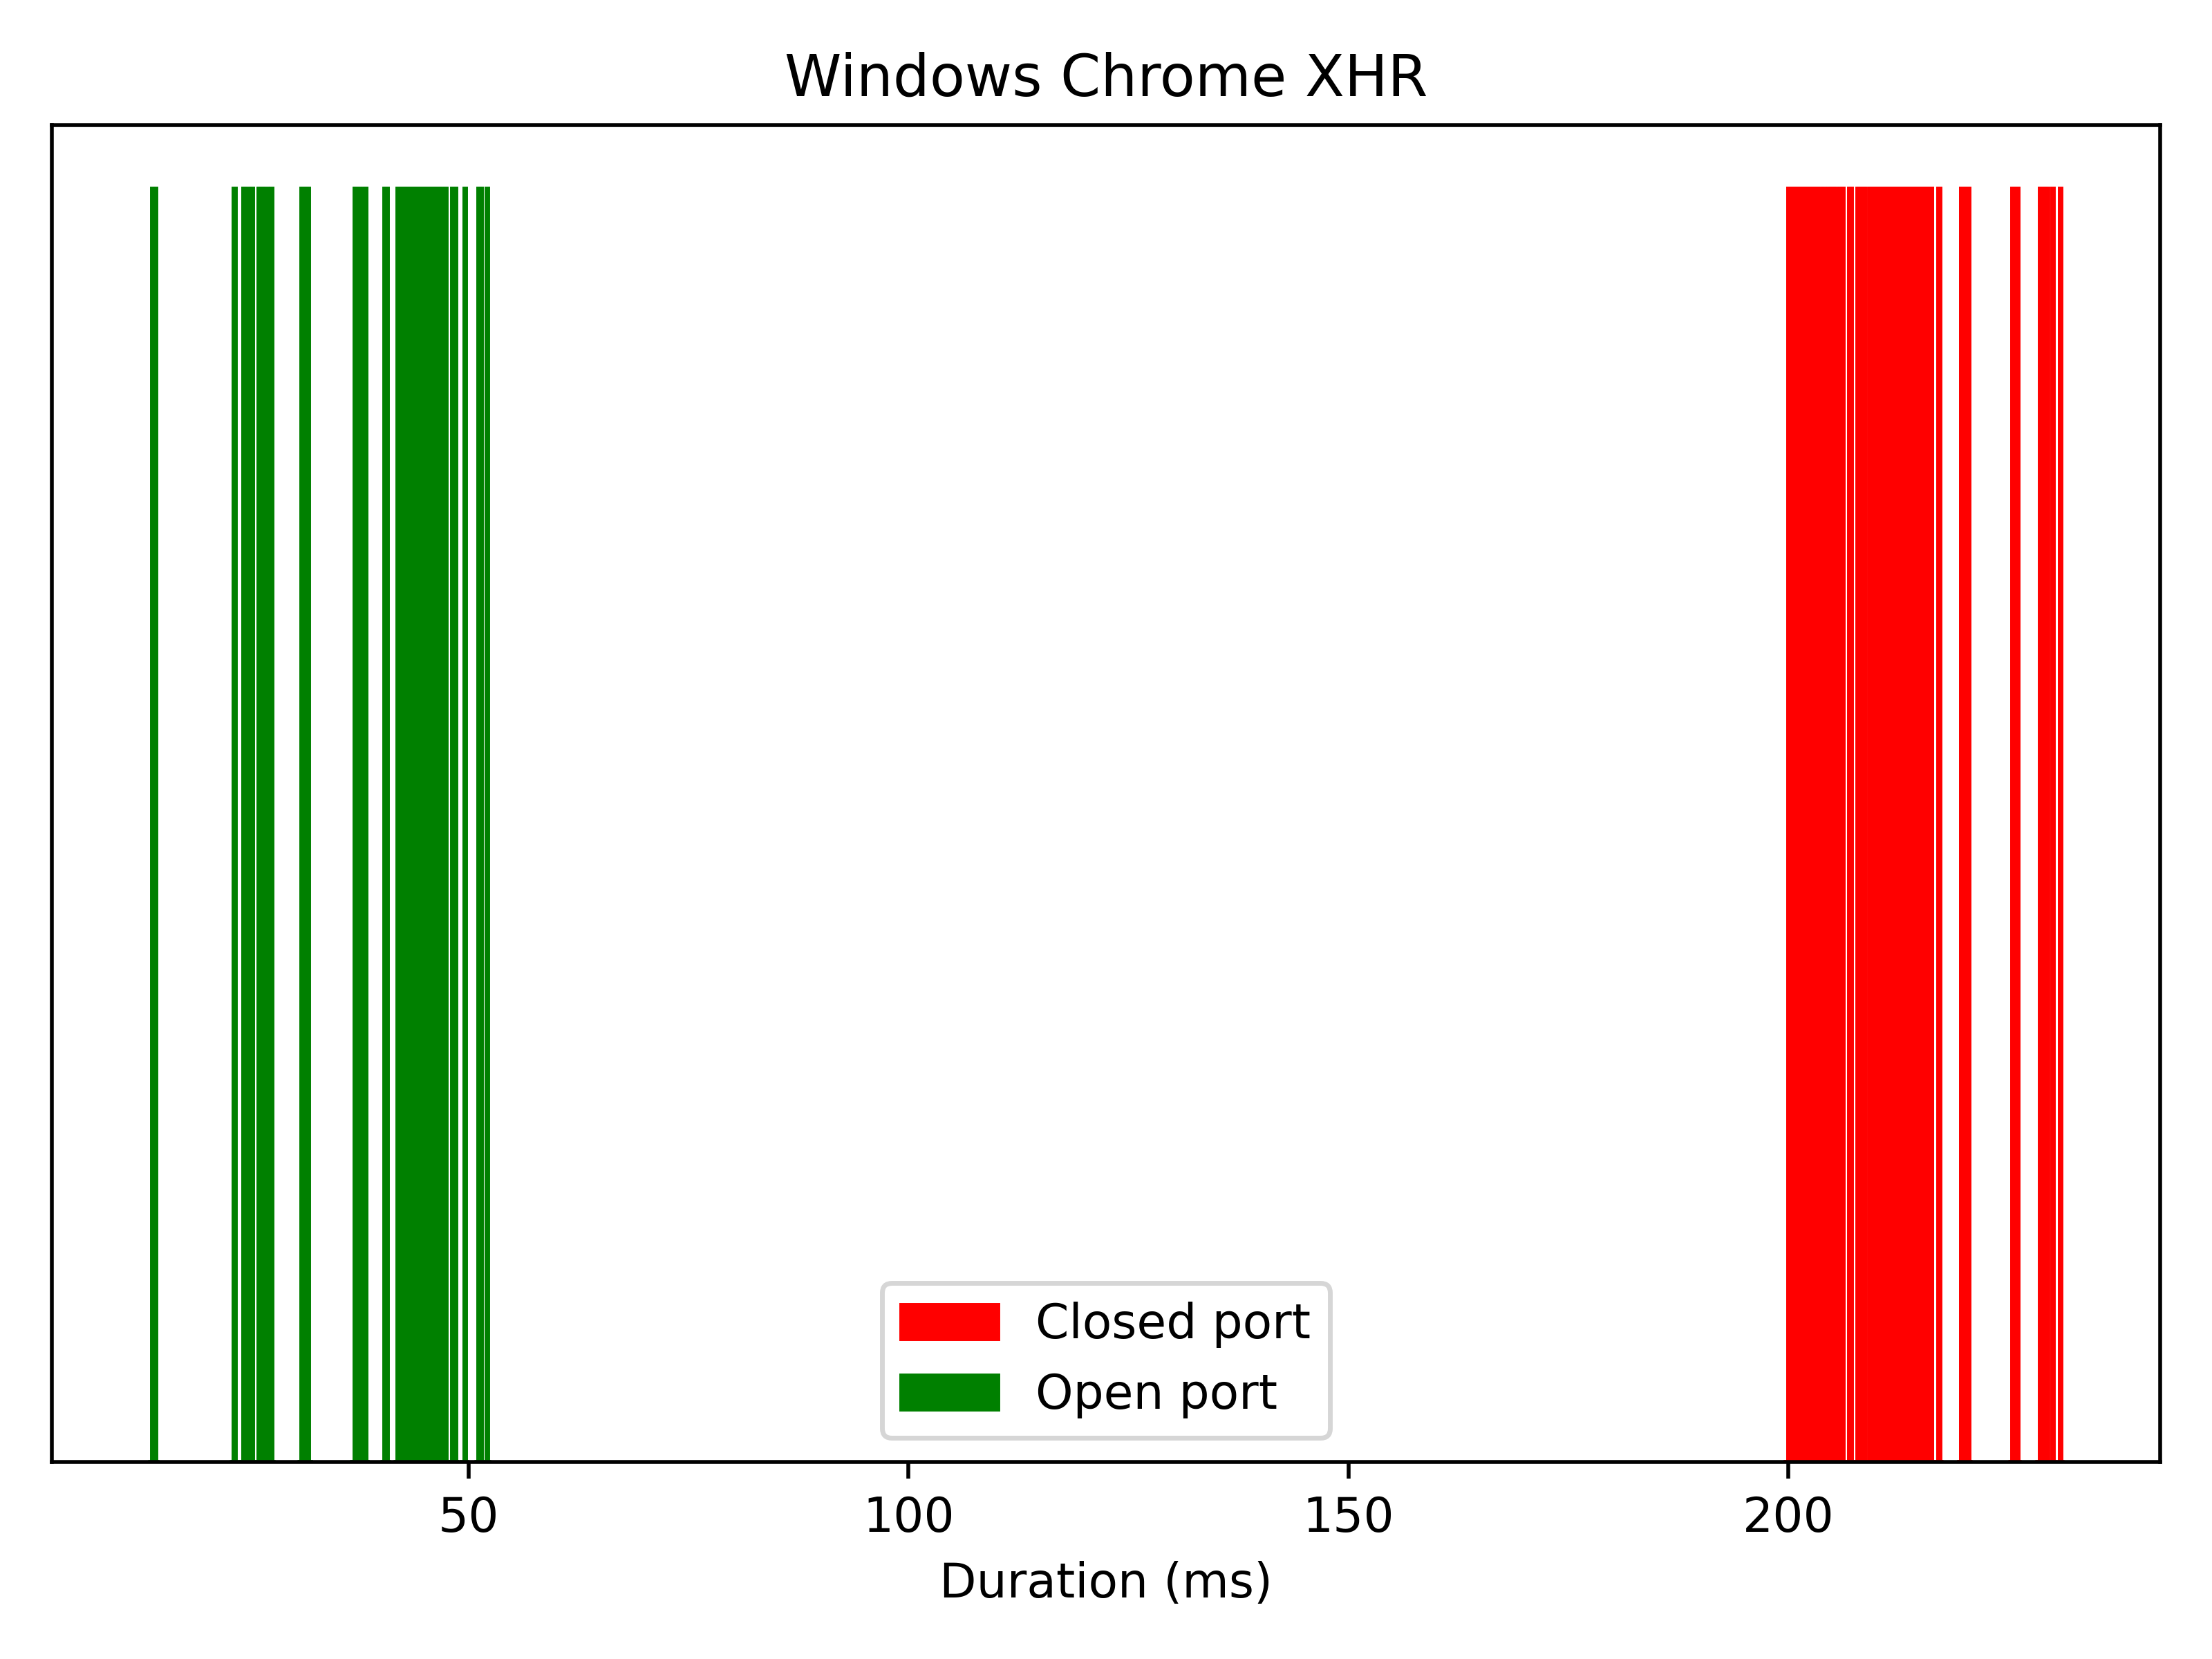
\includegraphics[width=10cm, height=5cm, keepaspectratio]{port_scanning_techniques/img/windows_chrome_efficacy_xhr.png}
%     \caption{Windows/Chrome XHR API scan duration open vs closed ports}
%     \label{fig:win-chrome-xhr}
% \end{minipage}
% \hspace{0.5cm} % Adjust the horizontal space between the two figures
% \begin{minipage}{.45\textwidth}
% \includegraphics[width=10cm, height=5cm, keepaspectratio]{port_scanning_techniques/img/windows_firefox_efficacy_xhr.png}
%     \caption{Windows/Firefox XHR API scan duration open vs closed ports}
%     \label{fig:win-firefox-xhr}
% \end{minipage}
% \end{figure}

% The combination of WebSocket/Firefox also had an increased detection rate of 100\%, but WebSocket/Chrome remained unable to detect any of the open ports, this is depicted in Figures~\ref{fig:win-firefox-websocket} and~\ref{fig:win-chrome-websocket}.

% \begin{figure}[ht]
% \centering
% \begin{minipage}{.45\textwidth}
%   \centering
% \includegraphics[width=8cm, height=4cm, keepaspectratio]{port_scanning_techniques/img/windows_Firefox_efficacy_websocket.png}
%     \caption{Windows/Firefox WebSocket API scan duration open vs closed ports}
%     \label{fig:win-firefox-websocket}
% \end{minipage}
% \hspace{0.5cm} % Adjust the horizontal space between the two figures
% \begin{minipage}{.45\textwidth}
%   \centering
% 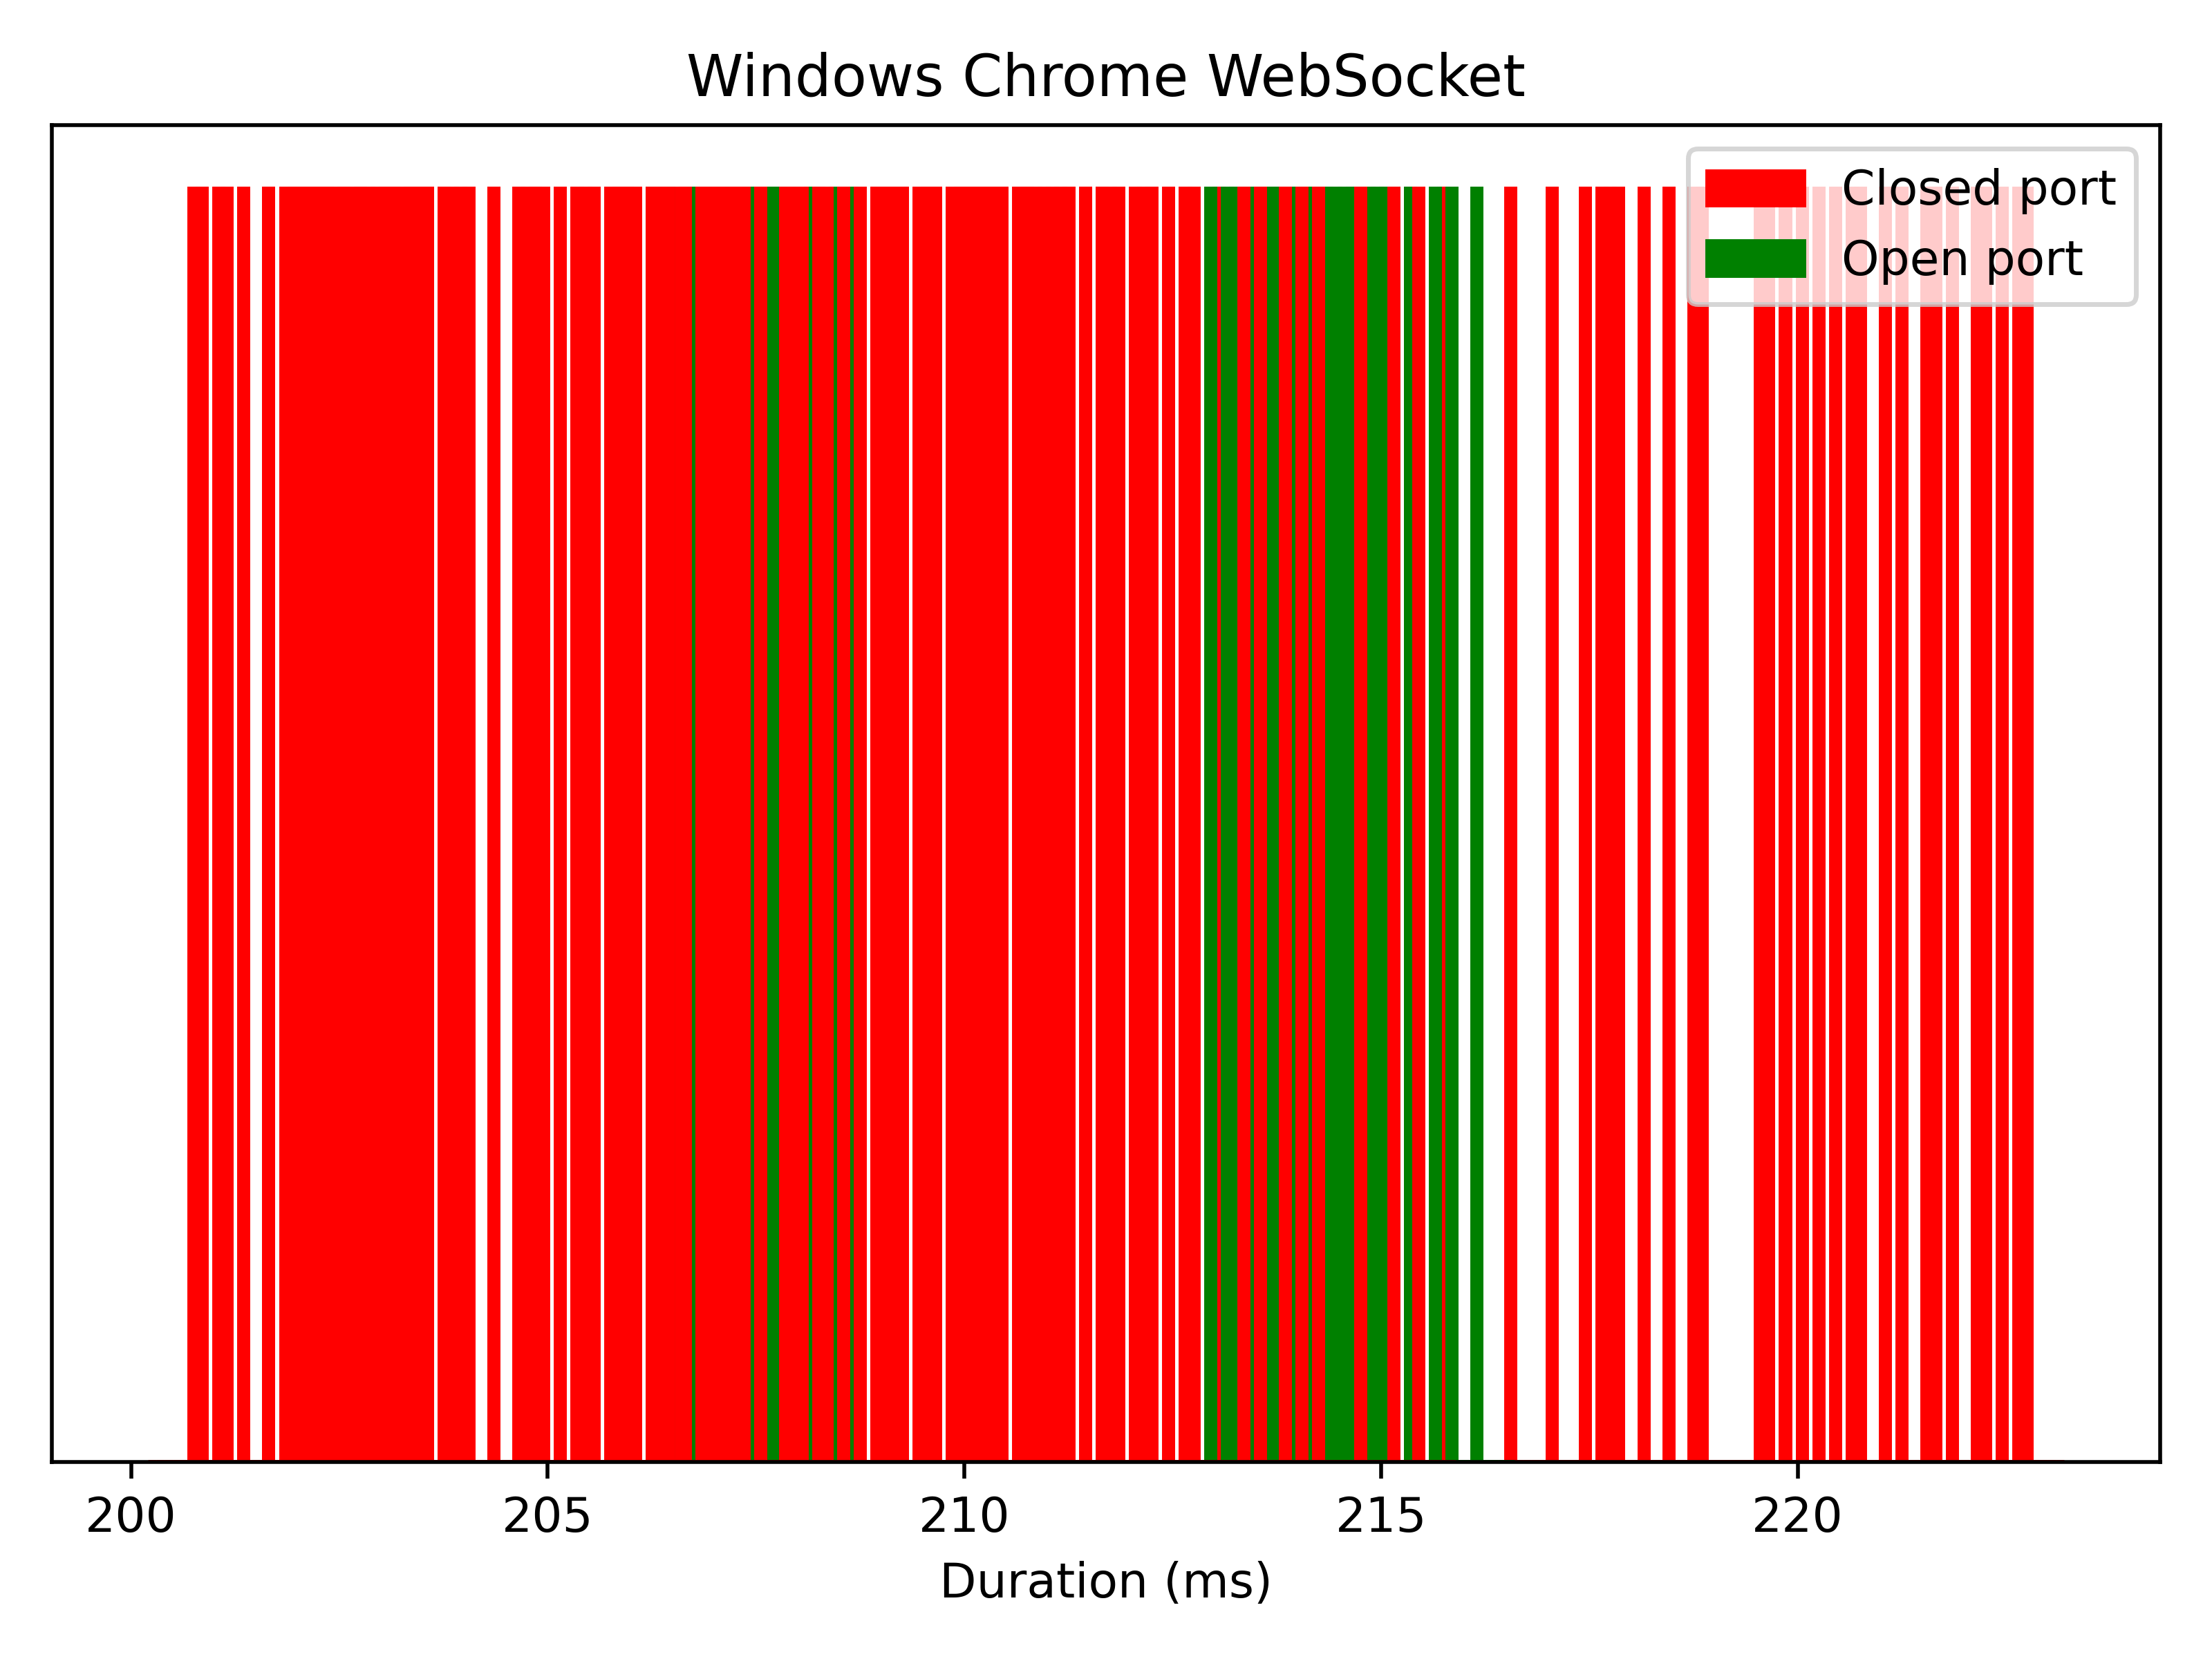
\includegraphics[width=8cm, height=4cm, keepaspectratio]{port_scanning_techniques/img/windows_chrome_efficacy_websocket.png}
%     \caption{Windows/Chrome WebSocket API scan duration open vs closed ports}
%     \label{fig:win-chrome-websocket}
% \end{minipage}
% \end{figure}

% On the contrary, this timing attack method is not useable on the Ubuntu operating system, as there is no clear difference in response times between open and closed ports.

% \subsubsection{Estimating the most efficient scanning technique}

% In this experiment, a comparative analysis of various scanning techniques was conducted to assess their efficiency in scanning the complete port range (0-65536) using different levels of parallel connections. Notable distinctions between Ubuntu and Windows emerged during the utilization of Fetch and XHR APIs, as evidenced in Figures~\ref{fig:windows_chrome_n_sockets} and~\ref{fig:ubuntu_chrome_n_sockets}.

% In the case of Ubuntu, increasing the number of parallel connections does not provide a significant benefit. As soon as roughly 10 parallel connections are used, not much performance gain can be seen when the number of parallel sockets is increased. In fact, performance is slightly decreased with a larger number of parallel connections. 

% Conversely, Ubuntu showed superior performance in scanning individual ports compared to Windows. This discrepancy can be attributed to Ubuntu's disregard for the configured socket timeout of 200ms, a behavior that persisted unless  WebSockets were used. Specifically, under WebSockets usage, Ubuntu's behavior aligned with that of Windows. As a result, the execution of Fetch and XHR connections on Ubuntu occurred notably faster, typically ranging between 5-75ms, in contrast to adhering strictly to the specified 200ms timeout.

% The observed shorter connection timeouts are intrinsically linked to the degree of parallel connections configured. A higher number of parallel connections correlates with an extended timeout duration. Thus, attaining an optimal balance between parallel connections and timeouts proves to be crucial. In this experimental context, the configuration of around 10 parallel connections demonstrated the highest efficiency.

% In conclusion, XHR and Fetch are similar in performance on both Windows and Ubuntu. However, scans complete much faster on Ubuntu than Windows, due to the configured socket timeout not being respected on Ubuntu. WebSockets are similar in performance to XHR and Fetch on Windows, but are significantly outperformed on Ubuntu.  

% \begin{figure}[h]
% \begin{adjustwidth}{-3cm}{-1cm}
% \centering
% \begin{minipage}{.45\textwidth}
%   \centering
% 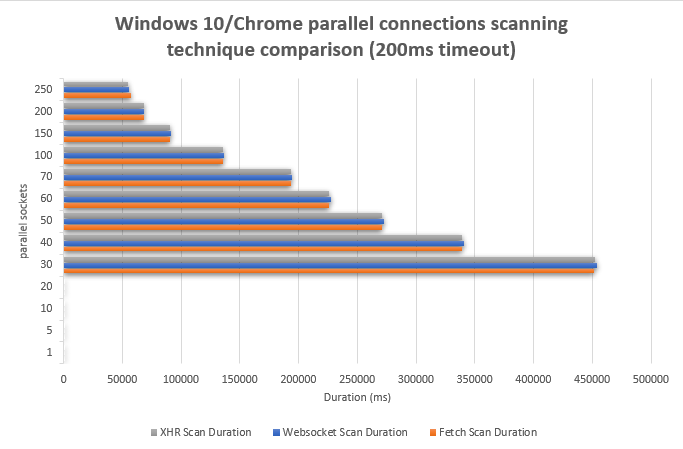
\includegraphics[width=12cm, height=7cm, keepaspectratio]{port_scanning_techniques/img/windows_chrome_scan_technique_comparison.png}
%     \caption{Windows/Chrome Parallel sockets efficiency comparison}
%     \label{fig:windows_chrome_n_sockets}
% \end{minipage}
% \hspace{0.5cm}
% \begin{minipage}{.45\textwidth}
% 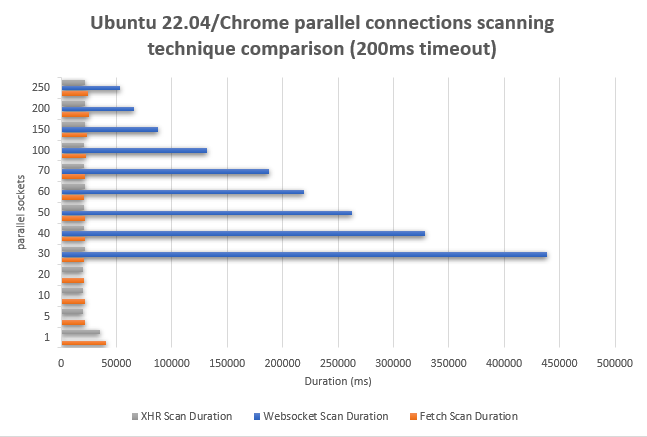
\includegraphics[width=12cm, height=7cm, keepaspectratio]{port_scanning_techniques/img/ubuntu_chrome_scan_technique_comparison.png}
%     \caption{Ubuntu/Chrome Parallel sockets efficiency comparison}
%     \label{fig:ubuntu_chrome_n_sockets}
% \end{minipage}
% \end{adjustwidth}
% \end{figure}


% This optimization on Ubuntu, wherein it disregards the configured socket timeout setting, results in notably faster scans when compared to Windows. 
% Ubuntu completes scanning the entire port range (0-65536) within 25 seconds, whereas Windows takes 50 seconds even with the highest number of parallel connections (250).

% Although using such a high number of parallel connections may seem beneficial in theory, it introduces severe delays and renders the webpage unusable for the user. This consideration underscores the irrelevance of establishing a theoretical limited for parallel connections, such as increasing the count to 256 instead of 250. Both amounts are impractical in real-world scenarios, and a local port scan attack on Windows will not come close to reaching the theoretical limit in practice.




% However, this does not necessarily mean that XHR and WebSockets can not detect open ports. Through post-scan analysis, we can conduct a trivial timing attack~\cite{Dhem2000}, by comparing the response times of the APIs, and comparing the results between open and closed ports. With this methodology, the XHR API can also detect 100\% of open ports, on Windows. 



% \clearpage
% \section{Analysis}

% \subsection{Efficiency}

% There is a clear distinction between Ubuntu and Windows when it comes to running the Fetch and XHR APIs, as can be seen in Figures~\ref{fig:ubuntu_chrome_n_sockets} and~\ref{fig:windows_chrome_n_sockets}. In the case of Ubuntu, increasing the number of parallel connections does not provide a significant benefit. As soon as roughly 10 parallel connections are used, not much performance gain can be seen when the number of parallel sockets is increased. In fact, performance is slightly decreased with a larger number of parallel connections. However, when it comes to scanning individual ports, Ubuntu significantly outperforms Windows. This can be attributed to the fact that Ubuntu ignores the configured socket timeout of 200ms, unless WebSockets are used. In the case of WebSockets, we observe similar behavior to Windows. As a result, Fetch and XHR connections are timed out much faster on Ubuntu, typically within 1-50ms as opposed to the configured 200ms timeout. These timeouts are closely related to the amount of parallel connections. When the number of connections increase, so does the timeout. Striking a balance between parallel connections and timeouts is therefore very important, with the most efficient setting being around 10 parallel connections during our testing. 

% This optimization on Ubuntu leads to significantly faster scans compared to Windows. In just 25 seconds, Ubuntu can scan the entire port range (0-65536), whereas Windows takes 50 seconds even with the highest number of parallel connections (250). Although using such a high number of parallel connections may seem beneficial in theory, it introduces severe delays and renders the webpage unusable for the user. Due to this, determining the theoretical limit for parallel connections, such as 256 connections instead of 250, was considered irrelevant. Both amounts are impractical in real-world scenarios, and a local port scan attack on Windows will not come close to reaching the theoretical limit in practice.

% \subsection{Efficacy}

% As can be seen in appendix A, table~\ref{tab:scan-technique-comparison}, the Fetch API is able to detect 100\% of the open HTTP ports on both Windows and Ubuntu, via the intended functionality of the API. On top of that, both the Fetch and XHR APIs seem to outperform Websockets on both Windows and Ubuntu.

% While it may seem that the XHR API cannot detect any of the open ports, this is not necessarily true. Via post-scan analysis, it is possible to detect the open ports by comparing response times. Open ports respond faster than the configured socket timeout (200ms). Therefore, ports may \emph{generally} be considered open ports when they respond in <200ms. However, \emph{unsafe} ports will respond quickly, but that does not mean that they are open ports. Unsafe or restricted ports refer to a range of TCP/UDP ports that are reserved for system or administrative use and are not meant for normal application traffic. Browsers do not reveal information about these ports, so we cannot determine whether these ports are open or not. Unsafe ports were excluded from the port scans in table~\ref{tab:scan-technique-comparison} to prevent data pollution.

% As can be seen in Figures~\ref{fig:win-chrome-fetch},~\ref{fig:win-chrome-xhr} and~\ref{fig:win-chrome-websocket}, both the XHR and Fetch APIs are able to detect 100\% of open ports through post-scan analysis on Windows. The response times of open ports are significantly faster than closed ports. However, Websockets do not respond faster to open HTTP ports, and can therefore not detect open HTTP ports. As noted before, the configured socket timeout for the scans does not seem to be respected by Ubuntu, this is reflected in figures~\ref{fig:ubuntu-chrome-fetch} and~\ref{fig:ubuntu-chrome-xhr}. Therefore, we cannot rely on response time measurements on Ubuntu. This leaves only the Fetch API as a viable port scanning technique for HTTP webservers on Ubuntu, as opposed to both the Fetch and XHR API on Windows.

% Determining the optimal socket timeout setting is relatively simple. The timeout should be as low as possible while maintaining accuracy. We noticed that a socket timeout of less than 140 milliseconds led to a loss of accuracy on Chrome, resulting in the detection of fewer than 100 open ports. Hence, based on our findings, we conclude that the optimal socket timeout setting for Chrome is roughly 150ms. For Firefox this is less efficient, as we saw a loss of accuracy on 390ms, therefore we conclude that the optimal socket timeout for Firefox is roughly 400ms. 

\section{Experiments Conclusions}

The experiments have resulted in the identification of optimal socket configuration settings for browser-based port scanning. Specifically, it is recommended to utilize a socket timeout of 150ms for Chrome and 400ms for Firefox. For Ubuntu, the most effective number of parallel connections is approximately 10, while on Windows, an increased number of parallel connections, up to 250, is advised. However, due to the associated operational impact on webpage usability, a more practical range of 100-150 parallel connections is recommended for real-world attack scenarios, contingent upon the specific webpage characteristics. 

Among the scanning techniques evaluated, the Fetch API emerges as the optimal choice for browser-based port scanning across both Ubuntu and Windows environments, as well as in browsers such as Chrome and Firefox. The Fetch API exhibits comparable performance to XHR and notably surpasses WebSockets in efficiency. A distinct advantage of the Fetch API lies in its capacity to detect the openness of TCP ports running HTTP services directly, eliminating the necessity for post-scan analysis. This capability is attributed to the utilization of the \emph{no-cors} mode.

When using the optimized scanning configuration, notable speed gains are attainable. For instance, the scanning of 1,000 ports can be achieved within one second using Chrome and within three seconds using Firefox. In broader scans, the entire port range (0 - 65,536) necessitates around 70 seconds for completion on Windows and approximately 25 seconds on Ubuntu. This performance differential stems from Ubuntu's expedited socket timeouts, which diverge from the specified timeout value of 150ms.

In practical applications, port scan attacks typically focus on identifying specific, well-known ports, rather than exhaustively scanning the entire port range. In light of this, browser-based port scanning presents a viable attack vector, capable of scanning more than 1,000 ports per second, thus substantiating its practicality for a real-world attack.


% ~\ref{fig:ubuntu-chrome-websocket}


% \subsubsection{Experiment}

% In order to effectively measure and create the most optimal scanning technique depending on the attack goal, an experiment will be conducted as follows:

% \begin{enumerate}
% \item Open the following ports on the system in different states, representing different attack goals:

% \begin{enumerate}[Port]
% \item 10000: TCP port running HTTP
% \item 10001: TCP port running a WebSocket
% \item 10002: UDP port
% \item 10003: UDS (Unix domain socket) port
% \end{enumerate}

% The expectation is that UDS and UDP ports are undetectable, as client-side JavaScript can only connect to TCP ports. While WebRTC can communicate over UDP sockets, we cannot use WebRTC for port scanning.

% \item Run the port scanner application \cite{bvdl2023} multiple times, using the following steps:
% \begin{itemize}
% \item Enumerate the entire port range (0-65536) using every implemented scanning technique.
% \item Enumerate ports 10000-10003 using every implemented scanning technique.
% \item Rerun the scan by increasing the number of parallel sockets and using the lowest socket timeout possible to achieve the most efficient scanning technique.
% \end{itemize}

% \item Collect the following data for analysis:
% \begin{itemize}
% \item Response time measurements
% \item Identified open ports
% \item Accuracy of the scan results
% \end{itemize}

% This experiment will be conducted on various combinations of browsers and operating systems to determine the most effective scanning technique for each browser/OS.
% \end{enumerate}

\chapter{Fingerprinting Applications}

In this chapter, we focus on the capabilities of browser-based port scanning for identifying programs running locally on a user's system. 

\section{Fingerprinting the underlying operating system}

In this section, we explore the potential of fingerprinting the underlying operating system through browser-based port scanning. As mentioned previously, numerous ports utilized by the operating system fall under the category of unsafe or restricted ports. Consequently, these particular ports remain undetectable through browser-based port scanning.
Nevertheless, certain ports employed by the OS do not carry the restricted classification, allowing us the opportunity to fingerprint and distinguish different OS configurations from each other. 

\subsection{Motivation}

The motivation for fingerprinting the underlying operating system serves a dual purpose, encompassing both privacy and security concerns, each of which carries its own set of implications.

\subsubsection{Privacy Concerns}

Detecting running services on the operating system allows us to distinguish users from each other and potentially track their online activities across multiple browsing sessions. This capability raises significant concerns about user anonymity and invasive tracking practices. Understanding the extent of OS identification and associated privacy risks is crucial to safeguarding user data and online privacy.

\subsubsection{Security Concerns}

Secondly, the ability to detect open ports can have profound security implications. Open ports may represent services or applications running on the system, potentially revealing valuable information to malicious actors. Specifically:

\begin{enumerate}
  \item \textbf{Scanning for known exploits:} Identifying open ports allows for a preliminary assessment of the security posture of an operating system. Some open ports may indicate the presence of services or software that could be vulnerable to known exploits. 
  
  \item \textbf{Attack surface analysis:} Exposed open ports serve as entry points into the operating system, which malicious actors can exploit for various purposes, including unauthorized access and reconnaissance.
\end{enumerate}

\subsection{Experiment Target}
The experiment primarily focuses on identifying running services on both Windows 11 and Ubuntu 22.04 operating systems, using browser-based port scanning. The main objectives are:

\begin{enumerate}
    \item \textbf{Port Scanning:}
    \begin{itemize}
        \item To scan the entire port range on default installations of Windows and Ubuntu.
        \item To identify if there are any open ports that are detectable through browser-based port scanning.
    \end{itemize}

    \item \textbf{Service Activation:}
    \begin{itemize}
        \item To activate various network-related services within the operating systems.
        \item To monitor and record any new ports that become open as a result of these service activations.
        \item To assess the potential for browser-based port scanning to detect these services
    \end{itemize}
\end{enumerate}

\subsection{Experiment Setup}

The experiment was based on default installations of Windows 11 and Ubuntu 22.0.4, with no existing services activated. It involved the following steps:

\subsubsection{Port Scanning}

The browser-based port scanner application as discussed in Section~\ref{section:port-scanner-application} was used to scan the entire port range (0-65536) for both default installations of Windows and Ubuntu.

\subsubsection{Service Activation and Port Monitoring}

To systematically activate network-related services within the operating systems, we followed a manual approach:

\begin{itemize}
    \item On Windows, we methodically enabled every available Windows feature and enabled settings that may require network connectivity, such as Bluetooth, Devices, Phone Link, VPN and Remote Desktop Protocol. After each change, we monitored the status of the ports using the \emph{netstat} command and other command line directives.
    \item On Ubuntu, we adopted a similar process, systematically enabling network-related services and settings, and monitoring if any new ports were opened.
\end{itemize}

\subsubsection{Verification of Port Openings}

Once a port was identified as open after service activation, we conducted two verification steps:

\begin{itemize}
    \item First, we attempted to detect the open port using the port scanner application. 
    \item Second, if the port scanner application did not detect the open port, we verified that the port was not detectable via timing-based attacks.
\end{itemize}

\subsection{Experiment Results}

\subsubsection{Fingerprinting Windows 11}
\label{section:win11-fingerprint}

In our experiment, we conducted a thorough scan across the entire port range on a default Windows 11 installation. Initially, no open ports (beyond the restricted range) were detected. However, after making adjustments to the OS configuration, we successfully identified several open ports. These results are summarized in Table~\ref{tab:windows-features-open-ports}.

\begin{table}[htbp]
\footnotesize
\centering
\begin{tabular}{p{4cm}p{1cm}p{2cm}p{8cm}}
    \toprule
    Windows Feature & Open Port & Associated Process & Description \\
     \midrule
     Hyper-V & 2869, 5357 & svchost.exe, ntoskrnl.exe, vmms.exe & Enabling the Hyper-V Windows feature, which provides a native hypervisor, led to the opening of ports 2869 and 5357. These ports were associated with processes such as svchost.exe, ntoskrnl.exe, and vmms.exe. Hyper-V is commonly used for running virtual machines and containers, making these ports relevant for detection. \\
     
     Internet Information Services (IIS) & 80 & InetMgr.exe, ntoskrnl.exe & Enabling Internet Information Services (IIS) resulted in port 80 becoming open, as it hosts a default website. The process responsible for this port was ntoskrnl.exe, which is integral to the Windows operating system. \\
     
     Microsoft Message Queue (MSMQ) Server & 50921 & mqsvc.exe & While enabling MSMQ temporarily opened port 50921, it falls within the dynamic port range and is not suitable for reliable fingerprinting. \\
     \bottomrule
\end{tabular}
\caption{Windows Features and their associated open ports}
\label{tab:windows-features-open-ports}
\end{table}

Additionally, Windows contains a default mapping of well-known ports in the 

\texttt{\%WINDIR\%\textbackslash System32\textbackslash drivers\textbackslash etc\textbackslash services} file, including approximately 100–135 ports outside the restricted range, which can serve as a foundation for targeted scans.
Aside from Windows features, there are standard settings that may be enabled or disabled on Windows. We tested for open ports (outside the restricted range) on settings that require network connectivity, such as Bluetooth, Devices, Phone Link, VPN and Remote Desktop Protocol.

Among these, VPN and Remote Desktop Protocol (RDP) exhibited noteworthy findings. While a VPN connection might not be detectable by itself, our tests involving ExpressVPN revealed an interesting aspect. The ExpressVPN application seemed to open port 2020, which we could consistently detect while the VPN was active. This implies that although the Windows OS does not inherently trigger the opening of a specific port upon VPN configuration, the VPN application itself does so.
Regarding RDP, establishing a connection to a remote machine does not appear to expose any open ports on the host machine. However, on the machine to which the connection is made, we were able to identify the presence of an active RDP connection. While the Fetch API does not directly identify that the RDP port (3389) is open, we managed to determine that the port was open via a timing attack. This approach enables us to detect the open port consistently. This finding suggests that browser-based port scanning remains a viable method for detecting remote access tools, similar to the technique employed by eBay in 2020~\cite{ebay_port_scans}.

\subsubsection{Fingerprinting Ubuntu 22.04}

In our examination of a default installation of Ubuntu 22.04, we consistently found port 631 to be open. This port corresponds to the Common Unix Printing System (CUPS), a printer software driver.
Besides CUPS, we did not find other services that were detectable through browser-based port scanning after enabling several network-related services, similarly to Windows.
However, like Windows, Ubuntu maintains a \texttt{/etc/services} file, mapping 326 well-known ports to services. While most of these ports fall within the restricted range, approximately 150–180 ports are outside it, providing a basis for fingerprinting different Ubuntu OS configurations.

\subsection{Analysis}

For Windows 11, specific Windows features and network-related settings result in detectable open ports. Enabling features like Hyper-V and Internet Information Services (IIS) resulted in identifiable open ports, making them valuable indicators for distinguishing different Windows configurations. 
In the case of Ubuntu 22.04, the consistent presence of port 631 associated with CUPS simplifies the identification of default Ubuntu installations. 
Simply scanning port 631 will be enough to detect a default Ubuntu installation. While it may not guarantee a 100\% accuracy of the OS fingerprint, another service could be running on port 631, or CUPS could be running on a different OS, its integration with existing techniques improves the reliability of the OS fingerprint. 
The \texttt{/etc/services} file found on both Windows and Ubuntu can be used for a targeted scan on a system, after detecting which OS is making the request. All ports within the \texttt{/etc/services} file can be scanned in one second, making it a realistic enhancement to existing fingerprinting techniques.  

\subsection{Conclusion}

The experiment demonstrated that specific configurations and features in both Windows 11 and Ubuntu 22.04 can lead to identifiable ports on the system.
On Ubuntu, the consistent presence of port 631 associated with CUPS simplifies the identification of default Ubuntu installations, and may strengthen existing fingerprinting techniques related to OS detection.
The experiment also underscored the relevance of timing attacks and browser-based port scanning techniques for detecting open ports, particularly in scenarios such as identifying active RDP connections.

In conclusion, the experiment indicates that by incorporating browser-based port scans into existing fingerprinting techniques, we can significantly enhance their effectiveness. This enhancement not only increases the uniqueness of the fingerprint, but also enables more sophisticated user tracking across browser sessions, which has implications for user privacy.
Furthermore, browser-based port scanning has the capability to identify certain running operating system services. This aspect may be of particular interest to malicious actors seeking to exploit known services operating on specific ports.
Additionally, browser-based port scanning can serve as a defensive measure. It can be employed to block users who are being controlled through remote access tools, a technique previously used by eBay~\cite{ebay_port_scans}.



% \subsection{Fingerprinting Windows 11}
% \label{section:win11-fingerprint}

% When conducting a scan across the entire port range on a default Windows installation, no open ports (beyond the restricted range) were detected. Nevertheless, after making adjustments to the OS configuration, we managed to identify several open ports. On Windows, there are certain features known as \emph{Windows features} that can be enabled or disabled. Enabling some of these Windows features can result in the opening of ports on the system that are detectable. We tested every available Windows feature, the features that opened a port are listed in table~\ref{tab:windows-features-open-ports}

% \begin{table}[htbp]
% \footnotesize
% \centering
% % \begin{adjustwidth}{-1.0cm}{}
% \begin{tabular}{p{4cm}p{1cm}p{2cm}p{8cm}}
%     \toprule
%     Windows Feature & Open port & Process & Description \\
%      \midrule
%      Hyper-V & 2869, 5357 & svchost.exe, ntoskrnl.exe, vmms.exe & The Hyper-V windows feature enables a native hypervisor on the system. Systems running virtual machines, containers or WSL usually have this feature enabled. When this feature is enabled, a process vmms.exe is spawned, which manages Hyper-V. This process, as well as generic system processes on Windows such as svchost.exe and ntoskrnl.exe were found to open ports 2869 and 5357. \\
     
%      Internet Information Services (IIS) & 80 & InetMgr.exe, ntoskrnl.exe & IIS is a popular webserver on Windows which can be enabled through windows features. When enabled, the webserver hosts a default website on port 80. Similarly to Hyper-V, the system process ntoskrnl.exe is responsible for the open port. \\

%      Microsoft Message Queue (MSMQ) Server & 50921 & mqsvc.exe & MSMQ is another windows feature that can be enabled. During our testing, it temporarily opened port 50921, however, this is an ephemeral port in the dynamic port range. Therefore, we cannot use this port for fingerprinting purposes. \\
%      \bottomrule
% \end{tabular}
% % \end{adjustwidth}{}
% \caption{Windows features open ports}
% \label{tab:windows-features-open-ports}
% \end{table}

% \clearpage

% Aside from Windows features, there are standard settings that may be enabled or disabled on Windows. We tested for open ports (outside the restricted range) on settings that require network connectivity, such as Bluetooth, Devices, Phone Link, VPN and Remote Desktop Protocol. These are all settings that are natively supported by Windows, and we therefore consider them to be OS configurations. 

% Among these, VPN and Remote Desktop Protocol (RDP) exhibited noteworthy findings. While a VPN connection might not be detectable by itself, our tests involving ExpressVPN revealed an interesting aspect. The ExpressVPN application seemed to open port 2020, which we could consistently detect while the VPN was active. This implies that although the Windows OS does not inherently trigger the opening of a specific port upon VPN configuration, the VPN application itself does so.

% Regarding Remote Desktop Protocol (RDP), establishing a connection to a remote machine does not appear to expose any open ports on the host machine. However, on the machine to which the connection is made, we were able to identify the presence of an active RDP connection. While the Fetch API does not directly identify that the RDP port (3389) is open, we managed to determine that the port was open via a timing attack. This approach enables us to detect the open port consistently. This finding suggests that browser-based port scanning remains a viable method for detecting remote access tools, similar to the technique employed by eBay in 2020~\cite{ebay_port_scans}.

% Apart from these settings, Windows contains a default mapping of well-known ports in the \texttt{\%WINDIR\%\textbackslash System32\textbackslash drivers\textbackslash etc\textbackslash services}. file. This document includes mappings for 278 ports linked to common system processes and programs. The majority fall within the restricted range, preventing detection, but approximately 100-135 ports are outside this range, serving as a foundation for targeted scans on a system.

% \subsection{Fingerprinting Ubuntu 22.04}

% In a default installation of Ubuntu 22.04, port 631 consistently appeared open. This port corresponds to CUPS, a printer software driver. Contrary to Windows, identifying a default Ubuntu installation becomes relatively straightforward by scanning for this open port. While relying solely on this does not ensure a 100\% accuracy in OS fingerprinting, its integration with existing techniques does improve the reliability of the fingerprinting process.

% Beyond CUPS, adjustments were made to various OS settings requiring network connectivity, mirroring the process on Windows. No opened ports were discovered. Nevertheless, similarly to Windows, Linux features an \texttt{/etc/services} file, mapping 326 well-known ports to services. While most fall within the restricted range, around 150-180 ports are outside it. This presents a solid basis for fingerprinting different Linux OS configurations.

\section{Identifying running programs}

To establish the potential for fingerprinting applications via browser-based port scanning, we selected a limited number of applications from various categories and performed browser-based port scanning to confirm their detectability. The categories target different type of applications to establish the potential of user-profiling.

\subsection{Motivation}

The motivation behind identifying running programs bears a resemblance to the process of fingerprinting the underlying operating system. This similarity extends to encompass concerns related to privacy and security.

\subsubsection{Privacy Concerns}

Detecting running programs gives websites the potential to learn about personal information of users. This can be achieved by mapping common programs to their default ports, and scanning for these ports using browser-based port scanning. Consequently, this capability can be used to identify the individual preferences of users, such as their preferred software applications. This data can be used for various purposes, including crafting personalized advertisements, as well as potentially more nefarious applications like phishing.
Moreover, akin to the practice of OS fingerprinting, the identification of open ports can be utilized to generate a unique fingerprint, enabling the tracking of users across multiple browsing sessions. This persistent tracking can lead to a loss of anonymity and privacy, as users' online behaviors become more traceable.

\subsubsection{Security Concerns}

Secondly, the capacity to detect open ports holds security implications. Much like OS fingerprinting, the identification of running programs may be exploited to target known vulnerabilities within those programs. 

\subsection{Experiment Target}

The experiment focuses on identifying running programs in order to assess the feasibility of browser-based port scanning. We have chosen a select few categories to concentrate on, with the aim of targeting various types of programs and users.
These categories can be broadly categorized into three main groups: user privacy, user preferences, and fingerprinting. Within these main categories, we have chosen a limited number of subcategories to specifically target different types of programs.

\begin{enumerate}
    \item \textbf{User privacy:}
    \begin{itemize}
        \item Video / Chat
        \item VPN
    \end{itemize}
    \item \textbf{User preferences:}
    \begin{itemize}
        \item Entertainment
        \item Gaming
        \item Programming
    \end{itemize}
    \item \textbf{Fingerprinting:}
    \begin{itemize}
        \item Operating System
        \item Web Browser
        \item Peripherals
        \item Automation framework
    \end{itemize}
\end{enumerate}

\subsection{Experiment Setup}

The setup for the experiment is similar to fingerprinting the underlying OS.

\begin{enumerate}
    \item \textbf{Launching the Programs}: For each target program, a repeatable verification process was carried out. This process involved launching the application and using PowerShell directives, namely \texttt{Get-NetUDPEndpoint} and \texttt{Get-NetTCPConnection}, to determine if the application had opened any local ports.
    
    \item \textbf{Verifying Detectable Ports}: The browser-based port scanner application as discussed in Section~\ref{section:port-scanner-application} was used to verify if any of the newly opened ports were detectable. Additionally, response times were measured for post-scan analysis.   

    \item \textbf{Verifying Detectability Through Timing Attacks}: Response times were compared to closed ports, in order to verify whether ports were detectable through timing measurements.
\end{enumerate}

The experiment was conducted on a testing machine using Windows 11 and Chrome 114. 

\subsection{Experiment Results}

The results of the scanned applications are presented in Table~\ref{tab:identifying-applications}.

\begin{table}[htbp]
\footnotesize
\centering
\begin{adjustwidth}{-0.5cm}{}
\begin{tabular}{p{2cm}p{2cm}p{1cm}p{1cm}p{1cm}p{1cm}p{1cm}p{5cm}}
    \toprule
    Category & Application & \multicolumn{2}{c}{opened ports} & \multicolumn{2}{c}{detected ports} & Resp. Time & Notes\\
     \cmidrule{3-4} \cmidrule{5-6} \cmidrule{7-7}
     & & TCP & UDP & TCP & UDP & in ms & \\
     \midrule
     Video / Chat & Discord & 6463 & -- & 6463 & -- & 105,3 & Port 6463 is running HTTP. \\
     Video / Chat & MS Teams & 62391 62390 62389 62388 62368 & 50811 & -- & -- & >200 & No TCP ports in a listening state. \\
     Entertainment & Spotify & 57621 60933 60937--60954 & -- & 57621 60933 & -- & 66.69 39.59 & Many ports in 609xx range with established TCP connections, but only ports 56721 and 60933 in a Listening state. \\ 
     Operating System & Windows Store & 63503 63504 63506 63507 & -- & -- & -- & >200 & No TCP ports in a listening state. \\ 
    Programming & Visual Studio Code & 51736--51763 & -- & -- & -- & >200 & No TCP ports in a listening state. \\ 
    Gaming & Steam & 53245 53237 53236 27060 27036 & -- & 27060 & -- & 120.19 & Many ports in Established state. Only port 27060 in a Listening state. \\ 
    VPN & ExpressVPN & 54719 2020 & -- & 2020 & -- & 56.79 & Ports 2020, 54719 in a listening state. \\ 
    Automation framework & Selenium & 59542. 59536 59536 30454 & -- & 30454 & -- & 72.39 & \\ 
    Web Browser & Edge & 61773--61849 & -- & -- & -- & >200 & No TCP ports in a listening state. \\ 
    Peripherals & Logitech G HUB & 9010 9080 9100 45654 & -- & 9010 9080 9100 45654 & -- & 68 31.1 60.6 62.9 & All ports running HTTP. \\ 
     \bottomrule
\end{tabular}
\end{adjustwidth}{}
\caption{Identified open ports on a testing machine using Windows 11 and Chrome 114}
\label{tab:identifying-applications}
\end{table}
\clearpage

\subsection{Analysis}

We drew several conclusions from these results. In general, TCP ports running HTTP were reliably detectable, as HTTP servers will return an HTTP response code regardless of whether the request succeeded or not. We see many examples of this in the results, such as the Discord, Selenium, and Logitech G HUB applications. Furthermore, scanning for open HTTP ports can be done quickly, because HTTP servers respond quickly, making this fingerprinting technique a realistic attack vector. Additionally, since HTTP ports can be detected by examining the error code in the response, there is no need to measure response times.

Detecting TCP ports that do not run HTTP is more challenging, because they do not respond with HTTP status codes, making them less easily detectable. However, we found that some open TCP ports not running HTTP, such as Spotify and ExpressVPN, have response times that differ significantly from the configured socket timeout of 200ms. In contrast, closed ports typically time out between 200-215ms. Therefore, when TCP ports respond within less than 200ms, they can usually be considered open ports. This suggests that measuring response times of TCP ports could be a reliable fingerprinting technique, but it has some limitations.

Response times depend on several factors, such as the operating system, browser, underlying hardware, and network configuration. Moreover, as previously mentioned, \emph{unsafe} ports will respond quickly, but that does not mean that they are open ports. Additionally, as found in Section~\ref{section:socket-timeout-setting}, this method of using timing attacks will not work on Ubuntu, because the socket timeout of 200ms is not respected like it is on Windows. 
For this reason, we conclude that applications that open a TCP port outside the restricted/unsafe range running HTTP(S) are reliably detectable using the Fetch API. TCP ports not running HTTP can sometimes be detected using timing attacks, depending on the platform. We saw similar behavior in Section~\ref{section:win11-fingerprint}, where an RDP connection was not directly detected by the Fetch API, but was still detectable via a timing attack.

\subsubsection{Mapping applications to open ports}

Having successfully demonstrated the feasibility of reliably fingerprinting certain applications through browser-based port scanning, the next logical step would involve establishing a correlation between applications and the associated open ports. This correlation would significantly enhance our fingerprinting capabilities. However, this task leans more towards an engineering problem rather than a research problem. As a result, we did not emphasize the development of this mapping in our current work.
Nonetheless, it is worth noting that there are existing mappings available that can serve as a solid foundation for fingerprinting purposes, even if they are not exhaustive. Among these mappings, the one hosted by the Internet Assigned Numbers Authority stands out as the most extensive dataset currently available~\citetechnical{iana_ports}. This dataset maps over 10,000 ports to known applications and services.

\subsection{Conclusion}

The detection of open ports using browser-based port scanning, particularly those running HTTP services, proves to be a feasible and reliable, showcasing the potential for this approach as a fingerprinting technique. 
Motivated by privacy and security concerns, the ability to identify running programs has important implications. Privacy concerns arise from the potential for websites to collect information about users' running programs, potentially leading to personalized targeting and tracking across browsing sessions. On the security front, the identification of open ports can serve as an entry point for malicious attackers to gather information and target vulnerabilities within these programs. 

\section{Identifying specific program states}

Beyond determining the mere existence of open ports, the next step involves detecting specific application states. We investigated scenarios where an application's behavior might change its network requirements, leading to the opening of new ports. For instance, when initiating a video call within an application, does it dynamically open new ports to facilitate the communication, and more importantly, can we detect this change through browser-based port scanning? 

\subsubsection{Motivation}

If it becomes possible to detect specific application states, this would elevate user tracking to an advanced level. Websites would gain the capability to determine a user's ongoing activities on their computer, and subsequently, use that information to determine what content to display. This could involve showing different advertisements, presenting webpages tailored to the user's preferences, or, in more concerning scenarios, even creating custom phishing websites based on the user's recent actions.

\subsubsection{Experiment Target}

To investigate this, we selected a limited number of privacy-sensitive applications, and determined if we could detect specific application states, 
such as being able to detect a voice call on Microsoft Teams, or sending/retrieving a text message on WhatsApp.

\textbf{Applications:}
\begin{itemize}
    \item Microsoft Teams
    \item Discord
    \item WhatsApp
    \item Telegram
    \item Chrome
    \item Firefox
\end{itemize}

\subsubsection{Experiment Result}

Across the investigated applications, the same behavior was consistently measured regarding port activity and detectability:

\textbf{Ephemeral Ports:} Applications consistently used ephemeral ports from the dynamic port range (49152-65535) for various activities, such as sending chat messages, initiating video calls, sharing files, collaborating on a document, and initiating file downloads. These ports were short-lived and changed with each instance, making it impossible to establish a direct connection between open ports and specific application states.

\textbf{Port Detectability:} Despite the consistent use of ephemeral ports, these ports were undetectable through browser-based port scanning techniques. This lack of detectability is primarily due to the ports being in an established connection state, which means they were not actively listening for new connections. Consequently, attempts to identify these ports through browser-based port scanning proved ineffective.

\subsubsection{Identifying mobile apps}

While our research is not primarily focused on mobile applications, we conducted preliminary research to assess the viability of using browser-based port scanning to detect mobile applications. In an experiment, we evaluated 70 mobile apps on an Android 11 device, but we were unable to detect a single application through browser-based port scanning. 
It is important to note that we do not consider our research to be definitive in concluding that browser-based port scanning is not a threat on mobile devices, as our study was not as comprehensive as it was for desktop applications. We do not see a reason why browser-based port scanning \emph{should} not be possible on mobile. However, it is worth noting that we did not encounter the same challenges when detecting the first application on desktop devices, as it required considerably less time to detect the first application on a desktop device.

% \subsection{Video / Chat service}

% In this category, we have chosen two widely used video and chat services: Microsoft Teams, a popular enterprise-grade software, and Discord, a popular consumer-grade software. Both of these platforms are well-known for their video and chat capabilities.

% These two applications exhibit comparable functionalities: sending chat messages, initiating video calls, and exchanging files. Microsoft Teams has additional native integration with cloud services such as Office 365 applications and cloud storage. All the functionalities mentioned above necessitate network connectivity, and as a result, we have conducted scans to see if we can differentiate these application states using browser-based port scanning.

% During a video call in Microsoft Teams, specific ports such as 55076 and 60449 were opened, but these ports could not be detected through browser-based port scanning. This is because the ports are in an established state, and not listening for new connections. Notably, making changes during the call, such as activating a camera, did not result in the opening of new ports. It is worth noting that even if these ports were detectable, this would not be very effective due to their ephemeral nature; they change with every session. In other words, the next time a video call is initiated, it will not be the same ports (55076 and 60449), but rather random ones within the dynamic port range (49152--65535) that will be opened.

% Sending chat messages did not open any new ports. On the other hand, sharing files through Microsoft Teams did trigger the opening of several ports. Some of these were related to the Microsoft Teams platform, while others pertained to OneDrive, the underlying cloud-based file sharing service. However, similar to what was observed with video calls, all of these ports were short-lived and ephemeral, which means they varied with each instance. 

% Consequently, this setup makes it extremely challenging to employ browser-based port scanning for fingerprinting these specific application states. This is because any application has the capability to utilize a port within the dynamic port range, and it is not possible to establish a direct connection between the open port and the underlying application through browser-based port scanning.

% In the case of Discord, the same behavior was seen as in Microsoft Teams. Ephemeral ports were generated during video calls, and there was no discernible change in state when sending text messages. The only distinction was the absence of OneDrive-related ports opening during file sharing activities.

% \subsection{Messaging Apps}

% This category focuses on alternatives to desktop native communication apps such as Microsoft Teams and Discord. Here, we focus on mobile-first messaging applications through WhatsApp and Telegram. 

% These applications can similarly send chat messages, initiate video calls, and share files. However, we differentiate them as they are mobile-first applications and are therefore designed differently. 

% When sending a text message on these applications, we see the exact same behavior as before. An ephemeral port is opened within the dynamic port range (49152-65535), this port is undetectable through browser-based port scanning and different each time a message is sent. 

% \subsection{Web browser}

% This category focuses on web browsers, an interesting category due to the numerous existing fingerprinting techniques already applied to them. Our investigation within this category centers around determining whether web browsers open new local ports under specific scenarios: accessing a webpage, streaming a video, opening a new tab, and initiating file downloads. The focus is on the Google Chrome and Firefox browsers.

% Our findings reveal that all the aforementioned actions, except for opening a new tab, result in new ports being opened within the dynamic port range. Typically, around 20 to 30 ports are opened. However, it is important to note that these ports are immediately in an established connection state and do not enter a state where they are actively listening for new connections. As a result, these ports remain undetectable through browser-based port scanning. Similar to the patterns observed in other categories, these ports are randomly selected from the dynamic port range and are ephemeral.


% \subsection{Methodology}

% To conduct this research, we followed a methodology similar to our previous approach. We selected a 
% restricted number of applications from various categories and utilized the PowerShell \texttt{Get-NetUDPEndpoint} and \texttt{Get-NetTCPConnection} commands to analyze the local system. Whenever an action was executed within the application, we monitored for any new ports that became active. Subsequently, we used the port scanner application to probe these newly opened ports. This involved either directly utilizing the Fetch API or using timing attacks.

% \subsection{Results}

% Starting with the same with applications that were identified in Table~\ref{tab:identifying-applications}. When joining a voice channel on Discord, several TCP and UDP ports are opened locally on the system. The same behavior is seen when screen sharing. All ports opened are ephemeral and use a different port number every time, mostly within the 50000-65000 range. However, none of these ports were detected using the Fetch API or timing attacks. 

% The Logitech G HUB application, used for Logitech peripherals, was detectable in a different states. When the application is updating, a new process lghub\_updater.exe is launched which opened port 22885. This port was also detectable through browser-based port scanning.

% \chapter{Extending Existing Fingerprinting Methods and Analyzing Entropy}

% In this chapter, our goal is to extend an existing dataset of fingerprints by incorporating browser-based port scanning data and subsequently analyze the resulting changes in entropy. We aim to explore how the addition of browser-based port scanning data enriches our fingerprint dataset and investigate the differences in entropy that emerge as a consequence.

% Our investigation is centered on entropy analysis, a powerful tool for quantifying the level of randomness and diversity within fingerprints. By comparing the entropy of the extended dataset with the original, we seek to uncover whether the integration of port scanning data significantly alters the uniqueness and complexity of the fingerprints.

\chapter{Estimating the Entropy of Browser-Based Port Scanning}

%% \section{Research Objective}

The primary objective of this chapter is to analyze and compare the entropy of synthetic fingerprint datasets under various scenarios. The focus is on understanding how changes in the distribution of open ports and other attributes influence the uniqueness and complexity of fingerprints. 

\subsubsection{Motivation}

The core motivation driving this research is user privacy, particularly user anonymity. As digital fingerprinting techniques continue to advance, the granular details of a user's device, such as the number and identity of open ports, can be key factors in influencing fingerprint complexity. The loss of anonymity, resulting from increased entropy and uniqueness, has potential consequences ranging from unwarranted user profiling to intrusive tracking.

Existing research~\citescientific{gomez2018,laperdrix2016,eckersley2010} has already contributed to determining the entropy of various browser attributes that can be used for fingerprinting. Our objective is to assess the entropy associated with browser-based port scanning, as we believe that browser-based port scanning might be an exceptionally distinctive and often overlooked attribute that can be extracted from a web browser, adding valuable insights to this ongoing research.
Highly unique fingerprints are a threat to user privacy, with the biggest threat being user anonymity. When fingerprints are so distinct that they can be directly linked to specific individuals on a one-to-one basis, the very notion of maintaining anonymity becomes impossible.

Anonymity is important because it provides individuals with a safe way to act, transact, and participate without fear of accountability or reprisal. It encourages freedom of expression, enables people to seek help for stigmatized issues, protects children from online threats, and supports valuable institutions like peer review and whistle-blowing. 
The value of anonymity lies in the ability to remain unreachable, preventing others from demanding explanations or punishments. While in the past, anonymity was often achieved through namelessness, it is the concept of unreachability that is at the heart of its significance, as it safeguards individuals from unwanted consequences and ensures the protection of certain forms of expression and transactions~\citescientific{nissenbaum1999}.

\section{Background}

\subsubsection{Theoretical Limitation}

In theory, the number of possible open port combinations is constrained by the total number of ports available on a system. This results in $2^{65535}$ different combinations.
This number arises from the fact that there are 65,535 ports available on a system, and each of these ports can either be open (1) or closed (0), resulting in a binary representation of open and closed ports for each combination. 
Theoretically, this allows for an immense number of unique port combinations, and thereby a very high entropy.

However, not all ports are detectable by a browser, restricted ports~\citetechnical{firefox_restricted_ports}\citeartifact{chrome_restricted_ports} are not detectable, which is not a significant amount of ports, but still noteworthy.
Additionally, achieving this theoretical limit is neither feasible nor realistic in practice, primarily due to common software usage patterns, limited concurrent applications, and the time it takes to scan the entire port range. 
This theoretical limit pertains to the distinctiveness of fingerprinting a single IP address. In theory, browser-based port scanning could extend to multiple IP addresses, resulting in an even more unique fingerprint. 
Nevertheless, fully scanning a single IP address is already a highly time-intensive and impractical task in most scenarios. 
Consequently, we do not consider it realistic to scan multiple IP addresses in a real-world attack.
\subsubsection{Realistic Expectations}

In practice, achieving the full spectrum of possible port combinations is neither practical nor realistic. Several factors contribute to this:

\begin{itemize}
\item One of the primary limitations of browser-based port scanning is the time required for scanning. As previously determined, conducting a scan across the entire port range is a time-consuming process. For instance, on the Chrome browser, it was found that approximately 1,000 ports can be scanned within one second (on Windows). This observation underscores the need for practicality in our approach.

\item To address this limitation, we focus our calculation on a limited number of ports, rather than attempting to scan the entire range of 65,535 ports, we aim to target a limit set of ports, ranging from 1,000 to 10,000 ports, that are associated with the most popular applications and services. However, it is essential to recognize that not all combinations of open ports will occur with the same likelihood.

\item To account for variations in the likelihood of specific port combinations, we employ probability distribution formulas. These formulas will allow us to assign realistic probabilities to each combination of open ports, compared to assigning completely random probabilities. By doing so, we can generate a dataset that somewhat reflects realistic usage patterns, with some applications being more popular than others, while still capturing the diversity of open port combinations. Of course, a better dataset would be real-world data, but this is currently not available.
\end{itemize}

\subsubsection{Probability Distributions}

As we do not have a representative dataset which is large enough to estimate the entropy of browser-based port scanning, we have chosen several probability distributions that seem to align with our limited testing data (n=9) and domain knowledge.

To investigate the relationship between data distribution and fingerprint uniqueness, we have selected three probability distributions to generate synthetic fingerprint datasets: Geometric, Zipf, and Uniform distributions. Each distribution represents different scenarios in terms of port popularity.

\subsubsection{Entropy Calculation}

In order to assess the uniqueness of the different probability distributions, we calculate the entropy of the datasets using Shannon's entropy formula~\citescientific{shannons_entropy}. This formula quantifies the uncertainty or randomness in the dataset and is given by:

\[
H(X) = -\sum_{i=1}^{n} p(x_i) \cdot \log_{2}(p(x_i))
\]

Where:
\begin{itemize}
  \item $H(X)$ represents the entropy of the random variable $X$.
  \item $n$ is the total number of possible outcomes in the random variable $X$.
  \item $p(x_i)$ is the probability of the $i$-th outcome $x_i$.
\end{itemize}

%%\section{Experiment Setup}

\section{Selection of Probability Distributions}

To investigate the relationship between data distribution and fingerprint uniqueness, we have selected three probability distributions to generate synthetic fingerprint datasets: Geometric, Zipf, and Uniform distributions. Each distribution represents different scenarios in terms of port popularity.

\subsubsection{Geometric Distribution}

The Geometric distribution is chosen to model the likelihood of ports being open based on a decreasing geometric progression. This distribution reflects a scenario where some ports are more popular than others, and are therefore more frequently open. The Geometric distribution as depicted in Figures~\ref{fig:geometric_distribution_1000} and~\ref{fig:geometric_distribution_10000}, allows us to simulate a situation where a few ports dominate in terms of usage.

\begin{figure}[h]
\begin{adjustwidth}{-3cm}{-1cm}
\centering
\begin{minipage}{.45\textwidth}
  \centering
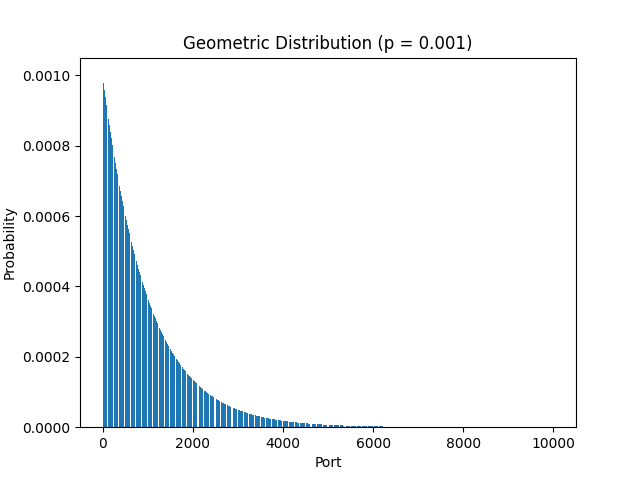
\includegraphics[width=12cm, height=7cm, keepaspectratio]{entropy/img/geometric_distribution_1000.png}
    \caption{Geometric Distribution 1,000 ports}
    \label{fig:geometric_distribution_1000}
\end{minipage}
\hspace{1.5cm}
\begin{minipage}{.45\textwidth}
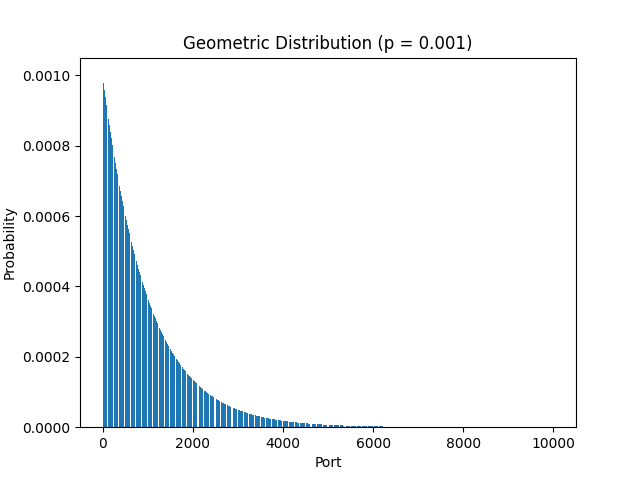
\includegraphics[width=12cm, height=7cm, keepaspectratio]{entropy/img/geometric_distribution_10000.png}
    \caption{Geometric Distribution 10,000 ports}
    \label{fig:geometric_distribution_10000}
\end{minipage}
\end{adjustwidth}
\end{figure}

\subsubsection{Zipf Distribution}

The Zipf distribution is another candidate to represent the distribution of open ports. This distribution is known for modeling scenarios where a small number of items (in our case, ports) are highly popular, while the rest have diminishing popularity. This distribution is useful for simulating scenarios where a small set of ports are commonly open, possibly mirroring common applications and services. This is similar to the geometric distribution, but the distribution is slightly different, which can be seen in the corresponding Figures~\ref{fig:zipf_distribution_1000} and~\ref{fig:zipf_distribution_10000}. 

This distribution aligns the most with our limit dataset. We believe that a distribution resembling the Zipf or Geometric distribution is more plausible in a real-world scenario. This is because certain software applications are more prevalent than others and tend to dominate in terms of usage. Additionally, the fact that many applications cannot be detected through browser-based port scanning further increases the likelihood of these popular applications being even more prevalent.

\begin{figure}[h]
\begin{adjustwidth}{-3cm}{-1cm}
\centering
\begin{minipage}{.45\textwidth}
  \centering
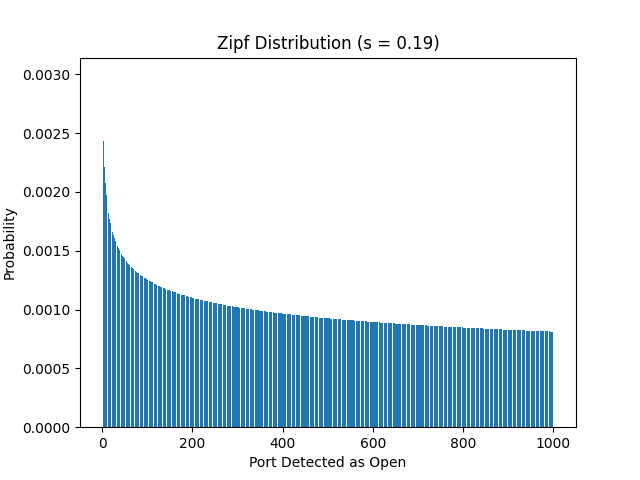
\includegraphics[width=12cm, height=7cm, keepaspectratio]{entropy/img/zipf_distribution_1000.png}
    \caption{Zipf Distribution 1,000 ports}
    \label{fig:zipf_distribution_1000}
\end{minipage}
\hspace{1.5cm}
\begin{minipage}{.45\textwidth}
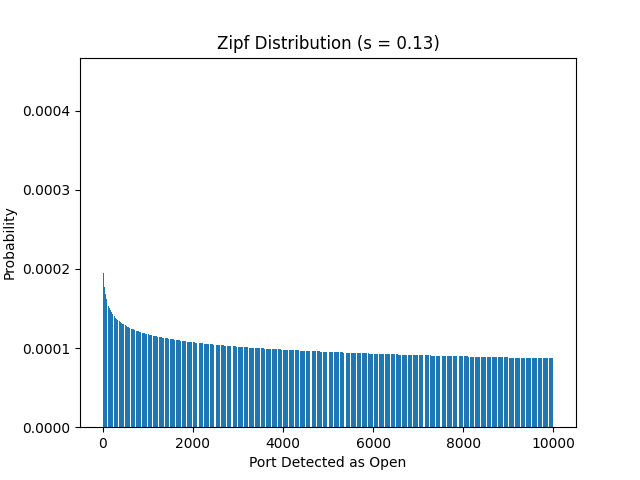
\includegraphics[width=12cm, height=7cm, keepaspectratio]{entropy/img/zipf_distribution_10000.png}
    \caption{Zipf Distribution 10,000 ports}
    \label{fig:zipf_distribution_10000}
\end{minipage}
\end{adjustwidth}
\end{figure}

\subsubsection{Uniform Distribution}

In contrast to the previous two distributions, we include the Uniform distribution to serve as a baseline comparison. In this scenario, all ports are equally likely to be open, which is an unlikely real-world situation but provides insight into what happens to entropy when all ports have equal popularity.

\section{Experiment Setup}

We use a systematic approach to investigate the relationship between data distribution and fingerprint uniqueness. 

\begin{itemize}
\item \textbf{Port Range:} For our experiments, we consider a range of 1,000 and 10,000 ports, representing a subset of the total 65,535 ports available. This choice is based on practical considerations, as scanning all 65,535 ports is time-consuming and not realistic for browser-based port scanning.

\item \textbf{Probability Distribution:} For each of the three selected probability distributions (Geometric, Zipf, Uniform), we calculate the probabilities of individual ports being open based on the chosen distribution. 
\end{itemize}

\subsubsection{Generation of Synthetic Fingerprint Datasets}

In order to properly use Shannon's entropy formula, we have to consider \emph{all possible outcomes}. Calculating all possible outcomes with such a large dataset, i.e. $2^{1000} \approx 1.07 \times 10^{301}$ takes too much time, and therefore we have two possible solutions to calculate entropy:

\begin{itemize}
    \item Sampling from the dataset, i.e. Monte Carlo simulations.
    \item Calculating entropy based on the probability distribution
\end{itemize}

We chose option 2, because sampling from such a large dataset is statistically insignificant, and we can estimate a good average entropy based on the probability distributions.
We use the python NumPy library to calculate the probabilities.

% We begin by generating synthetic fingerprint datasets to serve as the basis for our analysis. To achieve this, we utilize several probability distributions that we estimate to reflect real-world scenarios. These distributions are chosen to simulate various patterns of data distribution. 

% When we refer to data distribution, we are describing the likelihood of each port being open. Certain ports will be detected as open more frequently than others, due to variations in the popularity of the underlying applications. Our goal is to capture this popularity disparity by utilizing different distribution formulas.



\subsubsection{Investigation of Scenario Variations}

We proceed to investigate how different scenarios, represented by variations in the synthetic data, impact the levels of entropy. By introducing changes in the data distribution, we aim to understand how the uniqueness of fingerprints is influenced under various conditions.

\subsubsection{Analysis and Interpretation of Results}

Finally, we analyze and interpret the results obtained from the entropy calculations. Through this analysis, we draw conclusions regarding the relationship between data distribution patterns and the uniqueness of fingerprints. 


% \section{Experiment design}






% \subsection{Entropy Calculation}

% Based on the probabilities of the distributions, we can calculate the entropy using Shannon's entropy formula. This quantifies the uncertainty or randomness in the dataset and provides a measure of fingerprint uniqueness.

% \subsection{Statistical Analysis}

% After conducting the experiments, we perform statistical analysis to identify trends and patterns in the entropy values under various scenarios. We aim to draw conclusions about how changes in data distribution, dataset size, and port range impact fingerprint uniqueness.

% By following this experiment setup, we can gain valuable insights into the relationship between data distribution and the entropy of browser-based port scanning fingerprints, which is crucial for understanding user privacy implications and potential countermeasures.

\section{Results}

In this section, we present the results of our experiments, where we investigated the entropy of synthetic fingerprint datasets generated under different probability distributions: Geometric, Zipf, and Uniform. We varied parameters such as the number of open ports, dataset size, and the range of ports to understand their impact on fingerprint uniqueness.

\subsection{Geometric Distribution}

Under the Geometric distribution, we explored two scenarios:

\subsubsection{Scenario 1: 1,000 Ports}

\begin{itemize}
\item \textbf{Number of Ports Scanned (\(N\)):} 1,000.
\item \textbf{Average Number of Open Ports (\(k\)):} 5.
\item \textbf{Probability of Success (\(p\)):} Calculated as the average number of open ports divided by the total number of ports (\(p = \frac{k}{N}\)).
\end{itemize}

\subsubsection{Scenario 2: 10,000 Ports}

\begin{itemize}
\item \textbf{Number of Ports Scanned (\(N\)):} 10,000.
\item \textbf{Average Number of Open Ports (\(k\)):} 10.
\item \textbf{Probability of Success (\(p\)):} Calculated as the average number of open ports divided by the total number of ports (\(p = \frac{k}{N}\)).
\end{itemize}

With these parameters, the calculated entropy was approximately 9.02 for 1,000 port scans, and 11.41 for 10,000 port scans.

\subsection{Zipf Distribution}

Under the Zipf distribution, we also explored two scenarios:

\subsubsection{Scenario 1: 1,000 Ports}

\begin{itemize}
\item \textbf{Number of Ports Scanned (\(N\)):} 1,000.
\item \textbf{Average Number of Open Ports (\(k\)):} 5.
\item \textbf{Exponent Parameter (\(s\)):} Governs the distribution's skewness. Calculated as \(s \approx \frac{1}{\ln(\frac{N}{k})}\) to achieve a similar level of port popularity as in the Geometric Distribution.
\end{itemize}

\subsubsection{Scenario 2: 10,000 Ports}

\begin{itemize}
\item \textbf{Number of Ports Scanned (\(N\)):} 10,000.
\item \textbf{Average Number of Open Ports (\(k\)):} 10.
\item \textbf{Exponent Parameter (\(s\)):} Governs the distribution's skewness. Calculated as \(s \approx \frac{1}{\ln(\frac{N}{k})}\) to achieve a similar level of port popularity as in the Geometric Distribution.
\end{itemize}

With these parameters, the calculated entropy was approximately 9.93 for 1,000 port scans, and 13.27 for 10,000 port scans.


\subsection{Uniform Distribution}

Under the Uniform distribution, we considered two scenarios:

\subsubsection{Scenario 1: 1,000 Ports}

\begin{itemize}
\item \textbf{Number of Ports Scanned (\(N\)):} 1,000.
\end{itemize}

\subsubsection{Scenario 2: 10,000 Ports}

\begin{itemize}
\item \textbf{Number of Ports Scanned (\(N\)):} 10,000.
\end{itemize}

With these parameters, the calculated entropy was approximately 9.96 for 1,000 ports, and 13.29 for 10,000 ports.

\section{Analysis}

In this section, we analyze the results obtained from the experiment. We compare the differences in entropy when we increase the number of ports scanned (from 1,000 to 10,000) while also taking into account the variations in entropy resulting from different probability distributions. 

\subsubsection{Comparison Between Geometric and Zipf Distributions}

One of the central aspects of the experiment is comparing the Geometric and Zipf distributions in terms of their impact on fingerprint uniqueness. Our findings reveal the following insights: When comparing the Geometric and Zipf distributions, we observe notable differences in the resulting entropy values. Under similar scenarios, the Zipf distribution consistently yields higher entropy compared to the Geometric distribution. This demonstrates the impact of distribution skewness on fingerprint complexity. 

As logically follows, due to the Zipf distribution being more uniform than the Geometric distribution, the uniqueness of the Zipf distribution is higher. This means that if the popularity of certain applications is not as prevalent as we think it is, the entropy will be even more unique. Nevertheless, the Geometric distribution already gives 9 bits of entropy within 1 second of port scanning (1,000 ports).

\subsubsection{Impact of Increased Search Space}

Another aspect we explored is the influence of expanding the search space by increasing the number of ports scanned.
For the Geometric distribution, transitioning from scanning 1,000 ports with 5 average open ports (Scenario 1) to scanning 10,000 ports with 10 average open ports (Scenario 2) resulted in a relatively modest increase in entropy, approximately 2.39 bits. This suggests that, for the Geometric distribution, the search space expansion had a more incremental effect on fingerprint uniqueness.
In contrast, the Zipf distribution exhibited a more substantial impact when transitioning between scenarios. The entropy increased by approximately 3.34 bits, emphasizing that the Zipf distribution's effectiveness in generating unique fingerprints becomes more pronounced with a larger search space.

On certain webpages where a user is expected to stay for a longer time, the search space can be expanded to a higher number. When 1,000 ports are mapped to the most popular applications currently opening a port, browser-based port scanning becomes a realistic and powerful fingerprinting technique. Especially when ports outside the dynamic port range are scanned, browser-based port scanning can be utilized for user-tracking, as most ports will not be ephemeral.

It is important to emphasize that while a user is navigating a website, browser-based port scanning can continue without interruption. A sophisticated scanning mechanism can efficiently scan, and at the same time, relay the scan results back to a server. This extends the scanning duration throughout the user's entire session on the website, which typically lasts much longer than one second. As a result, the search space can easily be expanded to accommodate up to 10,000 ports or higher, depending on the website. The larger the search space, the higher the entropy will be.

\subsubsection{Uniform Distribution Comparison}

We also compared the Uniform distribution with both distributions.
Notably, the Uniform distribution exhibited similar entropy values to the Zipf distribution under similar scenarios, despite the difference in the probability of detecting open ports.

\subsubsection{Real world validation}

We have integrated port-scanning within the popular FingerprintJS~\citeartifact{fingerprintjs} library, and we assessed that 1,000 ports can easily be scanned on any webpage, together with existing fingerprinting techniques, without noticeable impact on the end user. 


\section{Conclusion}

In conclusion, our experiments show that browser-based port scanning is a realistic threat to user anonymity on the internet, based on our assumptions. We have examined the impact of different probability distributions (Geometric, Zipf, and Uniform) and the expansion of search space on the entropy of fingerprints generated through port scanning.
One of the most important findings of this experiment is that regardless of the distribution used, we consistently observed high levels of entropy, indicating the potential for creating highly unique fingerprints through browser-based port scanning, within a short period of scanning time (< 1 second).

This finding suggests that a fingerprint with an entropy of at least 9 can be generated within roughly one second of scanning. When combined with existing fingerprinting techniques, such as time zone, plugins, ad blocker, user-agent, fonts, screen resolution, etc., this results in a cumulative entropy that exceeds 50 bits of entropy~\citescientific{gomez2018}. Narayanan~\citescientific{narayanan201233} argues that an entropy of 33 bits is sufficient to uniquely identify users ($2^{33}$ = 8,59 billion), emphasizing the threat that browser-based port scanning poses to user anonymity on the internet.

In light of these findings, it is evident that browser-based port scanning can be a tool for user profiling and tracking, especially when combined with existing fingerprinting techniques. As such, it is imperative for users, and more importantly browser developers, to be aware of these threats and take proactive measures to prevent unauthorized local port scanning.







% \begin{enumerate}
%   \item \textbf{Common Software Usage:} Most users run common software applications that open specific ports. This commonality reduces the variation in open port combinations.
  
%   \item \textbf{Limited Concurrent Applications:} Users typically run a limited number of applications simultaneously, further reducing the number of open ports that can be detected.
  
%   \item \textbf{Port Popularity:} Certain ports, such as those associated with popular services (e.g., email, web browsing, and messaging), are more frequently open, while others remain closed by default.
% \end{enumerate}



% https://math.stackexchange.com/questions/2729561/probability-of-an-unordered-sample-under-weighted-sampling-without-replacement




% https://dl.acm.org/doi/fullHtml/10.1145/3178876.3186097

\chapter{Conclusions and Discussion}

In this document, we researched browser-based port scanning and drew the following conclusions based on our findings: 
\\

\textbf{RQ1: How to choose the optimal port-scanning technique for a specific victim client in combination with a specific attack goal?}

We measured significant variations between different operating systems and scanning techniques. The Fetch API emerged as the most effective JavaScript API for conducting browser-based port scanning, and it proved to be highly efficient across various configurations. This can primarily be attributed to the \emph{no-cors} mode, a setting unique to the Fetch API.
A notable contrast was observed between Ubuntu and Windows. Ubuntu tended to time out network requests whenever possible, whereas Windows adhered to the configured socket timeout settings. This characteristic made browser-based port scanning considerably more efficient on Ubuntu.

We estimate that on Windows/Chrome, which is the most popular combination of OS/Browser, it is possible to scan 1,000 ports within one second (2,500+ on Ubuntu). This makes browser-based port scanning a practical real-world attack on virtually any web page. This is especially concerning because the scanning process can continue throughout a user's entire session on the website, which usually lasts much longer than just one second. 
\\

\textbf{RQ2: What information can browser-based port scanning reveal about the underlying operating system?}

We found that operating systems by default do not expose ports that can be revealed through a browser, with the exception of CUPS on Ubuntu. 
Most OS ports fall under the restricted port range and cannot be detected through browser-based port scanning. 
However, when activating certain services on the OS, some of these services are detectable, such as Hyper-V on Windows.
Furthermore, both Windows and Ubuntu host a \texttt{/etc/services} file which contains a mapping between ports and OS services. This mapping can be used as a foundation for a targeted scan to fingerprint the underlying OS.
\\

\textbf{RQ3: What information can browser-based port scanning reveal about specific programs
running locally on a user’s system?}

Fingerprinting specific programs is more effective than fingerprinting the OS. 
We found many programs from different categories that open a distinct port on the local system, which can be revealed through browser-based port scanning. 
We argue that browser-based port scanning can be used to track users by identifying open ports corresponding to specific applications, and is thereby a direct threat to user privacy/anonymity on the internet, especially when combined with known fingerprinting techniques.

When we can successfully identify open ports and the associated programs, it provides a detailed user profile that can be used for a multitude of purposes. 
These can include personalized web pages or more nefarious use cases such as phishing attempts.
Additionally, this information could be exploited to scan for known exploits of specific programs. 
In essence, the knowledge gained from these open ports not only undermines user privacy, but also establishes a foundation for a range of potentially malicious activities.
\\

\textbf{RQ4: How unique are browser-based port scanning fingerprints?}

We estimate that browser-based port scanning results in highly unique fingerprints, even with a very limited scanning time of only one second. We emphasize that if a mapping between the top 1,000 most popular applications and their corresponding identifiable ports is established, then scanning these 1,000 ports is sufficient to create highly unique fingerprints. These fingerprints would possess an entropy that exceeds 50 when combined with established fingerprinting techniques, which is theoretically enough to uniquely identify any user.

It is essential to note that these results are based on our estimates, and a large-scale real-world study would be necessary to validate these claims in a real-world setting. Nonetheless, we believe that our estimates are not implausible, thousands of ports being either open or closed is a significant characteristic that has been omitted from all existing browser fingerprinting studies, and would greatly enhance these fingerprints.


\subsubsection{Browser-based port scanning is a threat to user privacy and security}

The practice of browser-based port scanning poses a significant threat to user privacy. We argue that browser-based port scanning should be banned by web browsers, or at the very least, users should have to explicitly grant permissions for a website to access their local network. 
We contend that any potential benefits, such as the detection of remote access tools for comprised devices as a security measure, are outweighed by the risks to user privacy and security.
Additionally, we think that using browser-based port scanning as a security measure is inherently insufficient, and there are better --- less intrusive --- established alternatives such as multi-factor authentication, which can prevent hijacked devices from making unauthorized requests.

While the potential defensive mechanism of browser-based port scanning is insufficient, the threats are real.
We established the following threats to privacy in this paper:
\begin{itemize}
    \item Identification of specific open ports: Browser-based port scanning can be used to scan specific ports on a system, corresponding to an application natively opening that specific port. This knowledge can be leveraged to target users who are utilizing a particular type of application or service.
    \item Highly unique fingerprints: Browser-based port scanning, combined with existing fingerprinting techniques, can create highly unique fingerprints, effectively eliminating user anonymity on the internet.
\end{itemize}

While not a focus of this paper, the threats to security are also a significant consideration:
\begin{itemize}
    \item Drive-By Pharming~\citescientific{stamm2007}: Drive-by Pharming was an attack in which a malicious web page, when visited, attempted to change a victim's router DNS settings to gain control over their internet traffic and potentially compromise their credentials.
    \item SOHO Pharming~\citetechnical{sohopharming2013}: SOHO Pharming was an attack that compromised over 300,000 consumer-grade SOHO routers, primarily in Europe and Asia since December 2013. Attackers manipulated DNS configurations, redirected DNS requests, and performed Man-in-the-Middle attacks. The attack targeted various router models, exploited vulnerabilities such as authentication bypass and CSRF techniques, and took advantage of consumer unfamiliarity with router configurations and insecure default settings.
\end{itemize}

\subsubsection{Opt-In Solution for Enhanced Privacy and Security}

The only real benefit to accessing the local network would be a website integrating with its native desktop application. 
Granting explicit permission for this access aligns with established practices for various resources accessed by browsers, such as microphones and cameras.
The Brave browser has already implemented this functionality on both their desktop and mobile browser~\citearticle{brave_localhost}. 
We argue that more mainstream browsers such as Chrome, Firefox, Safari and Edge should adopt this change and give users more control over their privacy. 

West and Rigoudy~\citetechnical{rigoudy2023} have worked on a draft specification to prevent unauthorized private network access from the public internet. 
While this specification is still in draft and not on track to be a W3C standard, we think it should be. 
The principle of least privilege is becoming more popular in modern software architecture. 
Software developed (i.e. browsers) for end users should embrace this principle. 
By adopting the principle of least privilege, software can ensure that users are protected by default, rather than exposed to external threats by default, making it clear that the opt-in approach should be the standard for safeguarding user security and privacy.

In the current landscape, users have several options available to protect themselves against browser-based port scanning. 
One approach involves choosing browsers prioritizing user consent, like the Brave browser. 
However, transitioning to a new browser might pose usability challenges despite its emphasis on privacy.
Another strategy revolves around disabling JavaScript, a step effective in enhancing privacy, but detrimental to modern webpage functionality.
A more realistic alternative is a browser extension, such as the open source \emph{LAN Port Scan Forbidder}~\citeartifact{lanportscanforbidder}. 
This extension prevents unauthorized access to local networks. 
Nevertheless, relying on these measures highlights the conflict between privacy and usability and underscores the need for default user privacy in online environments.
Advocating for a shift where user privacy and security are default settings in modern web browsers remains crucial. 
This approach would alleviate the need for users to resort to these measures and promote a more user-centric approach to online privacy.

\clearpage


\section{Future work}

\subsubsection{Real-world validation}

As we have demonstrated that browser-based port scanning can be used to enhance existing fingerprinting methods and create unique fingerprints, a logical follow-up would be to assess its potential for user-tracking in a real world setting.
The ability to identify and track individuals across various online services and platforms has far-reaching consequences, affecting not only personal privacy but also the potential for data abuse and exploitation.

Existing fingerprinting techniques can already identify users up to a certain point. However, as demonstrated in previous chapters, browser-based port scanning can enhance the uniqueness of existing fingerprinting techniques, and can thereby increase the capabilities of user-tracking.
To evaluate the potential of browser-based port scanning in this regard, conducting a large-scale user study becomes necessary. Such a study would gauge the effectiveness of user-tracking capabilities in a real world setting, when browser-based port scanning is incorporated with existing fingerprinting techniques.

\subsubsection{Scanning private networks}

In our research, we primarily concentrated on using browser-based port scanning to scan the localhost IP address. This focus was chosen because browser-based port scanning is a time-intensive process, and the localhost IP address will generally be the most interesting IP address to scan. However, it is important to note that browser-based port scanning can be extended to scan other private IP addresses, which may reveal sensitive information.

\subsubsection{Browser-based port scanning on mobile}

Preliminary research was conducted on using browser-based port scanning to scan mobile devices. The initial findings did not yield any significant discoveries, but there exists potential for further exploration in this area, as the preliminary research was surface-level and did not dive deep into the network layer.
Mobile devices have become a primary means of accessing online services and platforms for a significant portion of the population. Understanding how browser-based port scanning behaves on mobile platforms is important, as it may have unique implications and challenges compared to desktop environments.

\subsubsection{Unsafe ports}
As mentioned in our research, unsafe or restricted ports refer to a range of ports that are blocked by the browser.
No information can be obtained from these ports, and this is a big limitation of browser-based port scanning. 
Critical ports hosting OS services such as FTP, SSH, and SMTP are protected by this rule, and we cannot obtain information about them.
However, as described in the documentation by Mozilla~\cite{firefox_restricted_ports}, there are protocol specific exceptions that are able to access these ports, such as the FTP, POP3 and IMAP protocols.
Leveraging these protocols or finding a different way to bypass the restriction of unsafe ports is a topic for further exploration. 


% \section{Discussion}
% Here, you discuss everything that might be questionable about your research. Try to be very honest, and discuss everything that makes that the results are not 100\% reliable.

% You may also make the discussion a subsection in your Conclusions.

% Check whether the best place for the discussion is before or after the Conclusions.

%% \backmatter{}
% \chapter{Reflection}
% It is appreciated when you ad a personal reflection on your graduation process. What did you learn? How did the process go?

% When you add such a chapter, you deliver two versions: one with the relfection, for your supervisors, and one without, for public access.

\bibliographystyle{alpha}

\bibliography{report,
introduction/references/user_privacy,
introduction/references/port_scanning,
relatedwork/references/bot_detection, relatedwork/references/browser_fingerprinting, relatedwork/references/cloaking, 
relatedwork/references/port_scanning,
port_scanning_techniques/references/port_scanning_techniques,
entropy/entropy
}


%% Use letters for the chapter numbers of the appendices.
%\appendix
\appendix
\chapter{Appendix A: Scanning techniques comparison}
\pagenumbering{roman}
\label{appendix:appendix-a}

\section{Experiment Parameters}
\label{appendix:expirement-parameters}
%% \begin{figure}[ht]
%% \begin{tabular}{p{5cm}p{5cm}p{5cm}}
\begin{itemize}
\item Operating system:
    \begin{itemize}
    \item Windows 10.0.19042.1889
    \item Ubuntu 22.04 (LTS)
    \end{itemize}
\item Browser:
    \begin{itemize}
    \item Chrome 114.0.5735.91
    \item FireFox 115.0.2
    \end{itemize}
\item Scanning technique:
    \begin{itemize}
    \item Fetch
    \item XHR
    \item WebSocket
    \end{itemize}
\item Socket settings:
    \begin{itemize}
    \item Parallel sockets: 1, 5, 10, 20, 30, 40, 50, 60, 70, 100, 150, 200, 250
    \item Socket timeout settings: 100ms, 150ms, 200ms, 250ms, 300ms, 400ms 
    \end{itemize}
\item Artificially opened ports:
    \begin{itemize}
    \item N HTTP servers: 10, 33, 50, 100
    \end{itemize}
\end{itemize}

\clearpage
\section{Socket timeout comparison}

\begin{table}[htbp]
\footnotesize
\centering
\begin{adjustwidth}{-1.0cm}{}
\begin{tabular}{p{6.3cm}p{1.5cm}p{3cm}p{2cm}p{2cm}}
    \toprule
    Base Image & Browser & Socket timeout (ms) & Scanning Technique & Detected ports \\
     \midrule
    mcr.microsoft.com/windows:20H2-amd64 & Chrome & 100 & Fetch & 76 \\
    mcr.microsoft.com/windows:20H2-amd64 & Chrome & 150, 200, 250, 300, 350, 400 & Fetch & 100 \\
    mcr.microsoft.com/windows:20H2-amd64 & Chrome & 100, 150, 200, 250, 300, 350, 400, 1000 & WebSocket, XHR & 0 \\
    \midrule
    mcr.microsoft.com/windows:20H2-amd64 & Firefox & 100 & Fetch & 21 \\
    mcr.microsoft.com/windows:20H2-amd64 & Firefox & 150, 200, 250, 300, 350, 400 & Fetch & 100 \\
    mcr.microsoft.com/windows:20H2-amd64 & Firefox & 100, 150, 200, 250, 300, 350, 400, 1000 & WebSocket, XHR & 0 \\
    \midrule
    library/ubuntu:22.04 & Chrome & 100, 150, 200, 250, 300, 350, 400 & Fetch & 100 \\
    library/ubuntu:22.04 & Chrome & 100, 150, 200, 250, 300, 350, 400 & WebSocket, XHR & 0 \\
    \midrule
    library/ubuntu:22.04 & Firefox & 100, 150, 200, 250, 300, 350, 400 & Fetch & 100 \\
    library/ubuntu:22.04 & Firefox & 100, 150, 200, 250, 300, 350, 400 & WebSocket, XHR & 0 \\
     \bottomrule
\end{tabular}
\end{adjustwidth}{}
\caption{Number of ports detected based on socket timeout setting (100 open ports), scans were rerun 5 times to verify the accuracy of the results.}
\label{tab:socket-timeout-comparison}
\end{table}

\clearpage

\section{Scanning technique efficacy comparison}

\begin{table}[htbp]
    \footnotesize
    \centering
    \begin{tabular}{p{6.3cm}p{1.5cm}p{1.7cm}p{1.7cm}p{2.2cm}p{3cm}}
        \toprule
        Base Image & Scanning Technique & Open Ports & Ports Detected & Scan Duration (ms) \\
        \midrule
        mcr.microsoft.com/windows:20H2-amd64 & Fetch & 10 & 10 & 1282.6 \\
        mcr.microsoft.com/windows:20H2-amd64 & Fetch & 33 & 33 & 1313.5 \\
        mcr.microsoft.com/windows:20H2-amd64 & Fetch & 50 & 50 & 13153.8 \\
        mcr.microsoft.com/windows:20H2-amd64 & Fetch & 100 & 100 & 1177.4 \\
        \midrule
        mcr.microsoft.com/windows:20H2-amd64 & WebSocket & 10 & 0 & 1463.5 \\
        mcr.microsoft.com/windows:20H2-amd64 & WebSocket & 33 & 0 & 1454.0 \\
        mcr.microsoft.com/windows:20H2-amd64 & WebSocket & 50 & 0 & 1464.3 \\
        mcr.microsoft.com/windows:20H2-amd64 & WebSocket & 100 & 0 & 1457.1 \\
        \midrule
        mcr.microsoft.com/windows:20H2-amd64 & XHR & 10 & 0 & 1277.4 \\
        mcr.microsoft.com/windows:20H2-amd64 & XHR & 33 & 0 & 1303.3 \\
        mcr.microsoft.com/windows:20H2-amd64 & XHR & 50 & 0 & 1313.5 \\
        mcr.microsoft.com/windows:20H2-amd64 & XHR & 100 & 0 & 1097.2 \\
        \midrule
        library/ubuntu:22.04 & Fetch & 10 & 10 & 104.5 \\
        library/ubuntu:22.04 & Fetch & 33 & 33 & 133.4 \\
        library/ubuntu:22.04 & Fetch & 50 & 50 & 160.9 \\
        library/ubuntu:22.04 & Fetch & 100 & 100 & 209.4 \\
        \midrule
        library/ubuntu:22.04 & WebSocket & 10 & 0 & 1217.6 \\
        library/ubuntu:22.04 & WebSocket & 33 & 0 & 1216.5 \\
        library/ubuntu:22.04 & WebSocket & 50 & 0 & 1260.0 \\
        library/ubuntu:22.04 & WebSocket & 100 & 0 & 1216.6 \\
        \midrule
        library/ubuntu:22.04 & XHR & 10 & 0 & 98.3 \\
        library/ubuntu:22.04 & XHR & 33 & 0 & 135.3 \\
        library/ubuntu:22.04 & XHR & 50 & 0 & 154.2 \\
        library/ubuntu:22.04 & XHR & 100 & 0 & 231.9 \\
        \bottomrule
    \end{tabular}
    \caption{Scanning techniques comparison on Chrome detecting HTTP ports. 50 parallel connections, 200ms socket timeout, 300 ports scanned.}
    \label{tab:scan-technique-comparison-chrome}
\end{table}

\clearpage

\begin{table}[htbp]
    \footnotesize
    \centering
    \begin{tabular}{p{6.3cm}p{1.5cm}p{1.7cm}p{1.7cm}p{2.2cm}p{3cm}}
        \toprule
        Base Image & Scanning Technique & Open Ports & Ports Detected & Scan Duration (ms) \\
        \midrule
        mcr.microsoft.com/windows:20H2-amd64 & Fetch & 10 & 10 & 2553 \\
        mcr.microsoft.com/windows:20H2-amd64 & Fetch & 33 & 33 & 2561 \\
        mcr.microsoft.com/windows:20H2-amd64 & Fetch & 50 & 50 & 2552 \\
        mcr.microsoft.com/windows:20H2-amd64 & Fetch & 100 & 100 & 2386 \\
        \midrule
        mcr.microsoft.com/windows:20H2-amd64 & WebSocket & 10 & 0 & 2627 \\
        mcr.microsoft.com/windows:20H2-amd64 & WebSocket & 33 & 0 & 2629 \\
        mcr.microsoft.com/windows:20H2-amd64 & WebSocket & 50 & 0 & 2511 \\
        mcr.microsoft.com/windows:20H2-amd64 & WebSocket & 100 & 0 & 2284 \\
        \midrule
        mcr.microsoft.com/windows:20H2-amd64 & XHR & 10 & 0 & 2536 \\
        mcr.microsoft.com/windows:20H2-amd64 & XHR & 33 & 0 & 2569 \\
        mcr.microsoft.com/windows:20H2-amd64 & XHR & 50 & 0 & 2592 \\
        mcr.microsoft.com/windows:20H2-amd64 & XHR & 100 & 0 & 2308 \\
        \midrule
        library/ubuntu:22.04 & Fetch & 10 & 10 & 286 \\
        library/ubuntu:22.04 & Fetch & 33 & 33 & 307 \\
        library/ubuntu:22.04 & Fetch & 50 & 50 & 282 \\
        library/ubuntu:22.04 & Fetch & 100 & 100 & 299 \\
        \midrule
        library/ubuntu:22.04 & WebSocket & 10 & 0 & 268 \\
        library/ubuntu:22.04 & WebSocket & 33 & 0 & 276 \\
        library/ubuntu:22.04 & WebSocket & 50 & 0 & 290 \\
        library/ubuntu:22.04 & WebSocket & 100 & 0 & 270 \\
        \midrule
        library/ubuntu:22.04 & XHR & 10 & 0 & 254 \\
        library/ubuntu:22.04 & XHR & 33 & 0 & 297 \\
        library/ubuntu:22.04 & XHR & 50 & 0 & 287 \\
        library/ubuntu:22.04 & XHR & 100 & 0 & 307 \\
        \bottomrule
    \end{tabular}
    \caption{Scanning techniques comparison on Firefox detecting HTTP ports. 50 parallel connections, 400ms timeout, 300 ports scanned.}
    \label{tab:scan-technique-comparison-firefox}
\end{table}

Note that the results in Tables~\ref{tab:scan-technique-comparison-chrome} and~\ref{tab:scan-technique-comparison-firefox} do not mark ports as detected if they can be detected through post-scan analysis. The next section showcases the ability to detect open ports through post-scan analysis.


\section{Post-scan analysis efficacy comparison}
\label{appendix:scan-duration-comparison}
Scanning technique comparison through post-scan analysis. Comparing response times between open and closed ports.

\begin{figure}[ht]
\centering
\begin{minipage}{.45\textwidth}
  \centering
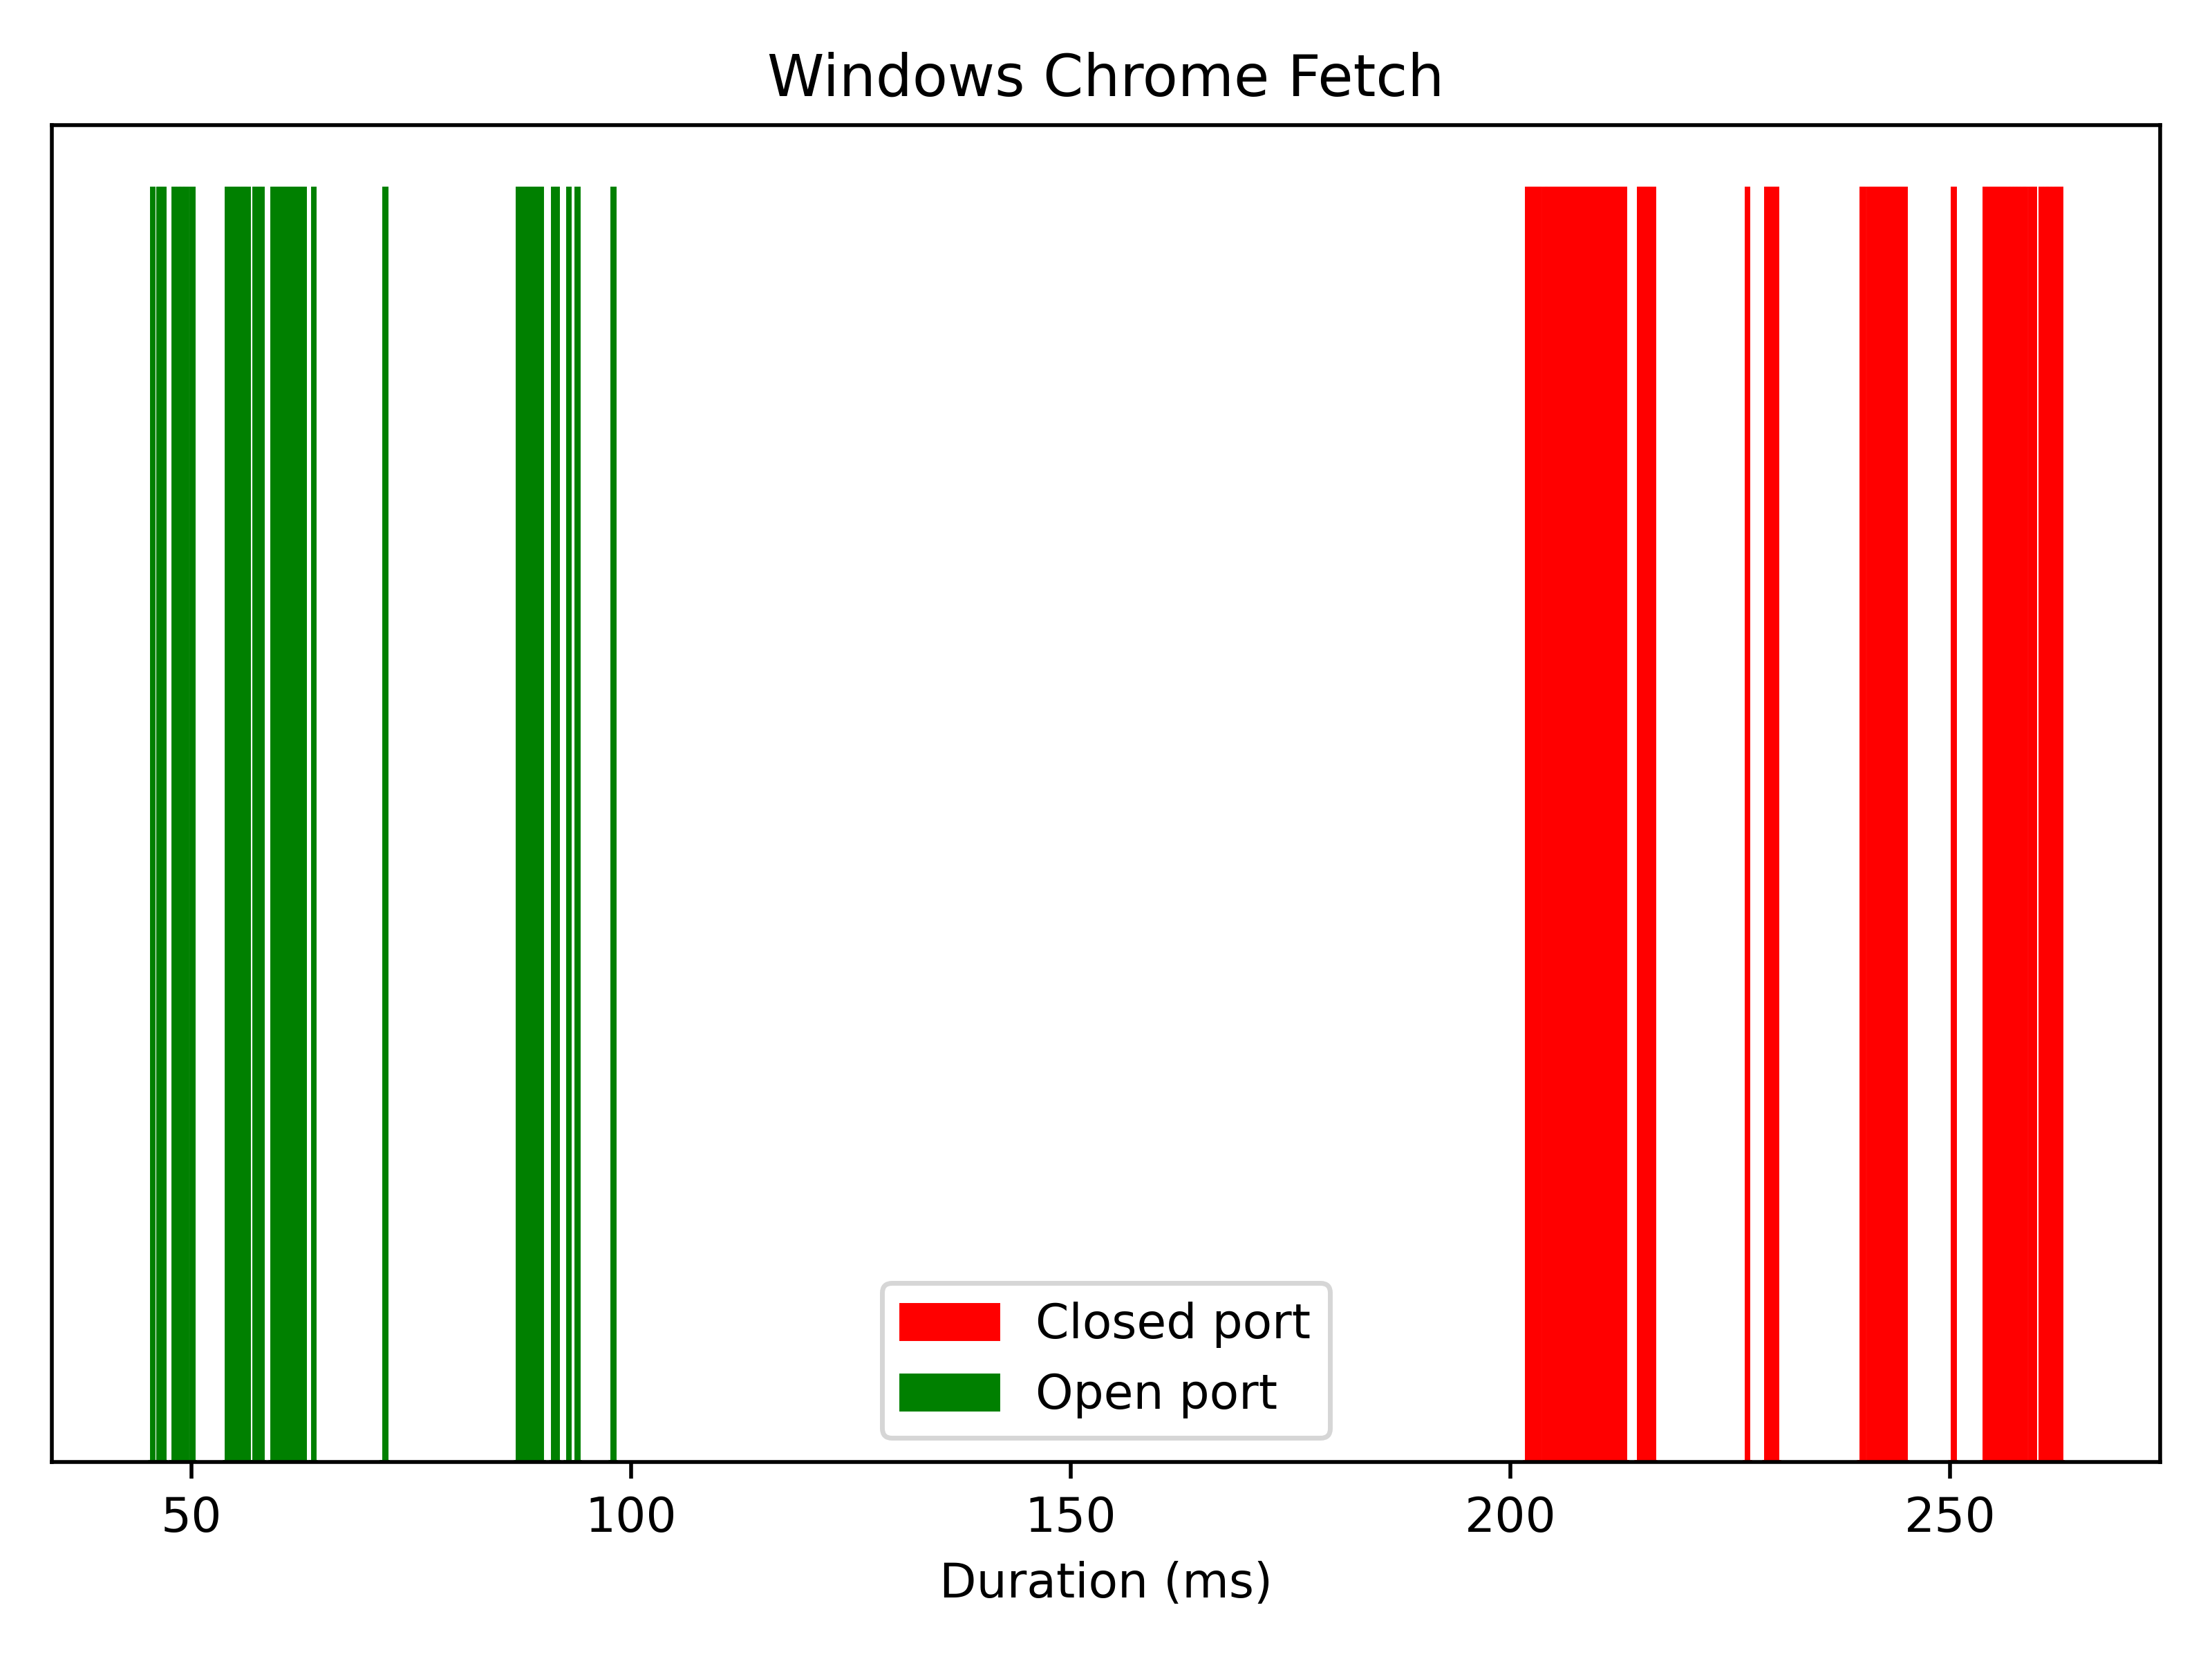
\includegraphics[width=8cm, height=4cm, keepaspectratio]{port_scanning_techniques/img/windows_chrome_efficacy_fetch.png}
    \caption{Windows/Chrome Fetch API scan duration open vs closed ports}
    \label{fig:win-chrome-fetch}
\end{minipage}
\hspace{0.5cm} % Adjust the horizontal space between the two figures
\begin{minipage}{.45\textwidth}
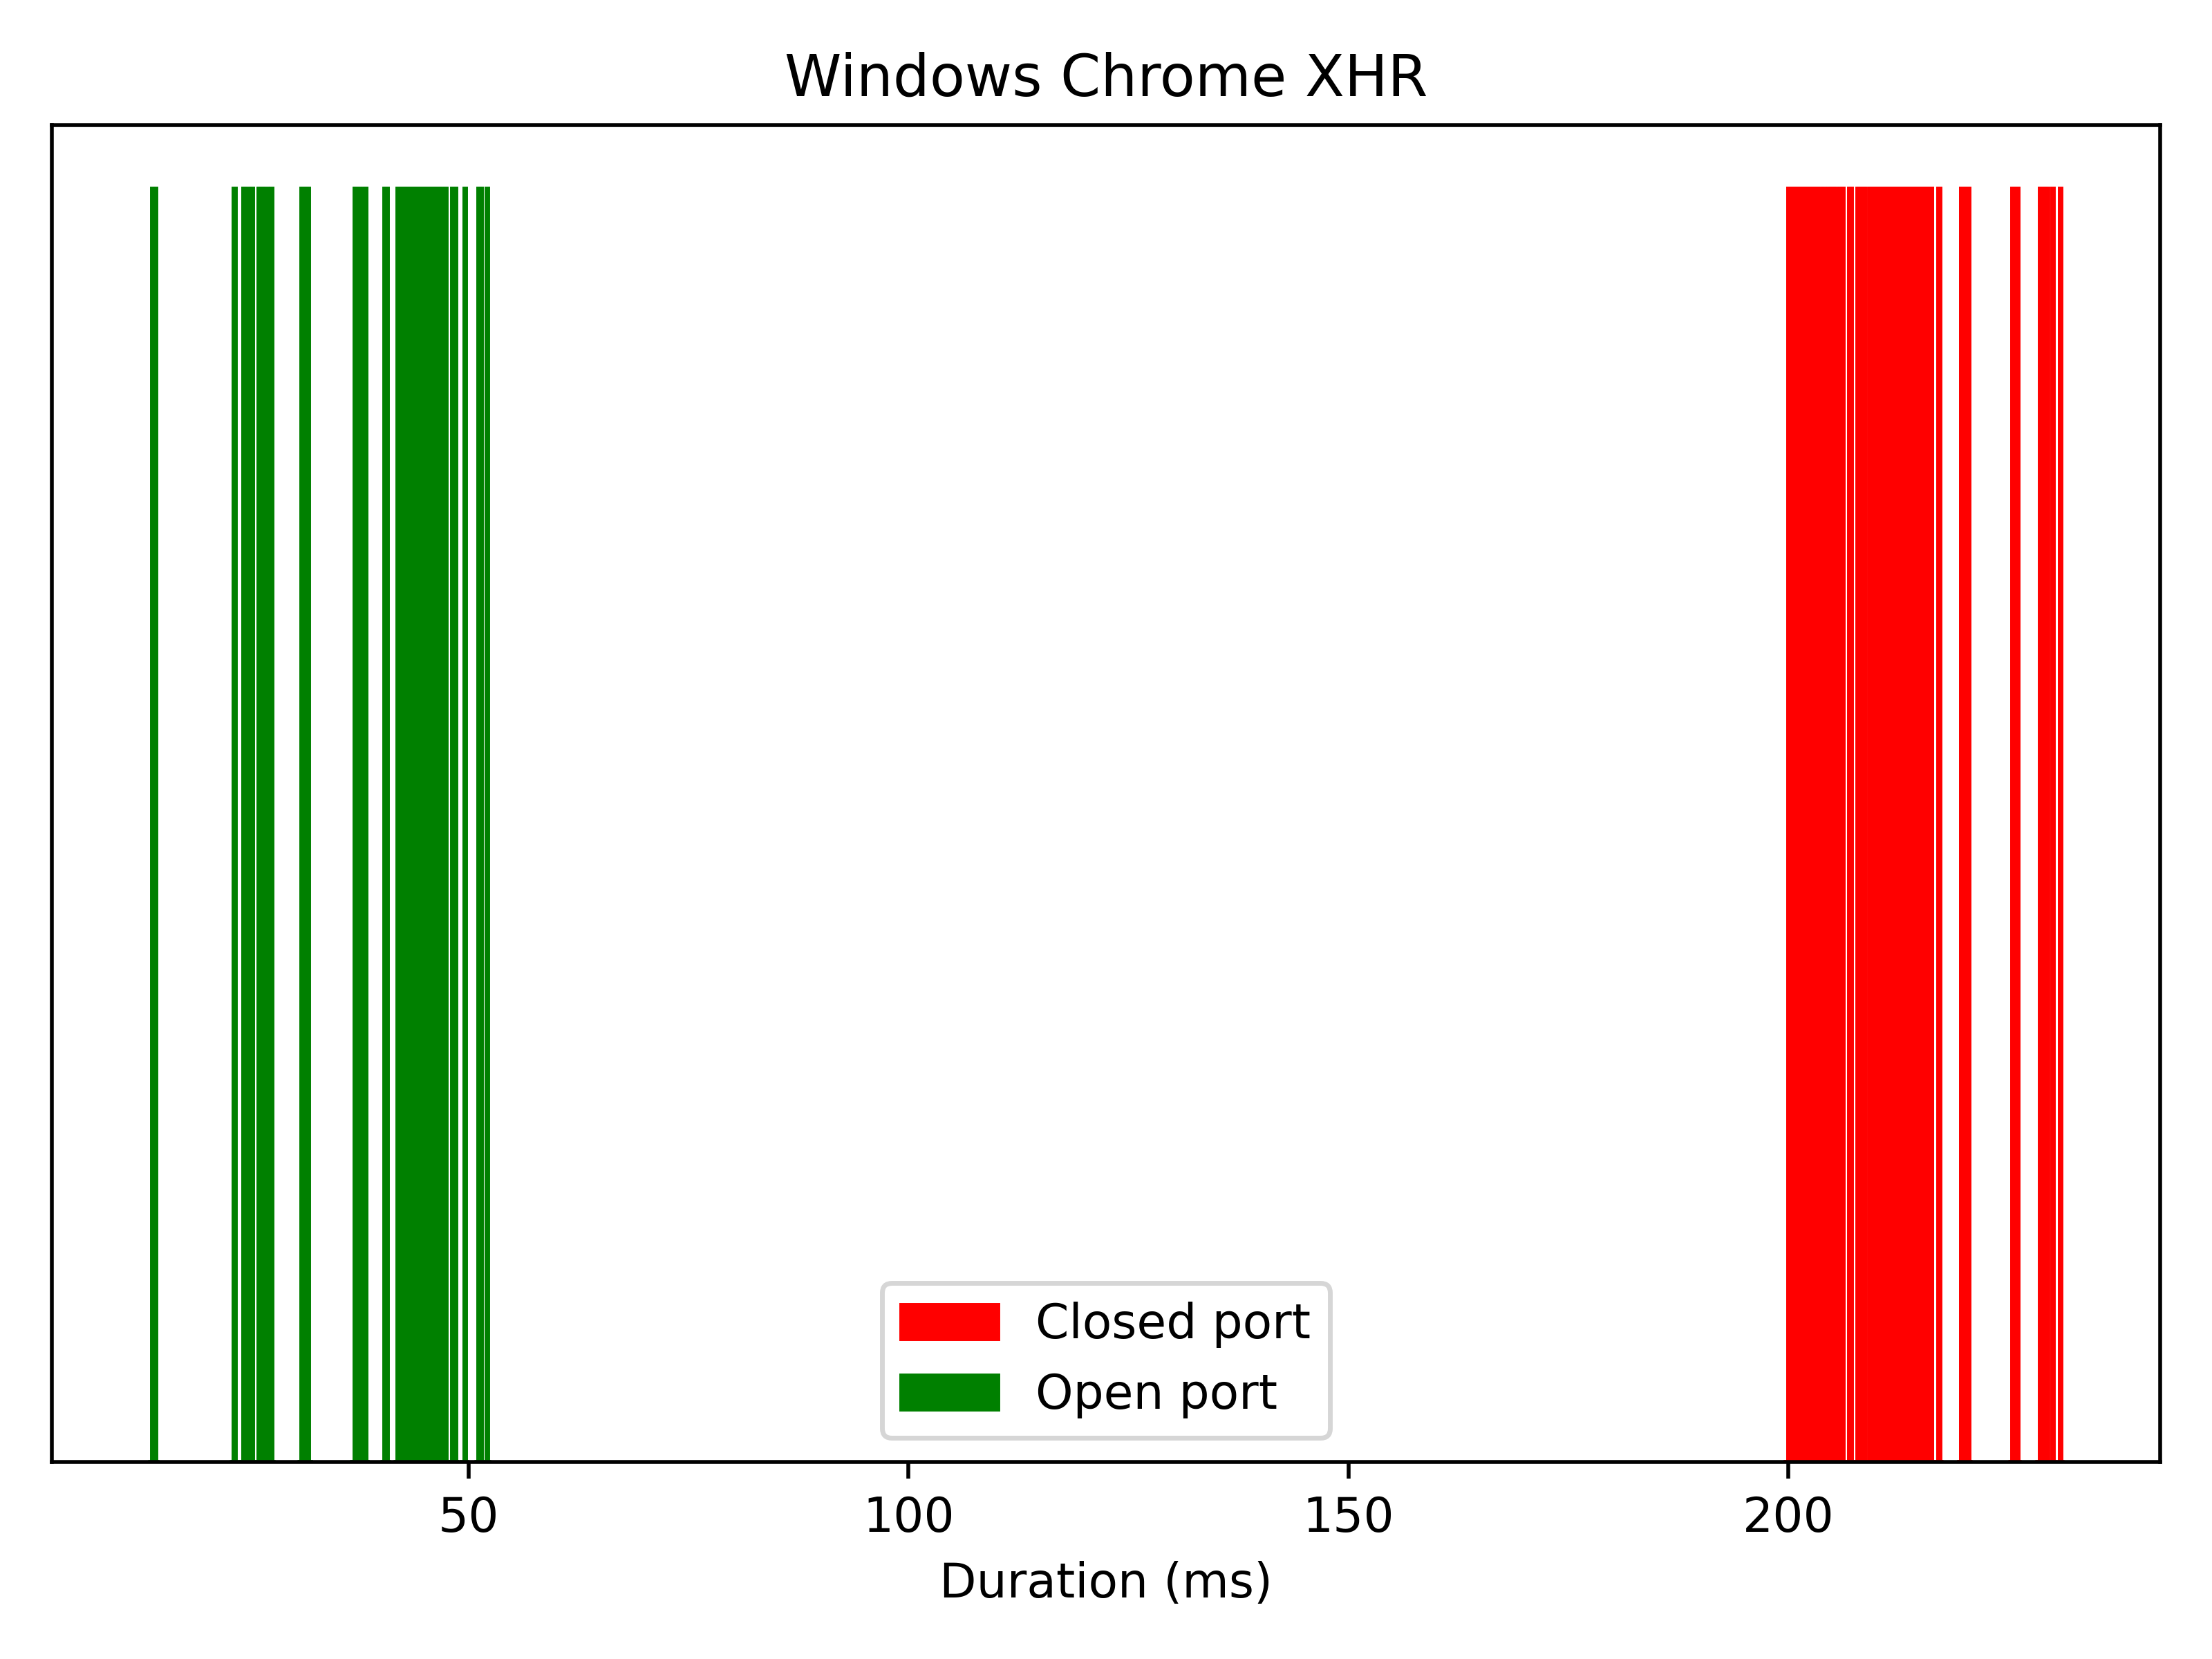
\includegraphics[width=8cm, height=4cm, keepaspectratio]{port_scanning_techniques/img/windows_chrome_efficacy_xhr.png}
    \caption{Windows/Chrome XHR API scan duration open vs closed ports}
    \label{fig:appendix-win-chrome-xhr}
\end{minipage}
\end{figure}

\begin{figure}[ht]
\centering
\begin{minipage}{.45\textwidth}
  \centering
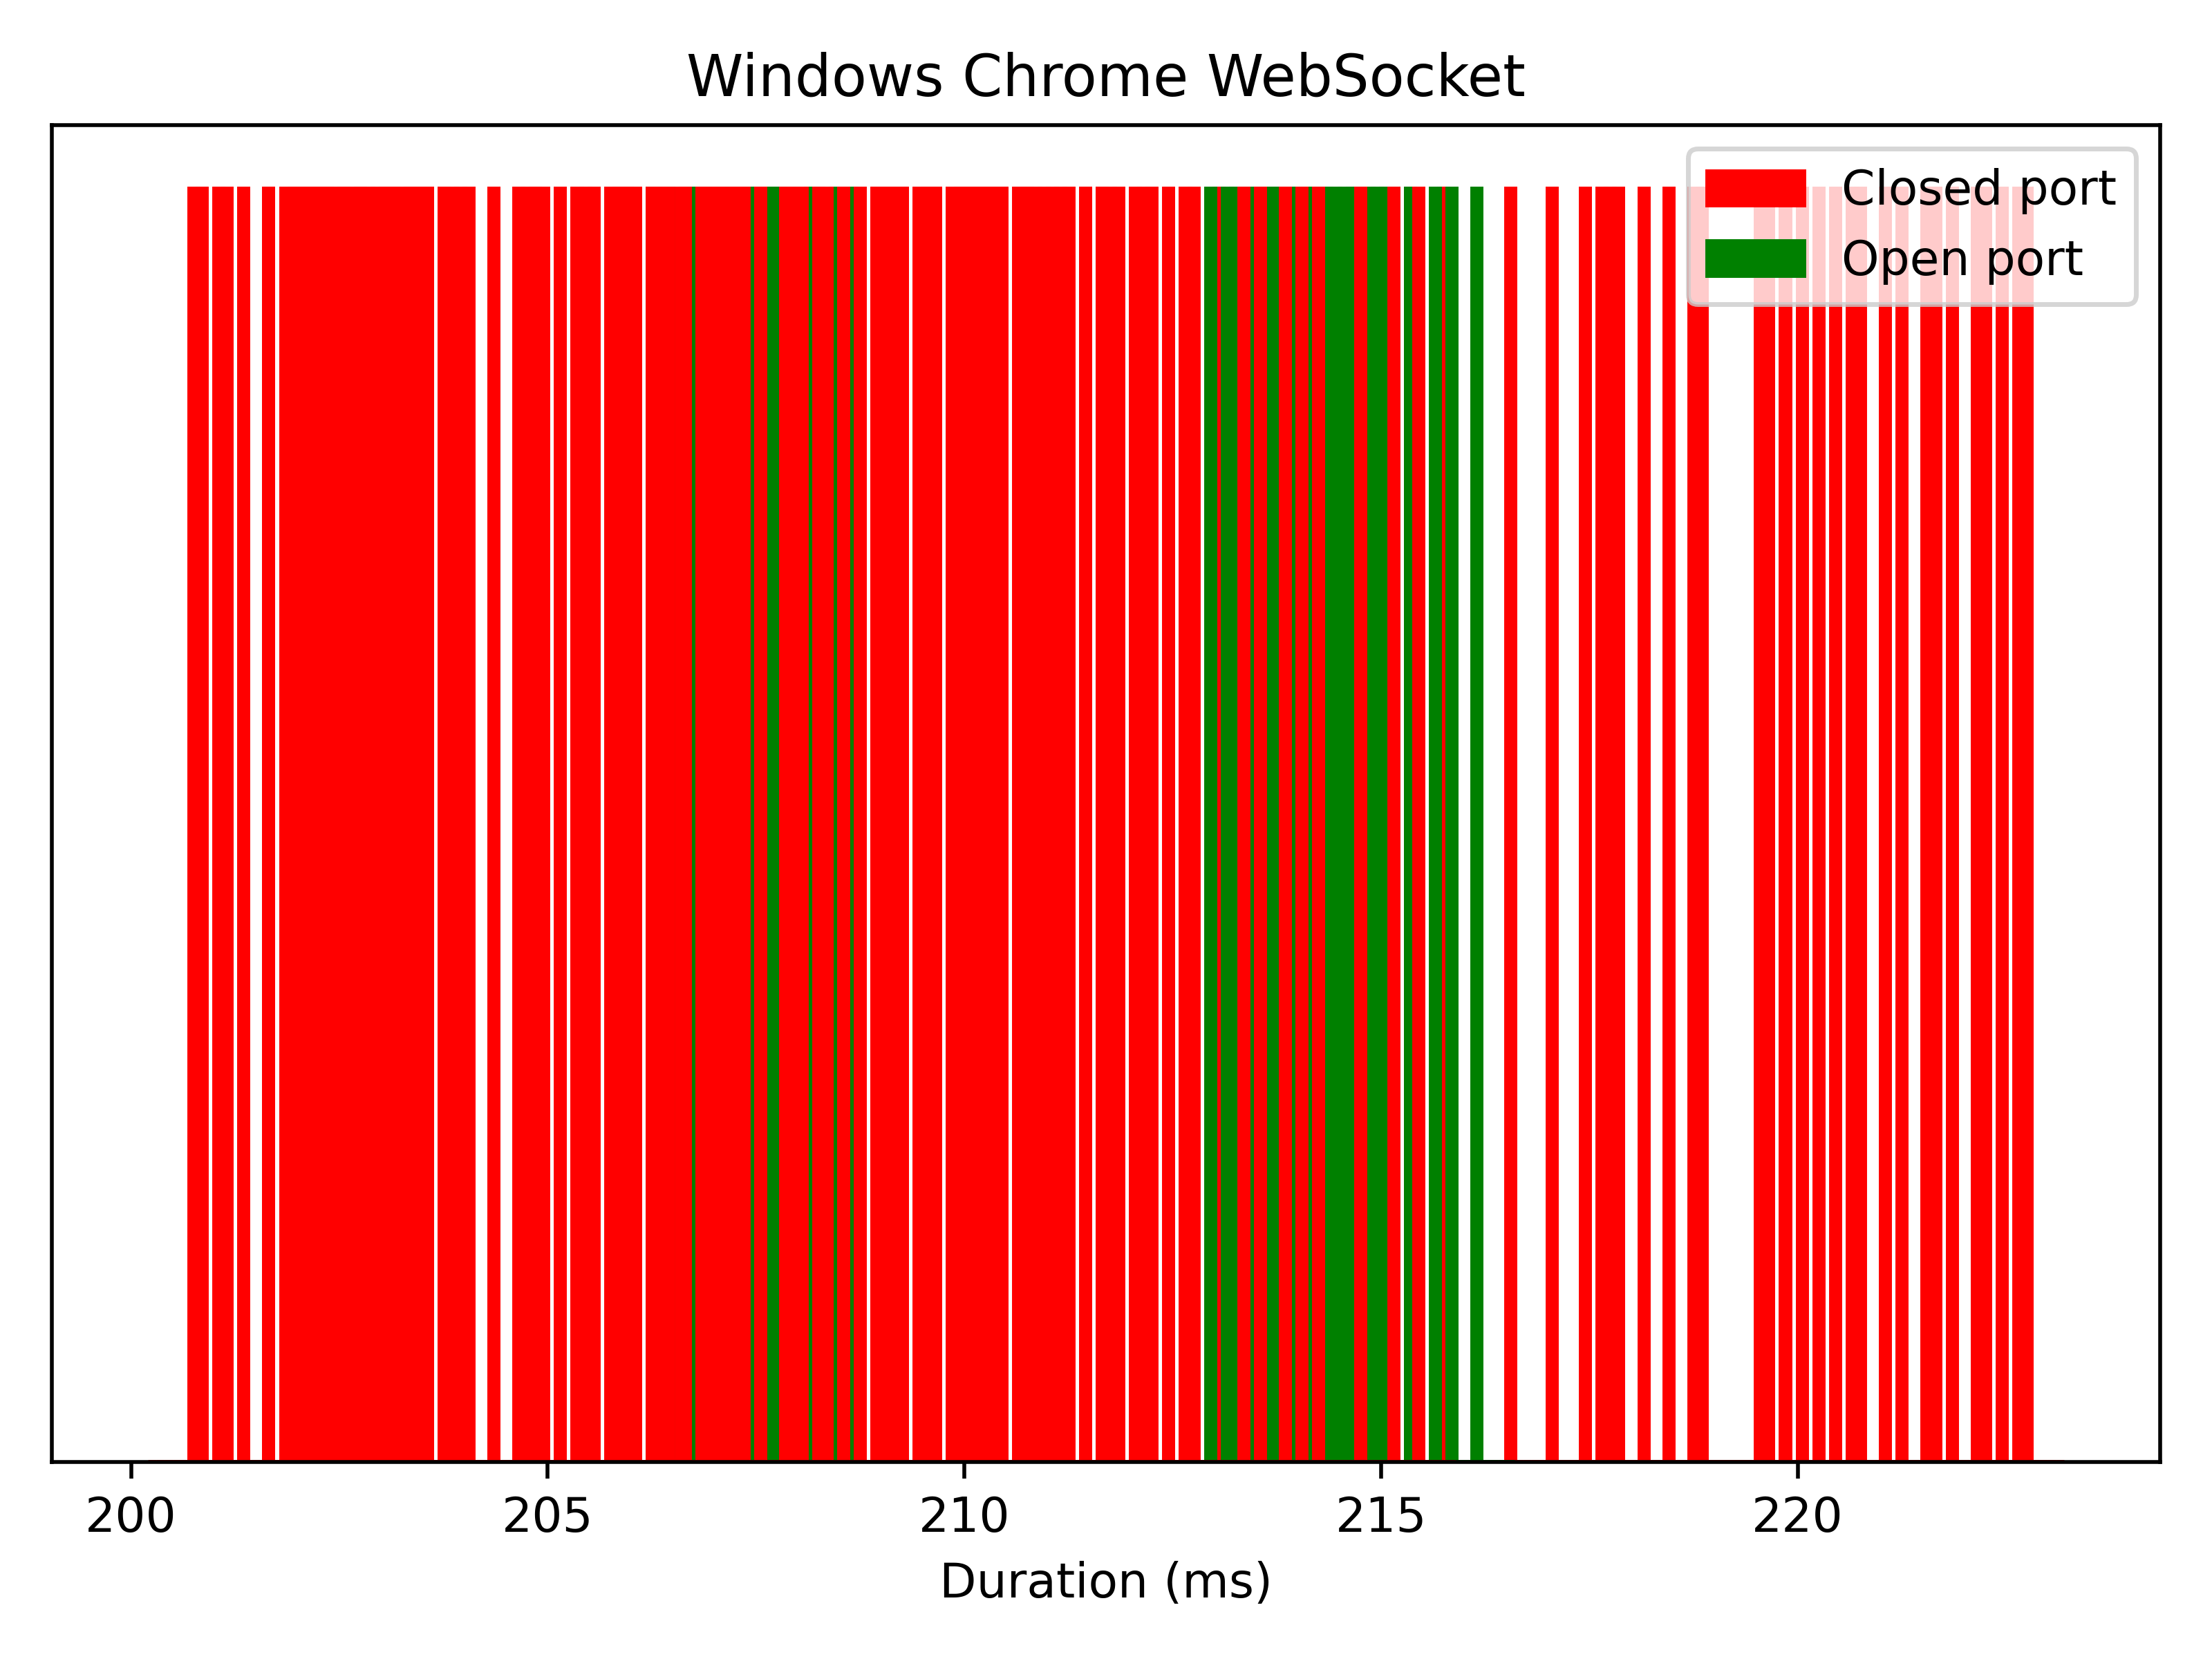
\includegraphics[width=8cm, height=4cm, keepaspectratio]{port_scanning_techniques/img/windows_chrome_efficacy_websocket.png}
    \caption{Windows/Chrome WebSocket API scan duration open vs closed ports}
    \label{fig:appendix-win-chrome-websocket}
\end{minipage}
\hspace{0.5cm} % Adjust the horizontal space between the two figures
\begin{minipage}{.45\textwidth}
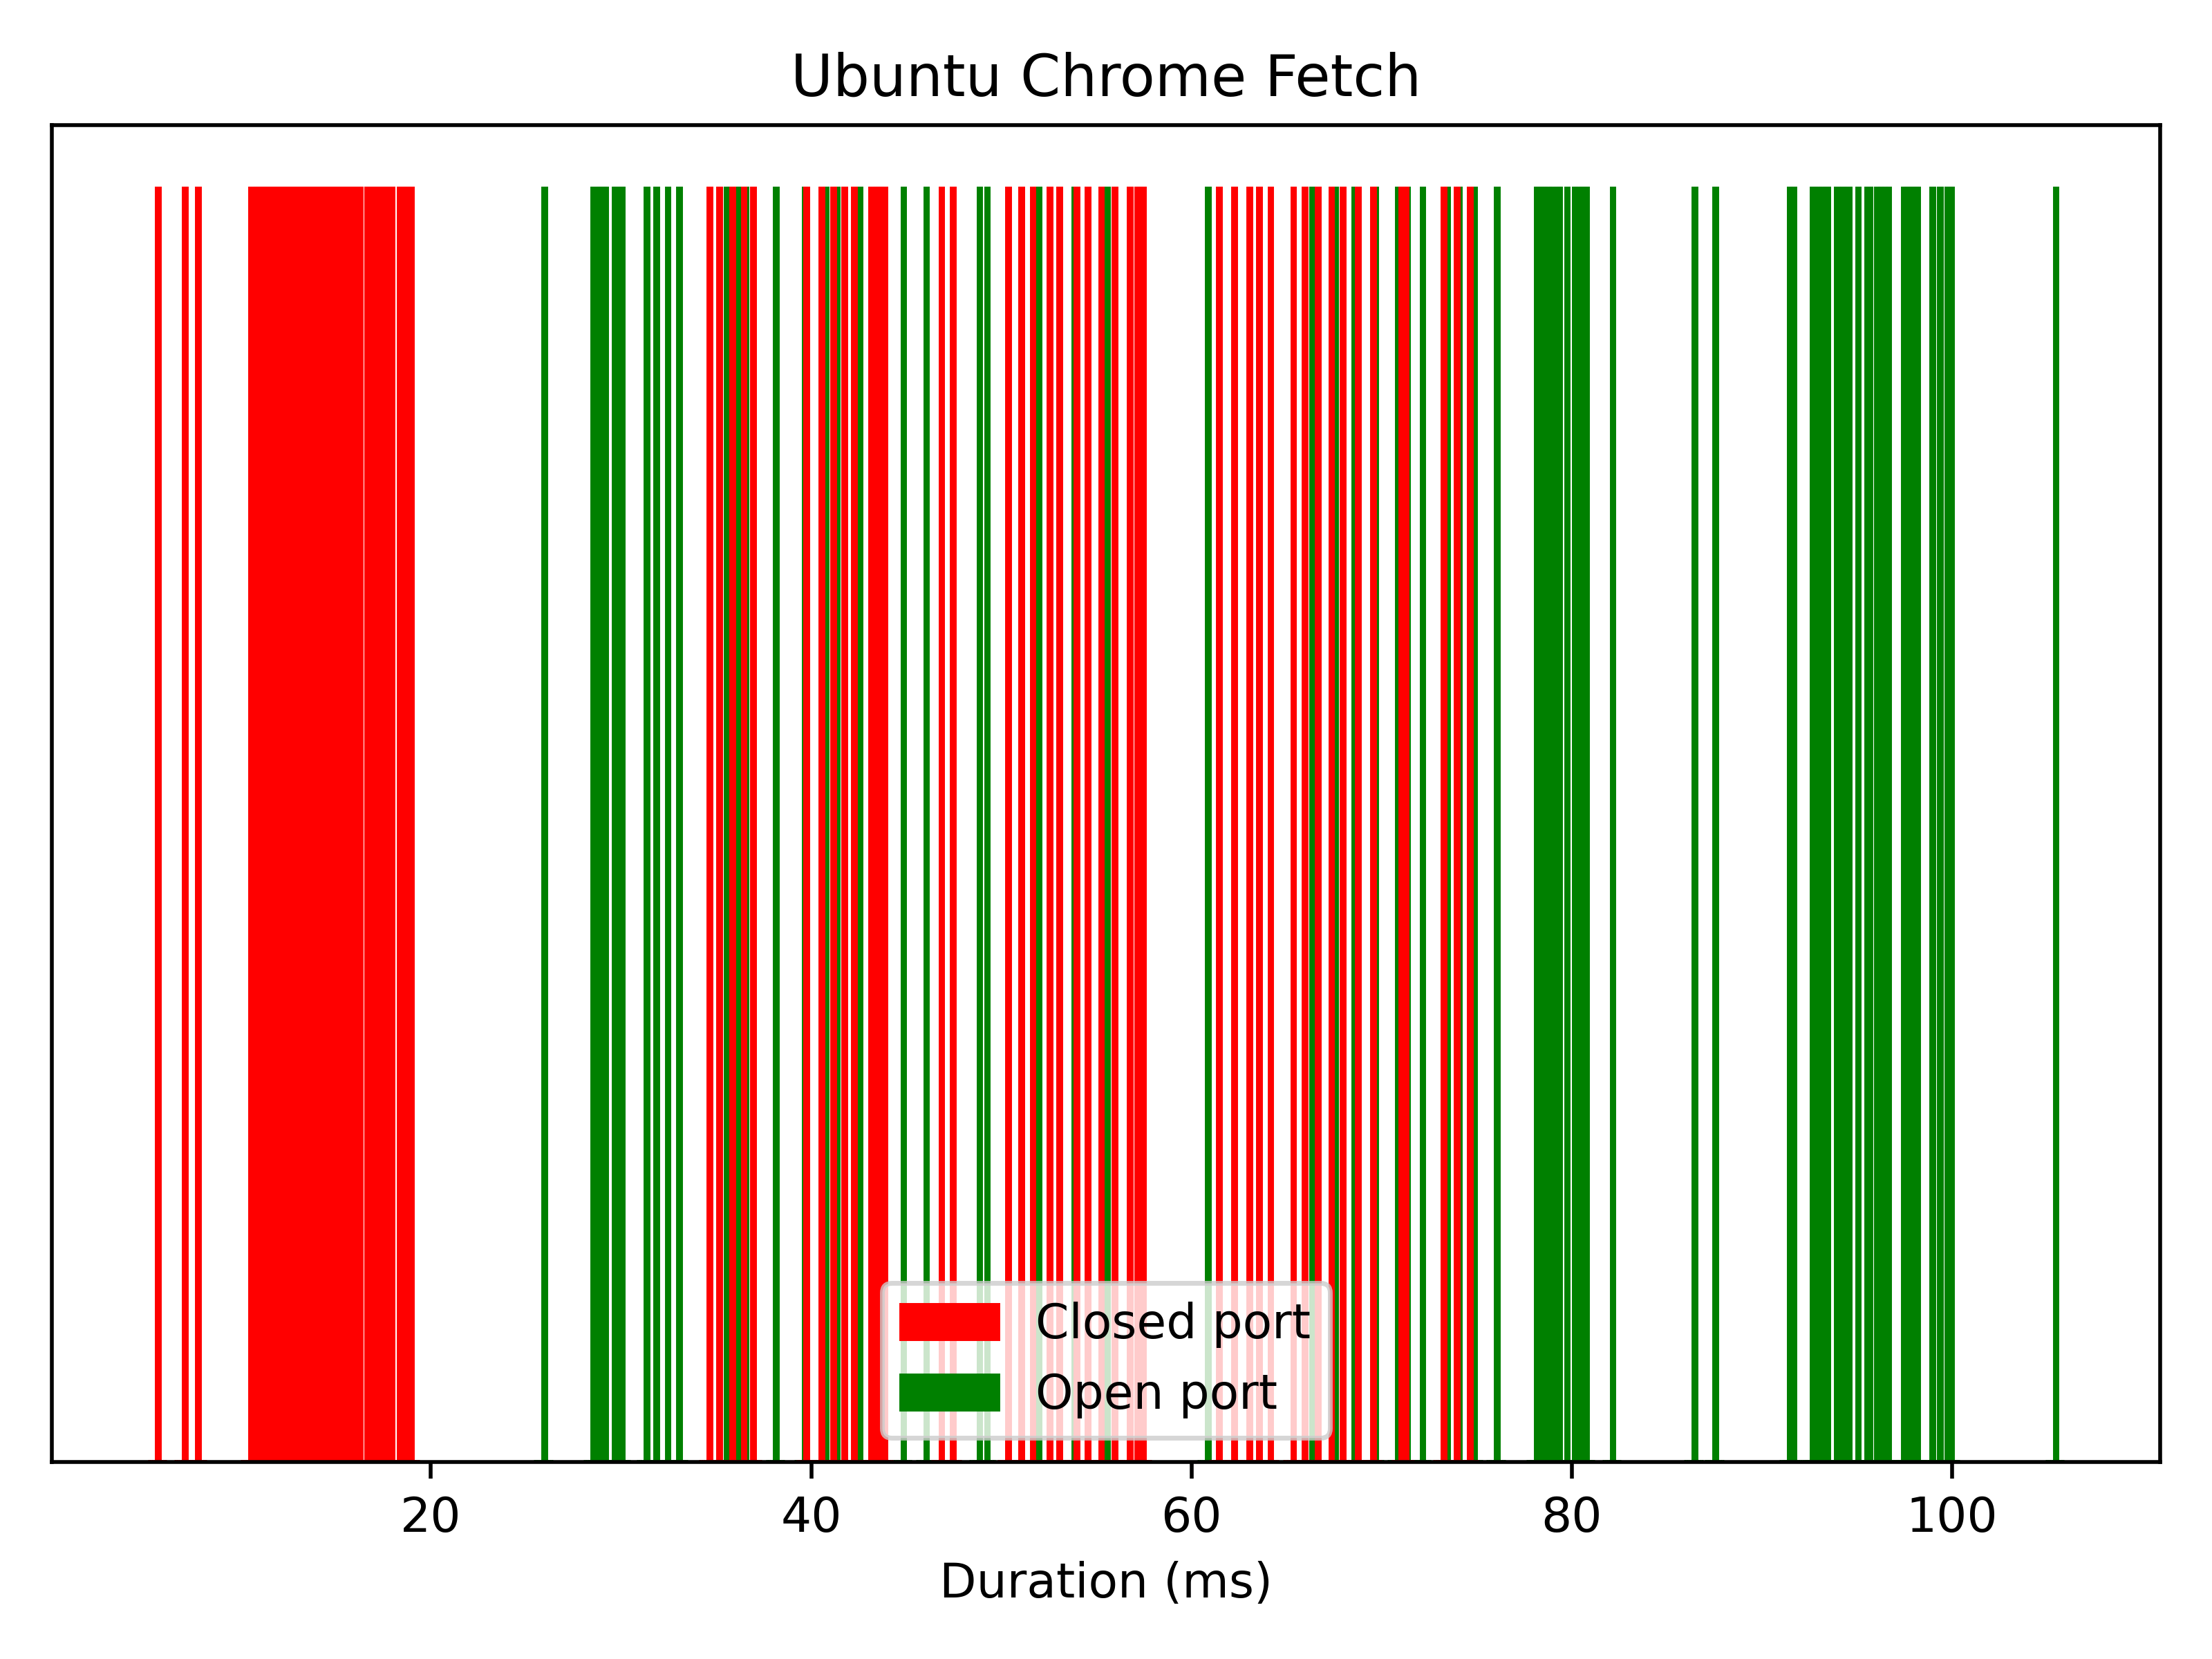
\includegraphics[width=8cm, height=4cm, keepaspectratio]{port_scanning_techniques/img/ubuntu_chrome_efficacy_fetch.png}
    \caption{Ubuntu/Chrome Fetch API scan duration open vs closed ports}
    \label{fig:ubuntu-chrome-fetch}
\end{minipage}
\end{figure}

\begin{figure}[ht]
\centering
\begin{minipage}{.45\textwidth}
  \centering
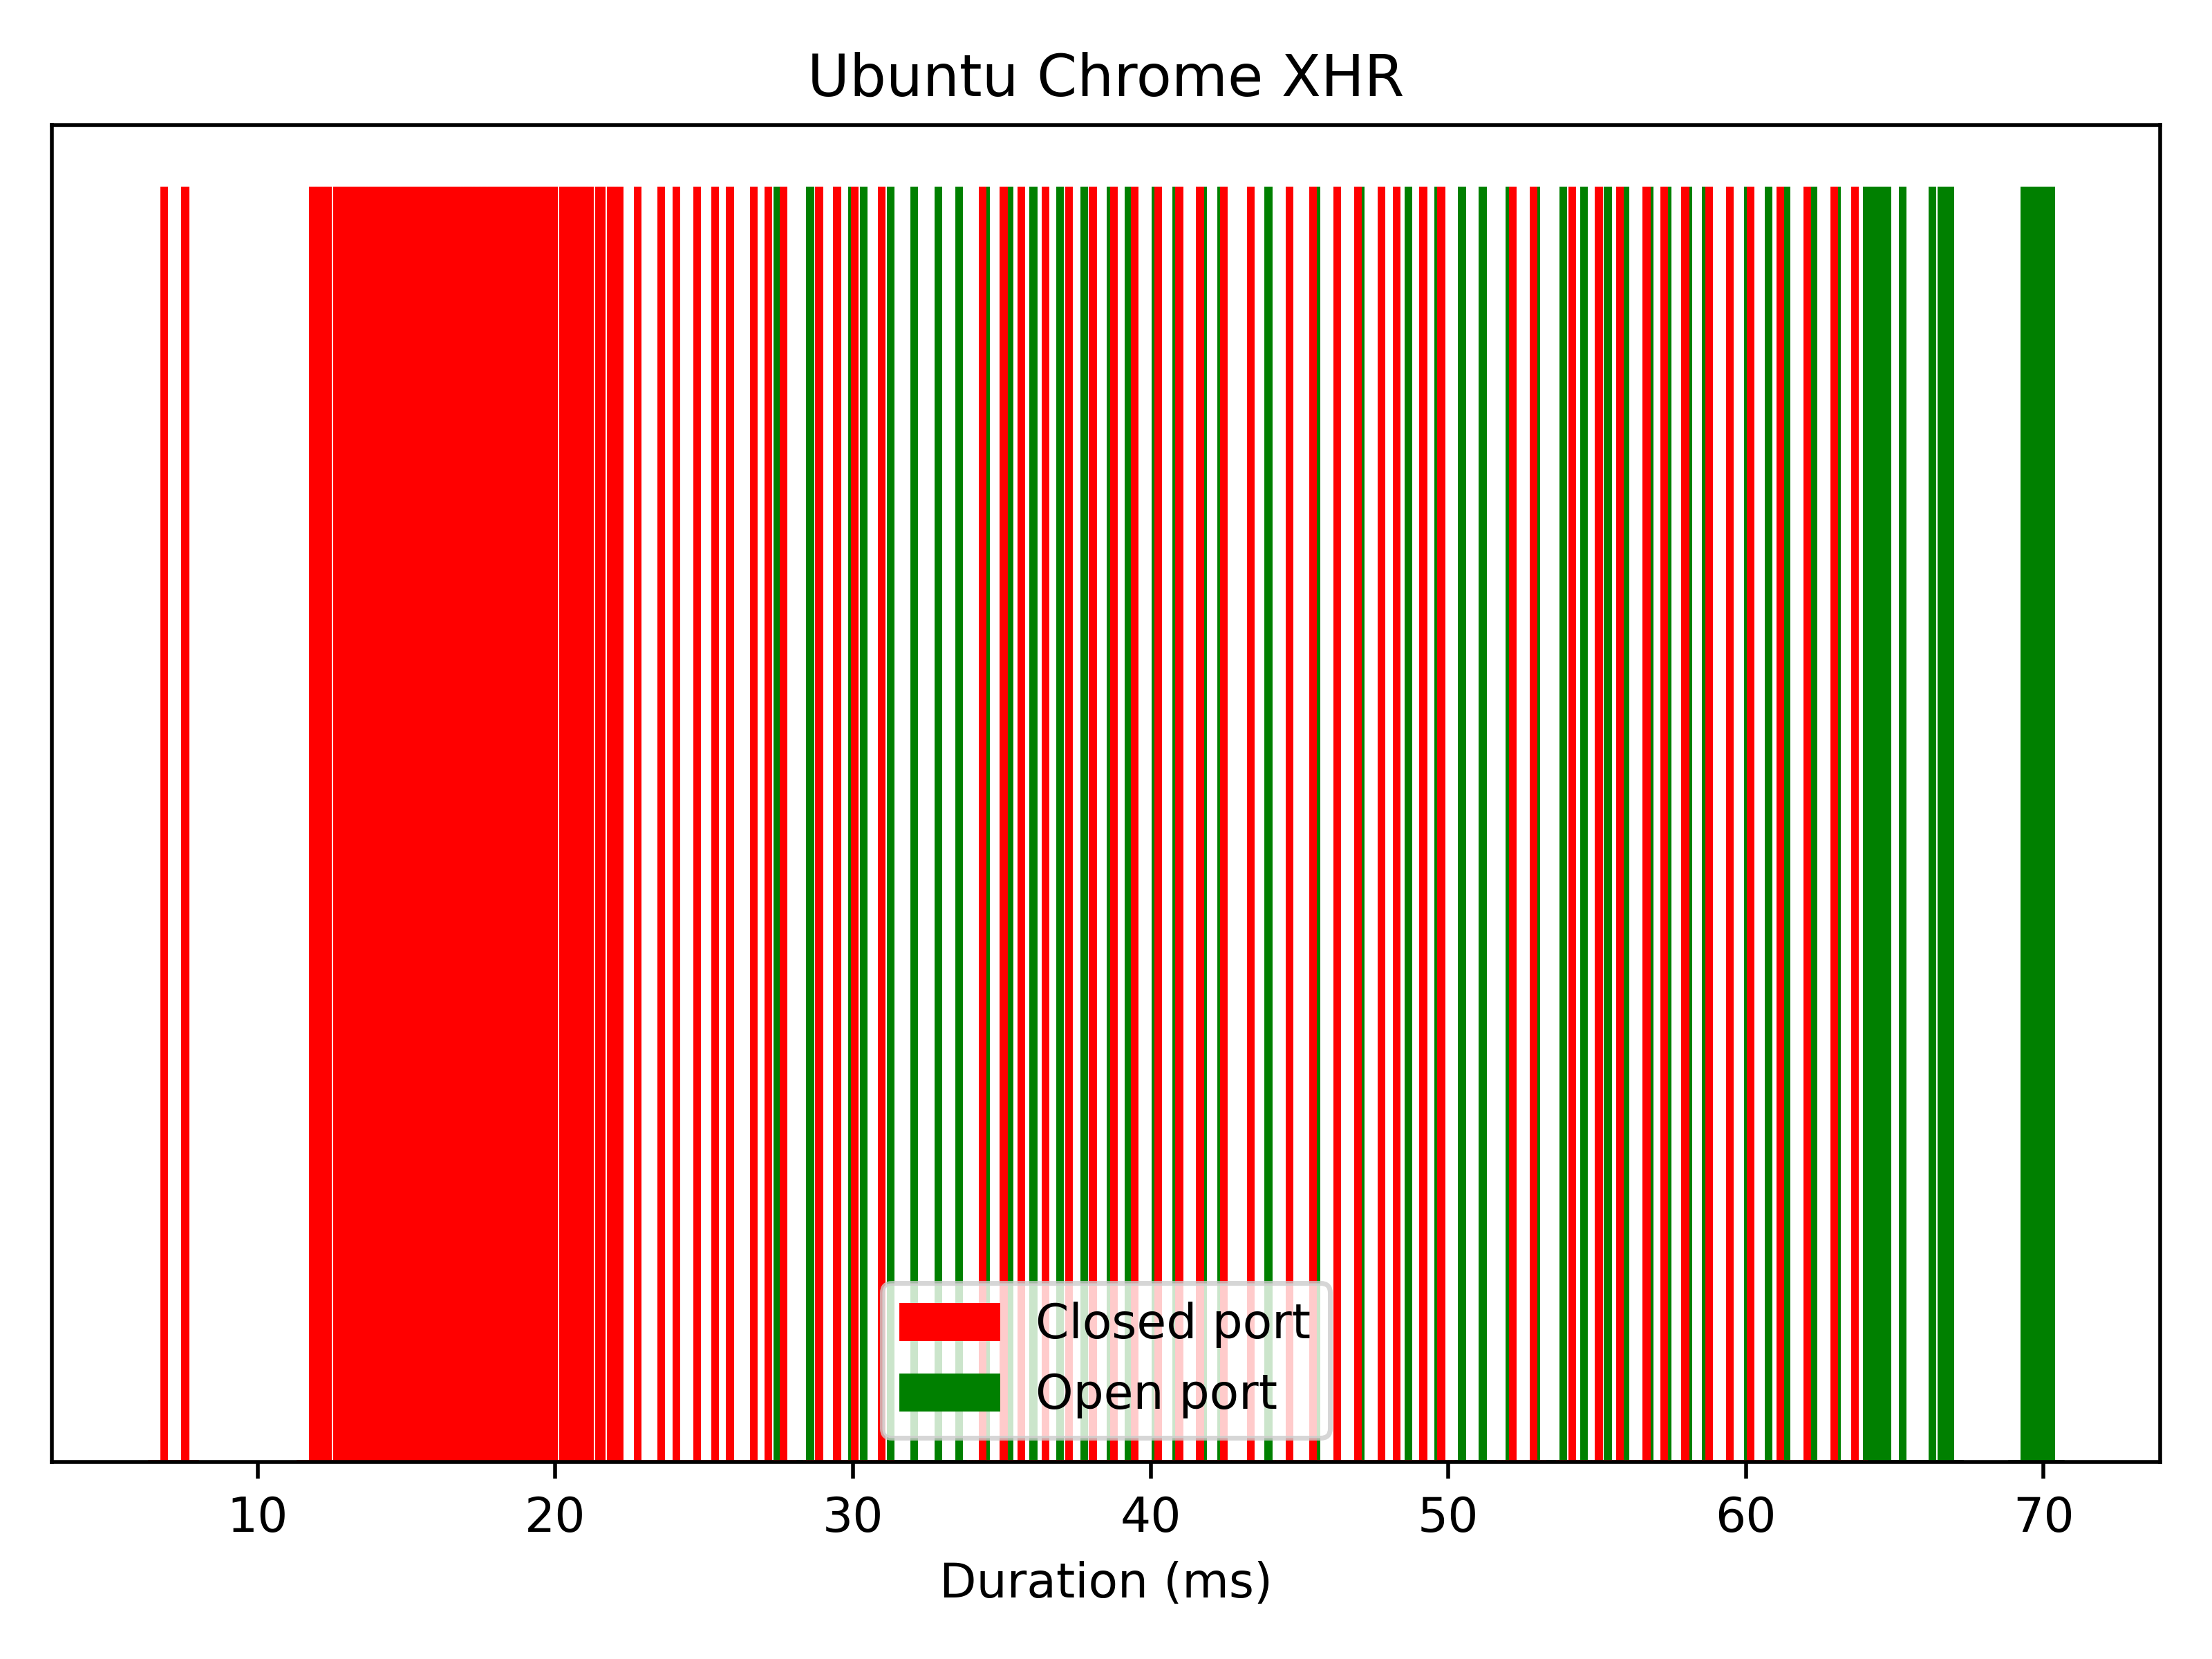
\includegraphics[width=8cm, height=4cm, keepaspectratio]{port_scanning_techniques/img/ubuntu_chrome_efficacy_xhr.png}
    \caption{Ubuntu/Chrome XHR API scan duration open vs closed ports}
    \label{fig:ubuntu-chrome-xhr}
\end{minipage}
\hspace{0.5cm} % Adjust the horizontal space between the two figures
\begin{minipage}{.45\textwidth}
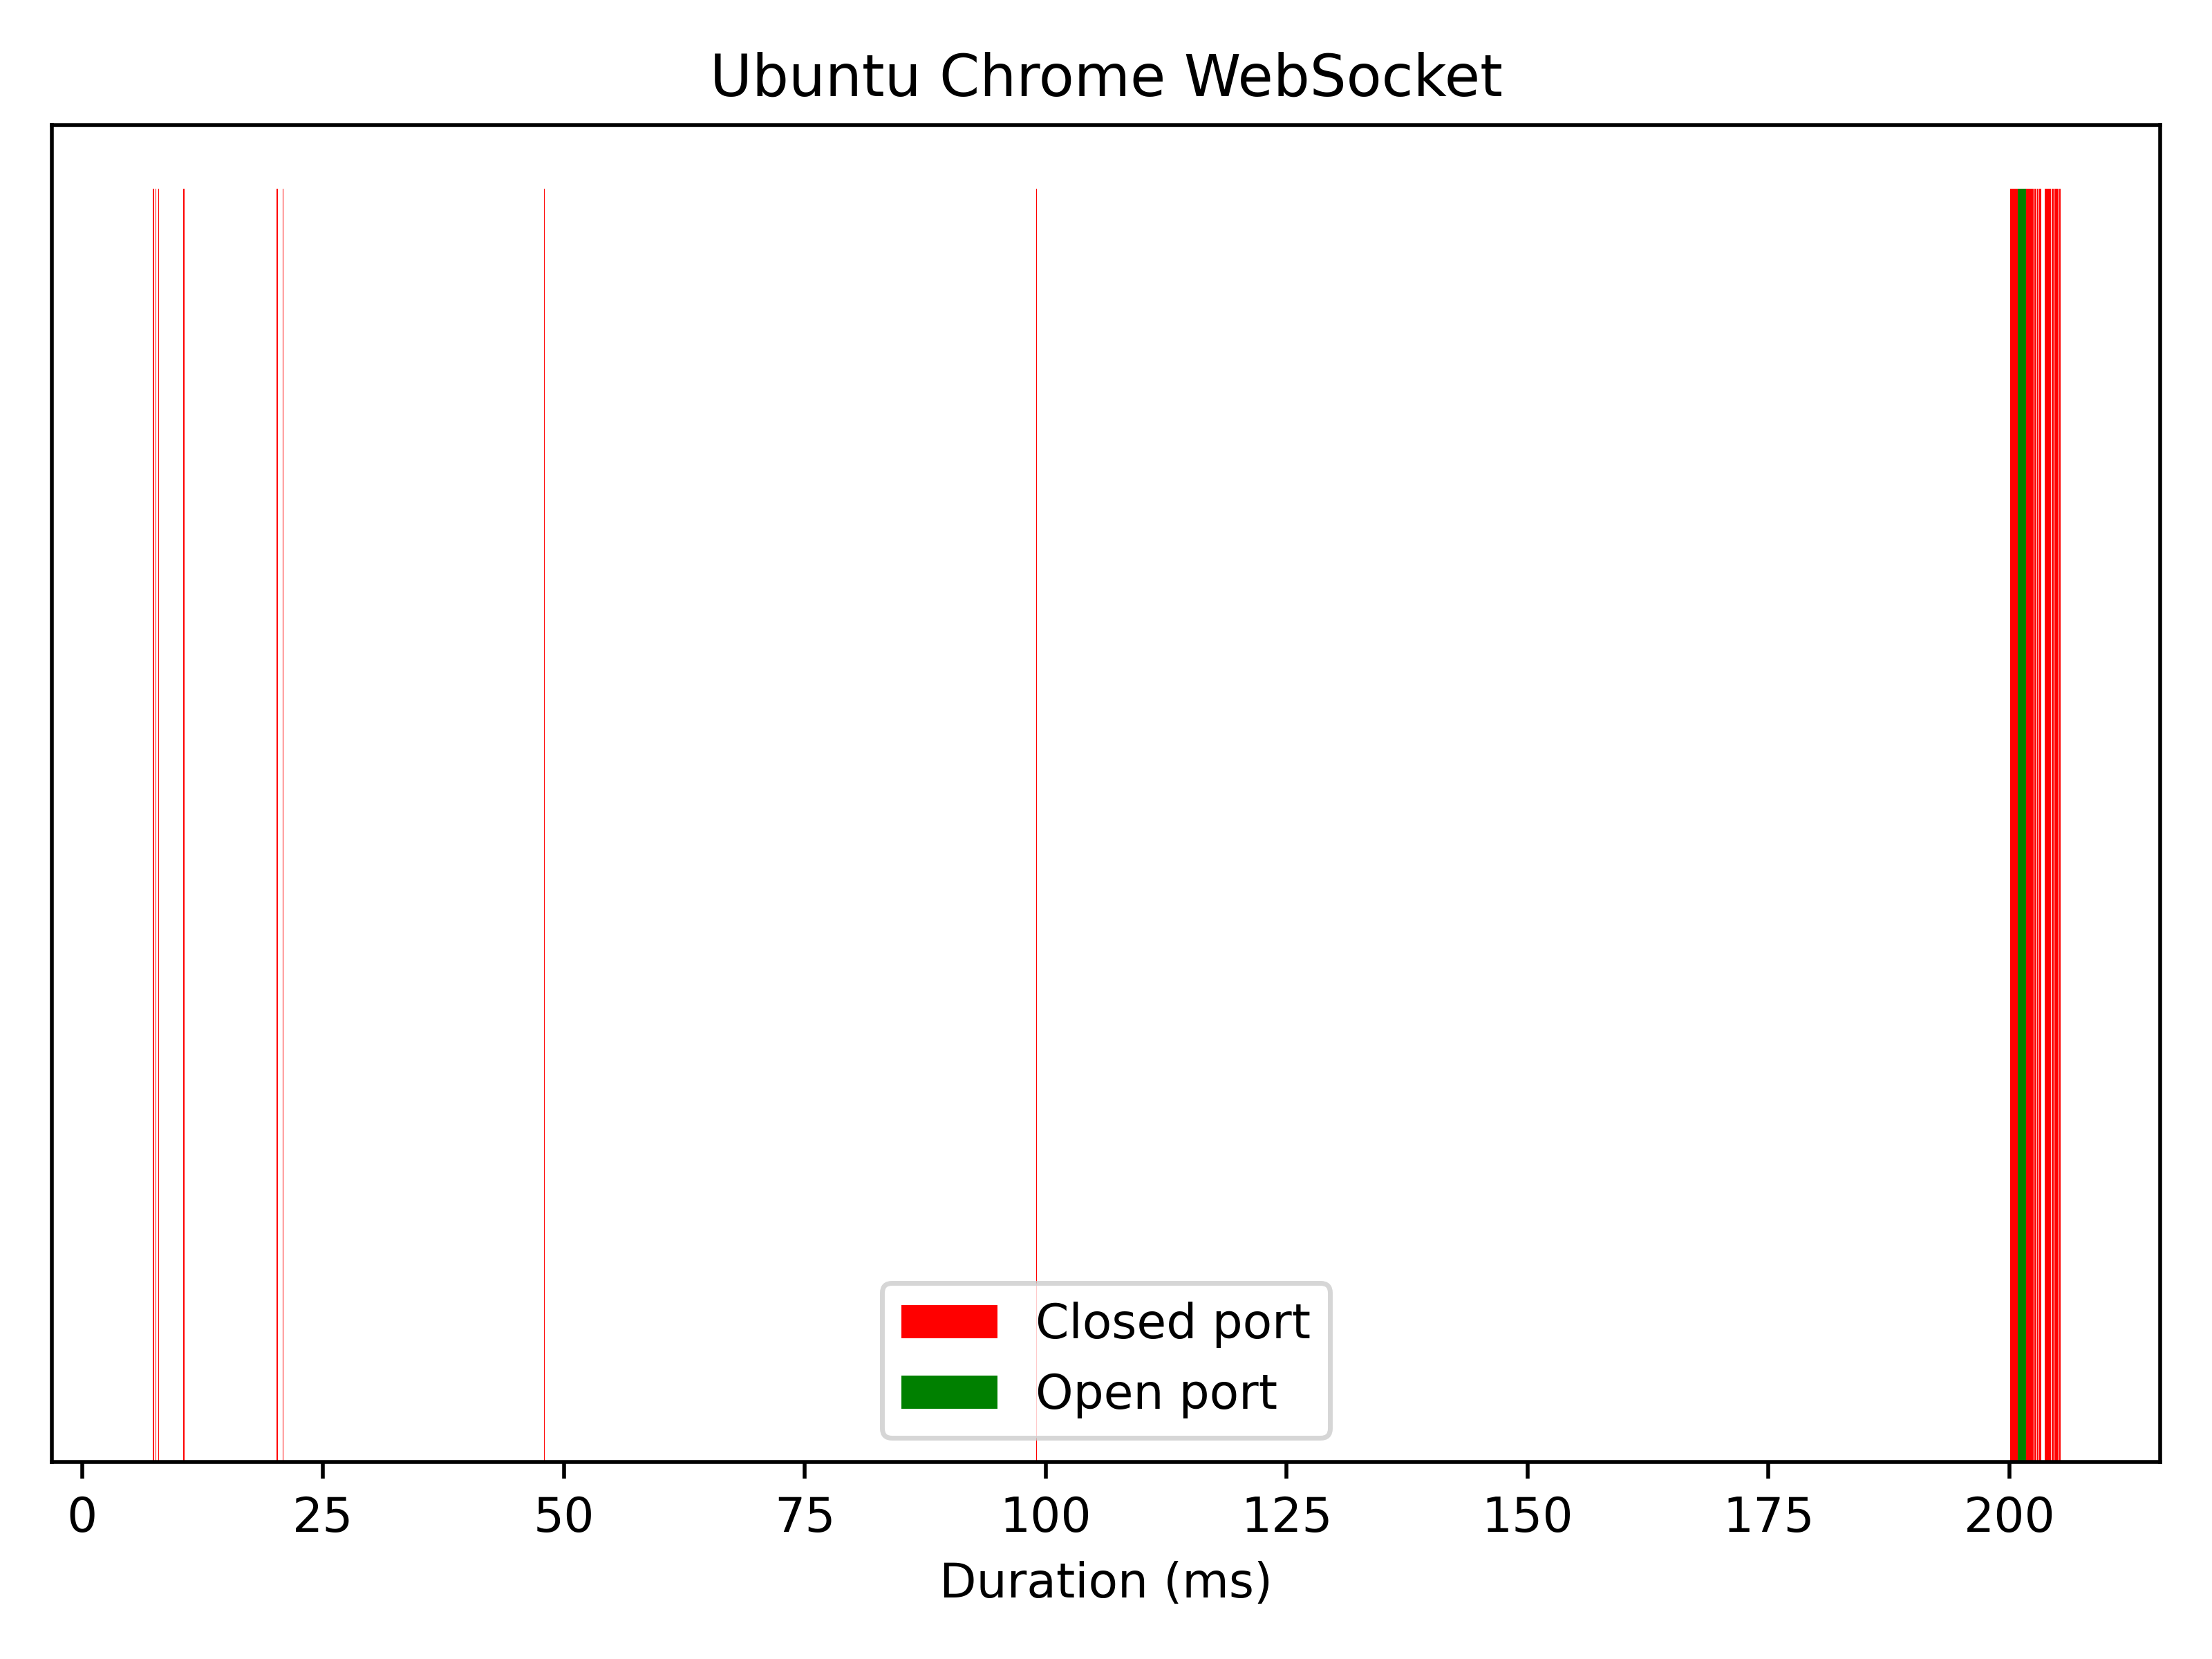
\includegraphics[width=8cm, height=4cm, keepaspectratio]{port_scanning_techniques/img/ubuntu_chrome_efficacy_websocket.png}
    \caption{Ubuntu/Chrome WebSocket API scan duration open vs closed ports}
    \label{fig:ubuntu-chrome-websocket}
\end{minipage}
\end{figure}

\begin{figure}[ht]
\centering
\begin{minipage}{.45\textwidth}
  \centering
\includegraphics[width=8cm, height=4cm, keepaspectratio]{port_scanning_techniques/img/windows_Firefox_efficacy_fetch.png}
    \caption{Windows/Firefox Fetch API scan duration open vs closed ports}
    \label{fig:win-firefox-fetch}
\end{minipage}
\hspace{0.5cm} % Adjust the horizontal space between the two figures
\begin{minipage}{.45\textwidth}
\includegraphics[width=8cm, height=4cm, keepaspectratio]{port_scanning_techniques/img/windows_Firefox_efficacy_xhr.png}
    \caption{Windows/Firefox XHR API scan duration open vs closed ports}
    \label{fig:appendix-win-firefox-xhr}
\end{minipage}
\end{figure}

\begin{figure}[ht]
\centering
\begin{minipage}{.45\textwidth}
  \centering
\includegraphics[width=8cm, height=4cm, keepaspectratio]{port_scanning_techniques/img/windows_Firefox_efficacy_websocket.png}
    \caption{Windows/Firefox WebSocket API scan duration open vs closed ports}
    \label{fig:appendix-win-firefox-websocket}
\end{minipage}
\hspace{0.5cm} % Adjust the horizontal space between the two figures
\begin{minipage}{.45\textwidth}
\includegraphics[width=8cm, height=4cm, keepaspectratio]{port_scanning_techniques/img/ubuntu_Firefox_efficacy_fetch.png}
    \caption{Ubuntu/Firefox Fetch API scan duration open vs closed ports}
    \label{fig:ubuntu-firefox-fetch}
\end{minipage}
\end{figure}

\begin{figure}[ht]
\centering
\begin{minipage}{.45\textwidth}
  \centering
\includegraphics[width=8cm, height=4cm, keepaspectratio]{port_scanning_techniques/img/ubuntu_Firefox_efficacy_xhr.png}
    \caption{Ubuntu/Firefox XHR API scan duration open vs closed ports}
    \label{fig:ubuntu-firefox-xhr}
\end{minipage}
\hspace{0.5cm} % Adjust the horizontal space between the two figures
\begin{minipage}{.45\textwidth}
\includegraphics[width=8cm, height=4cm, keepaspectratio]{port_scanning_techniques/img/ubuntu_Firefox_efficacy_websocket.png}
    \caption{Ubuntu/Firefox WebSocket API scan duration open vs closed ports}
    \label{fig:ubuntu-firefox-websocket}
\end{minipage}
\end{figure}
\clearpage

\section{Scanning techniques efficiency comparison}
\label{appendix:efficiency-comparison}

\begin{figure}[ht]
\begin{adjustwidth}{-3cm}{-1cm}
\centering
\begin{minipage}{.45\textwidth}
  \centering
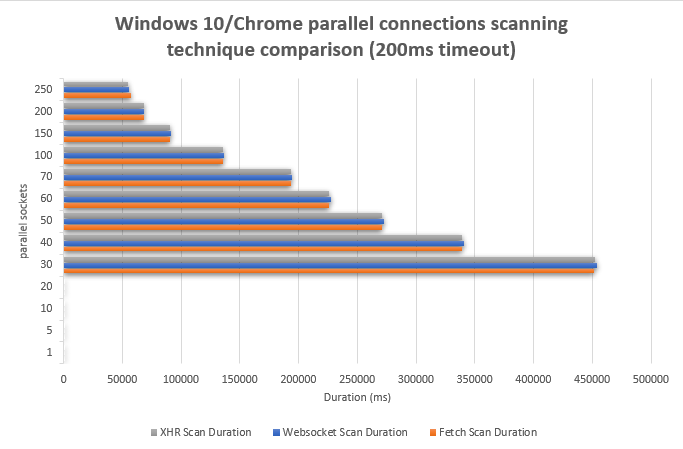
\includegraphics[width=10cm, height=7cm, keepaspectratio]{port_scanning_techniques/img/windows_chrome_scan_technique_comparison.png}
    \caption{Windows/Chrome Parallel sockets efficiency comparison}
    \label{fig:appendix-windows_chrome_n_sockets}
\end{minipage}
\hspace{3cm} % Adjust the horizontal space between the two figures
\begin{minipage}{.45\textwidth}
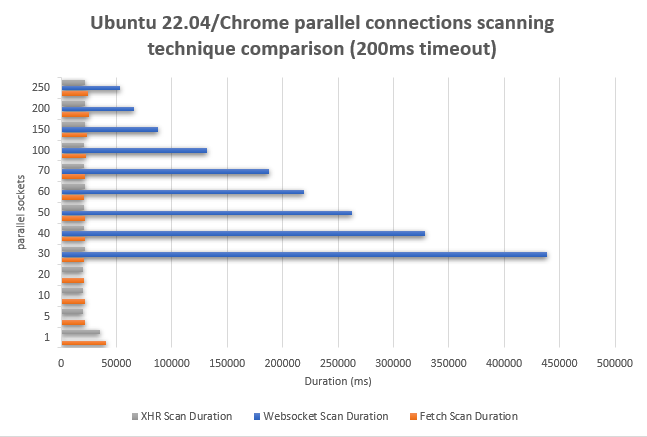
\includegraphics[width=10cm, height=7cm, keepaspectratio]{port_scanning_techniques/img/ubuntu_chrome_scan_technique_comparison.png}
    \caption{Ubuntu/Chrome Parallel sockets efficiency comparison}
    \label{fig:appendix-ubuntu_chrome_n_sockets}
\end{minipage}
\end{adjustwidth}
\end{figure}

\begin{figure}[ht]
\begin{adjustwidth}{-3cm}{-1cm}
\centering
\begin{minipage}{.45\textwidth}
  \centering
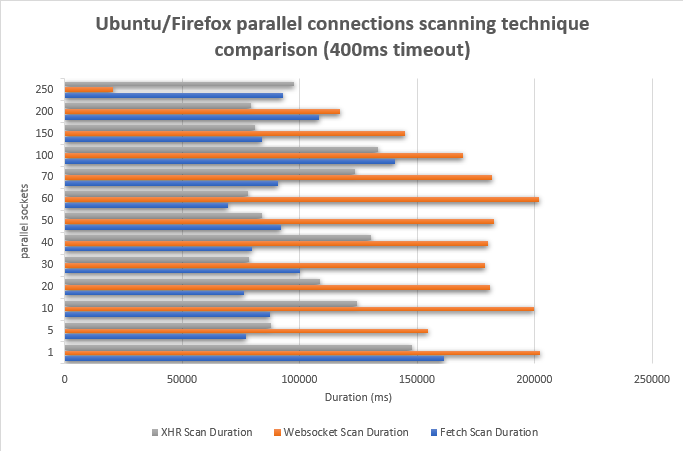
\includegraphics[width=10cm, height=7cm, keepaspectratio]{port_scanning_techniques/img/ubuntu_firefox_scan_technique_comparison.png}
    \caption{Ubuntu/Firefox Parallel sockets efficiency comparison}
    \label{fig:ubuntu_firefox_n_sockets}
\end{minipage}
\hspace{3cm} % Adjust the horizontal space between the two figures
\begin{minipage}{.45\textwidth}
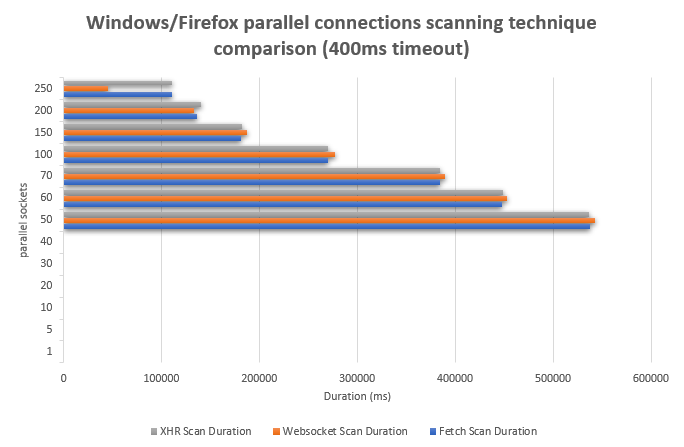
\includegraphics[width=10cm, height=7cm, keepaspectratio]{port_scanning_techniques/img/windows_firefox_scan_technique_comparison.png}
    \caption{Windows/Firefox Parallel sockets efficiency comparison}
    \label{fig:windows_firefox_n_sockets}
\end{minipage}
\end{adjustwidth}
\end{figure}
%  \input{Appendices/appendix-b}
%  \input{Appendices/appendix-c}


\end{document}
